%% LyX 2.0.3 created this file.  For more info, see http://www.lyx.org/.
%% Do not edit unless you really know what you are doing.
\documentclass[twoside,english]{paper}
\usepackage{lmodern}
\renewcommand{\ttdefault}{lmodern}
\usepackage[T1]{fontenc}
\usepackage[latin9]{inputenc}
\usepackage[a4paper]{geometry}
\geometry{verbose,tmargin=3cm,bmargin=2.5cm,lmargin=2cm,rmargin=2cm}
\usepackage{color}
\usepackage{babel}
\usepackage{float}
\usepackage{bm}
\usepackage{amsthm}
\usepackage{amsmath}
\usepackage{amssymb}
\usepackage{graphicx}
\usepackage{esint}
\usepackage[unicode=true,pdfusetitle,
 bookmarks=true,bookmarksnumbered=false,bookmarksopen=false,
 breaklinks=false,pdfborder={0 0 0},backref=false,colorlinks=false]
 {hyperref}
\usepackage{breakurl}

\makeatletter

%%%%%%%%%%%%%%%%%%%%%%%%%%%%%% LyX specific LaTeX commands.
%% Because html converters don't know tabularnewline
\providecommand{\tabularnewline}{\\}

%%%%%%%%%%%%%%%%%%%%%%%%%%%%%% Textclass specific LaTeX commands.
\numberwithin{equation}{section}
\numberwithin{figure}{section}

%%%%%%%%%%%%%%%%%%%%%%%%%%%%%% User specified LaTeX commands.
\usepackage{babel}

\@ifundefined{showcaptionsetup}{}{%
 \PassOptionsToPackage{caption=false}{subfig}}
\usepackage{subfig}
\makeatother

\begin{document}

\title{QED corrections to parton distribution functions}


\author{Valerio Bertone$^{a}$, Stefano Carrazza$^{b}$}


\institution{$^{a}$Physikalisches Institut, Albert-Ludwigs-Universit\"{a}t Freiburg\\
$^{b}$Dipartimento di Fisica, Universit� di Milano and INFN}
\maketitle
\begin{abstract}
In this document we present the method to be used in order to apply
QED corrections in QCD evolution and obtain the PDF of photons. 
\end{abstract}
\tableofcontents{}

\newpage{}


\part{Theory}


\section{Motivation}

The introduction of QED effects, when computing the parton distribution
functions, is justified by the fact that 
\begin{equation}
\frac{\alpha_{s}^{2}(M_{Z}^{2})}{\alpha(M_{Z}^{2})}\sim\frac{0.1184^{2}}{1/127}\sim1.78
\end{equation}
in other words, the QED coupling $\alpha$ can affects processes in
which QCD predictions are computed at NLO and higher orders. On the
other hand the introduction of QED corrections implies the extraction
of the photon's PDF. In the next we will limit ourselves to QED corrections
at LO.


\section{Some QED properties}


\subsection{The QED evolution equation}

From Gribov and Lipatov, the evolution equations for QED take the
form (\cite{Peskin} pag. 586) 
\begin{equation}
Q^{2}\frac{\partial}{\partial Q^{2}}\left(\begin{array}{c}
\gamma\\
e\\
\bar{e}
\end{array}\right)(x,Q^{2})=\frac{\alpha(Q^{2})}{2\pi}\int_{x}^{1}\frac{d\xi}{\xi}\left(\begin{array}{ccc}
P_{\gamma\gamma}(\xi) & P_{\gamma e}(\xi) & P_{\gamma e}(\xi)\\
P_{e\gamma}(\xi) & P_{ee}(\xi) & 0\\
P_{e\gamma}(\xi) & 0 & P_{ee}(\xi)
\end{array}\right)\left(\begin{array}{c}
\gamma\\
e\\
\bar{e}
\end{array}\right)\left(\frac{x}{\xi},Q^{2}\right)
\end{equation}
where $P_{ij}(\xi)$ are the splitting functions defined at leading
order as (\cite{Peskin} pag. 587) 
\begin{equation}
P_{\gamma\gamma}^{(0)}(\xi)=-\frac{2}{3}\delta(1-\xi)
\end{equation}
\begin{equation}
P_{\gamma e}^{(0)}(\xi)=\frac{1+(1-\xi)^{2}}{\xi}
\end{equation}
\begin{equation}
P_{e\gamma}^{(0)}(\xi)=\xi^{2}+\left(1-\xi\right)^{2}
\end{equation}
\begin{equation}
P_{ee}^{(0)}(\xi)=\frac{1+\xi^{2}}{\left(1-\xi\right)_{+}}+\frac{3}{2}\delta(1-\xi)
\end{equation}


The momentum sum rules must satisfy the following relation 
\begin{equation}
\int_{0}^{1}dx\left[e\left(x,Q^{2}\right)-\bar{e}\left(x,Q^{2}\right)\right]=\int_{0}^{1}dx\, x\left[e\left(x,Q^{2}\right)+\bar{e}\left(x,Q^{2}\right)+\gamma\left(x,Q^{2}\right)\right]=1
\end{equation}



\subsection{The QED running coupling $\alpha(Q^{2})$}

The 1-loop $\beta(\alpha)$ function in QED is 
\begin{equation}
\beta(\alpha)=Q^{2}\frac{\partial\alpha}{\partial Q^{2}}=\beta_{0}\alpha^{2}=\frac{2\alpha^{2}}{3\pi}\qquad\text{(LO)}\label{eq:betafunction}
\end{equation}
written in terms of the QED coupling constant $\alpha$, with $\beta_{0}=2/3\pi$.
Lets solve Eq. (\ref{eq:betafunction}) in order to obtain $\alpha(Q^{2})$
in function of $\alpha(Q_{0}^{2})$ 
\begin{equation}
\int_{\alpha(Q_{0}^{2})}^{\alpha(Q^{2})}\frac{d\alpha'}{\beta_{0}\alpha'^{2}}=\int_{Q_{0}^{2}}^{Q^{2}}\frac{dQ'^{2}}{Q'^{2}}
\end{equation}
and we obtain 
\begin{equation}
\alpha(Q^{2})=\alpha(Q_{0}^{2})\left(1-\beta_{0}\alpha(Q_{0}^{2})\ln\frac{Q^{2}}{Q_{0}^{2}}\right)^{-1}\qquad\text{(LO)}
\end{equation}
where $Q_{0}^{2}$ is fixed a priori by some reference experimental
value. When we consider QED correction in QCD we must redefine the
$\beta$ function in function of the quark charges $e_{q_{i}}$ and
the color multiplicity $N_{c}^{i}$ 
\begin{equation}
\beta_{0}=\frac{2}{3\pi}\sum_{f=e,\mu,\tau,u,d,s,c,b,t}N_{c}^{f}e_{q_{f}}^{2}
\end{equation}



\section{QED corrections in the QCD evolution}


\subsection{Breaking isospin conservation}

The most important difference between pure QCD and QED processes is
that electrical charges appears, breaking the isospin conservation.
Partons are dependent of nucleons, e.g. proton partons are different
from neutron partons.

The important remark is that when computing the evolution kernels
for these PDFs, we observe that in the DGLAP equation splitting functions
are independent from the nature of these partons, so we just need
to compute kernels once, and then decide or not to apply the symmetry
breaking between PDFs when fitting the data provided by different
experiments.


\subsection{Decoupling QCD and QED evolution}

Supposing the factorization scale of QCD and QED may have different
values or be equal one can write the solution of the DGLAP equation
as 
\begin{equation}
f_{i}(N,Q_{\text{QED}}^{2},Q_{0,\text{QCD}}^{2})=\Gamma_{ij}^{\text{QED}}(N,Q_{\text{QED}}^{2},Q_{0,\text{QED}}^{2})\cdot f_{j}(N,Q_{0,\text{QED}}^{2},Q_{0,\text{QCD}}^{2})
\end{equation}
so 
\begin{equation}
f_{i}(N,Q_{\text{QED}}^{2},Q_{\text{QCD}}^{2})=\Gamma_{ik}^{\text{QCD}}(N,Q_{\text{QCD}}^{2},Q_{0,\text{QCD}}^{2})\cdot\Gamma_{kj}^{\text{QED}}(N,Q_{\text{QED}}^{2},Q_{0,\text{QED}}^{2})\cdot f_{j}(N,\, Q_{0,\text{QED}}^{2},\, Q_{0,\text{QCD}}^{2})
\end{equation}
if the factorization scale is the same for both 
\begin{equation}
f_{i}(N,Q^{2})=\Gamma_{ik}^{\text{QCD}}(N,Q^{2},Q_{0}^{2})\cdot\Gamma_{kj}^{\text{QED}}(N,Q^{2},Q_{0}^{2})\cdot f_{j}(N,Q_{0,}^{2})
\end{equation}
where, as we are working with matrices, using the Baker\textendash{}Campbell\textendash{}Hausdorff
formula one obtains 
\begin{equation}
\Gamma_{ik}^{\text{QCD}}(N,Q^{2},Q_{0}^{2})\cdot\Gamma_{kj}^{\text{QED}}(N,Q^{2},Q_{0}^{2})=\Gamma_{ik}^{\text{QED}}(N,Q^{2},Q_{0}^{2})\cdot\Gamma_{kj}^{\text{QCD}}(N,Q^{2},Q_{0}^{2})+\mathcal{O}(\alpha\alpha_{S})
\end{equation}


This is strategy is the fastest way to introduce QED corrections in
the current NNPDF code.


\subsection{General solution of DGLAP equations}

We can write the DGLAP equation in Mellin space as 
\begin{equation}
Q^{2}\frac{\partial}{\partial Q^{2}}\mathbf{\underline{f}}(N,Q^{2})=\frac{\alpha(Q^{2})}{2\pi}\mathbf{A}(N)\cdot\mathbf{\underline{f}}(N,Q^{2})\label{eq:dglap}
\end{equation}
by using the running coupling equation (\ref{eq:betafunction}) we
get 
\begin{equation}
Q^{2}\frac{\partial}{\partial Q^{2}}=\beta_{0}\alpha^{2}(Q^{2})\frac{\partial}{\partial\alpha(Q^{2})}
\end{equation}
so eq. (\ref{eq:dglap}) becomes 
\begin{equation}
\frac{\partial}{\partial\alpha(Q^{2})}\mathbf{\underline{f}}(N,Q^{2})=\frac{1}{2\pi\beta_{0}\alpha(Q^{2})}\mathbf{A}(N)\cdot\mathbf{\underline{f}}(N,Q^{2})
\end{equation}
where we redefined $\beta_{0}=\frac{2}{3\pi}\sum_{i}^{n_{f}}N_{c}^{i}e_{q_{i}}^{2}$.
The solution is given by 
\begin{equation}
\int_{\mathbf{\underline{f}}(N,Q_{0}^{2})}^{\mathbf{\underline{f}}(N,Q^{2})}\frac{d\mathbf{\underline{f}}}{\mathbf{\underline{f}}}=\frac{\mathbf{A}(N)}{2\pi\beta_{0}}\int_{\alpha(Q_{0}^{2})}^{\alpha(Q^{2})}\frac{d\alpha}{\alpha}
\end{equation}
so the solution is 
\begin{eqnarray}
\mathbf{\underline{f}}(N,Q^{2}) & = & \left(\frac{\alpha(Q^{2})}{\alpha(Q_{0}^{2})}\right)^{\mathbf{A}(N)/2\pi\beta_{0}}\mathbf{\underline{f}}(N,Q_{0}^{2})\\
 & = & \text{exp}\left[\frac{\mathbf{A}(N)}{2\pi\beta_{0}}\ln\frac{\alpha(Q^{2})}{\alpha(Q_{0}^{2})}\right]\cdot\mathbf{\underline{f}}(N,Q_{0}^{2})\\
 & = & \mathbf{\Gamma}(N,Q^{2},Q_{0}^{2})\cdot\mathbf{\underline{f}}(N,Q_{0}^{2})
\end{eqnarray}


The only difficulty is the calculation of the exponential if the matrix
$\mathbf{A}(N)$ has non zero diagonal terms. This can be achieved
by diagonalizing $\mathbf{A}(N)$ and solving in this diagonal form.


\subsection{QED evolution}

The QED evolution equation for partons is given by 
\begin{equation}
Q^{2}\frac{\partial}{\partial Q^{2}}\gamma(x,Q^{2})=\frac{\alpha(Q^{2})}{2\pi}\int_{x}^{1}\frac{d\xi}{\xi}\left\{ P_{\gamma\gamma}(\xi)e_{\Sigma}^{2}\gamma\left(\frac{x}{\xi},Q^{2}\right)+P_{\gamma q}(\xi)\underset{j}{\sum}e_{j}^{2}q_{j}\left(\frac{x}{\xi},Q^{2}\right)\right\} 
\end{equation}
\begin{equation}
Q^{2}\frac{\partial}{\partial Q^{2}}q_{i}(x,Q^{2})=\frac{\alpha(Q^{2})}{2\pi}\int_{x}^{1}\frac{d\xi}{\xi}\left\{ P_{q\gamma}(\xi)e_{i}^{2}\gamma\left(\frac{x}{\xi},Q^{2}\right)+P_{qq}(\xi)e_{i}^{2}q_{i}\left(\frac{x}{\xi},Q^{2}\right)\right\} 
\end{equation}
where $e_{\Sigma}^{2}=\sum_{f}^{n_{f}}N_{c}^{f}e_{q_{f}}^{2}$, and
the momentum is conserved as 
\begin{equation}
\int_{0}^{1}dxx\left\{ \underset{i}{\sum}q_{i}(x,Q^{2})+g(x,Q^{2})+\gamma(x,Q^{2})\right\} =1
\end{equation}


Our objective is write the DGLAP equation, for QED only, in a PDF
basis in which the splitting function matrix is diagonal, we can split
the system into singlet and non-singlet PDFs and we obtain in the
Mellin space for the singlet: 
\begin{equation}
Q^{2}\frac{\partial}{\partial Q^{2}}\left(\begin{array}{c}
\gamma\\
u^{+}\\
d^{+}\\
s^{+}\\
c^{+}\\
b^{+}\\
t^{+}
\end{array}\right)(N,Q^{2})=\frac{\alpha(Q^{2})}{2\pi}\underbrace{\left(\begin{array}{ccccccc}
e_{\Sigma}^{2}\gamma_{\gamma\gamma}^{(0)} & e_{u}^{2}\gamma_{\gamma q}^{(0)} & e_{d}^{2}\gamma_{\gamma q}^{(0)} & e_{s}^{2}\gamma_{\gamma q}^{(0)} & e_{c}^{2}\gamma_{\gamma q}^{(0)} & e_{b}^{2}\gamma_{\gamma q}^{(0)} & e_{t}^{2}\gamma_{\gamma q}^{(0)}\\
2e_{u}^{2}\gamma_{q\gamma}^{(0)} & e_{u}^{2}\gamma_{qq}^{(0)} & 0 & 0 & 0 & 0 & 0\\
2e_{d}^{2}\gamma_{q\gamma}^{(0)} & 0 & e_{d}^{2}\gamma_{qq}^{(0)} & 0 & 0 & 0 & 0\\
2e_{s}^{2}\gamma_{q\gamma}^{(0)} & 0 & 0 & e_{s}^{2}\gamma_{qq}^{(0)} & 0 & 0 & 0\\
2e_{c}^{2}\gamma_{q\gamma}^{(0)} & 0 & 0 & 0 & e_{c}^{2}\gamma_{qq}^{(0)} & 0 & 0\\
2e_{b}^{2}\gamma_{q\gamma}^{(0)} & 0 & 0 & 0 & 0 & e_{b}^{2}\gamma_{qq}^{(0)} & 0\\
2e_{t}^{2}\gamma_{q\gamma}^{(0)} & 0 & 0 & 0 & 0 & 0 & e_{t}^{2}\gamma_{qq}^{(0)}
\end{array}\right)}_{\mathbf{A}(N)}\left(\begin{array}{c}
\gamma\\
u^{+}\\
d^{+}\\
s^{+}\\
c^{+}\\
b^{+}\\
t^{+}
\end{array}\right)(N,Q^{2})
\end{equation}
and for the non-singlet 
\begin{equation}
Q^{2}\frac{\partial}{\partial Q^{2}}\left(\begin{array}{c}
u^{-}\\
d^{-}\\
s^{-}\\
c^{-}\\
b^{-}\\
t^{-}
\end{array}\right)(N,Q^{2})=\frac{\alpha(Q^{2})}{2\pi}\left(\begin{array}{cccccc}
e_{u}^{2}\gamma_{qq}^{(0)} & 0 & 0 & 0 & 0 & 0\\
0 & e_{d}^{2}\gamma_{qq}^{(0)} & 0 & 0 & 0 & 0\\
0 & 0 & e_{s}^{2}\gamma_{qq}^{(0)} & 0 & 0 & 0\\
0 & 0 & 0 & e_{c}^{2}\gamma_{qq}^{(0)} & 0 & 0\\
0 & 0 & 0 & 0 & e_{b}^{2}\gamma_{qq}^{(0)} & 0\\
0 & 0 & 0 & 0 & 0 & e_{t}^{2}\gamma_{qq}^{(0)}
\end{array}\right)\left(\begin{array}{c}
u^{-}\\
d^{-}\\
s^{-}\\
c^{-}\\
b^{-}\\
t^{-}
\end{array}\right)(N,Q^{2})
\end{equation}
where $\gamma_{ij}^{(0)}$ are the anomalous dimension defined as
\begin{equation}
\gamma_{ij}(N)=\int_{0}^{1}dxx^{N-1}P_{ij}(x)
\end{equation}
and are given by 
\begin{equation}
\gamma_{q\gamma}^{(0)}(N)=\frac{N^{2}+N+2}{N(N+1)(N+2)}
\end{equation}
\begin{equation}
\gamma_{\gamma q}^{(0)}(N)=\frac{N^{2}+N+2}{N(N^{2}-1)}
\end{equation}
\begin{equation}
\gamma_{\gamma\gamma}^{(0)}(N)=-\frac{4}{3}
\end{equation}
\begin{equation}
\gamma_{qq}^{(0)}(N)=-\frac{1}{2}+\frac{1}{N(N+1)}-2\underset{k=2}{\overset{N}{\sum}}\frac{1}{k}
\end{equation}


Working in this basis, we obtain immediately for the non-singlet PDFs
\begin{equation}
q_{i}^{-}(N,Q^{2})=\text{exp}\left[\frac{e_{i}^{2}\gamma_{qq}^{(0)}(N)}{2\pi\beta_{0}}\text{ln}\frac{\alpha(Q^{2})}{\alpha(Q_{0}^{2})}\right]q_{i}^{-}(N,Q_{0}^{2})
\end{equation}
and for the singlet before solving the system we can diagonalize $\mathbf{A}(N)$
as 
\begin{equation}
\mathbf{D}=\mathbf{P^{-1}AP}
\end{equation}
where $\mathbf{P}$ has as columns the eigenvectors of $\mathbf{A}$,
so we get 
\begin{equation}
Q^{2}\frac{\partial}{\partial Q^{2}}\mathbf{P^{-1}}\mathbf{\underline{f}}(N,Q^{2})=\frac{\alpha(Q^{2})}{2\pi}\left[\mathbf{P^{-1}}\mathbf{A}(N)\mathbf{P}\right]\mathbf{P^{-1}}\mathbf{\underline{f}}(N,Q^{2})
\end{equation}
defining $\mathbf{\underline{y}}(N,Q^{2})=\mathbf{P^{-1}}\mathbf{\underline{f}}(N,Q^{2})$,
it becomes 
\begin{equation}
Q^{2}\frac{\partial}{\partial Q^{2}}\mathbf{\underline{y}}(N,Q^{2})=\frac{\alpha(Q^{2})}{2\pi}\mathbf{D}(N)\mathbf{\underline{y}}(N,Q^{2})
\end{equation}
where the final solution is 
\begin{eqnarray}
\mathbf{\underline{f}}(N,Q^{2}) & = & \mathbf{P}\mathbf{\underline{y}}(N,Q^{2})=\mathbf{P}\cdot\text{exp}\left[\frac{\mathbf{D}(N)}{2\pi\beta_{0}}\ln\frac{\alpha(Q^{2})}{\alpha(Q_{0}^{2})}\right]\cdot\mathbf{\underline{y}}(N,Q_{0}^{2})\\
 & = & \mathbf{P}\cdot\text{exp}\left[\frac{\mathbf{D}(N)}{2\pi\beta_{0}}\ln\frac{\alpha(Q^{2})}{\alpha(Q_{0}^{2})}\right]\cdot\mathbf{P}^{-1}\cdot\mathbf{\underline{f}}(N,Q_{0}^{2})\\
 & = & \mathbf{\Gamma}(N,Q^{2},Q_{0}^{2})\cdot\mathbf{\underline{f}}(N,Q_{0}^{2})
\end{eqnarray}
where the exponential of a diagonal matrix is a matrix with the exponentials
in the diagonal.


\part{Technical aspects}


\section{Solving the QED DGLAP equation}


\subsection{QED evolution basis}

The physical basis presented the the last section, $q_{i}^{\pm}$
is formally very simple but in order to obtain the fastest solution
for QED applying the diagonalization procedure, we can create a new
basis inspired on the QCD one, having as singlet the mixing between
$(\gamma,\Sigma,D_{\Delta\Sigma})$ defined as 
\begin{equation}
\text{Singlet}=\left[\begin{array}{c}
\gamma\\
\Sigma=u^{+}+c^{+}+t^{+}+d^{+}+s^{+}+b^{+}\\
D_{\Delta\Sigma}=u^{+}+c^{+}+t^{+}-d^{+}-s^{+}-b^{+}
\end{array}\right],\text{ Non-Singlet}=\left[\begin{array}{c}
D_{uc}=u^{+}-c^{+}\\
D_{ds}=d^{+}-s^{+}\\
D_{sb}=s^{+}-b^{+}\\
D_{ct}=c^{+}-t^{+}\\
u^{-}\\
d^{-}\\
s^{-}\\
c^{-}\\
b^{-}\\
t^{-}
\end{array}\right]
\end{equation}
which setting $e_{u}^{2}=e_{c}^{2}=e_{t}^{2}$ , $e_{d}^{2}=e_{s}^{2}=e_{b}^{2}$
and $e_{\Sigma}^{2}=n_{f,\text{up}}e_{u}^{2}+n_{f,\text{dn}}e_{d}^{2}$
we can split the DGLAP equation into a 3x3 matrix mixing the singlet
elements: 
\begin{equation}
Q^{2}\frac{\partial}{\partial Q^{2}}\left(\begin{array}{c}
\gamma\\
\Sigma\\
D_{\Delta\Sigma}
\end{array}\right)=\frac{\alpha(Q^{2})}{2\pi}\left(\begin{array}{ccc}
e_{\Sigma}^{2}\gamma_{\gamma\gamma}^{(0)} & \eta^{+}\gamma_{\gamma q}^{(0)} & \eta^{-}\gamma_{\gamma q}^{(0)}\\
\theta^{-}\gamma_{q\gamma}^{(0)} & \eta^{+}\gamma_{qq}^{(0)} & \eta^{-}\gamma_{qq}^{(0)}\\
\theta^{+}\gamma_{q\gamma}^{(0)} & \eta^{-}\gamma_{qq}^{(0)} & \eta^{+}\gamma_{qq}^{(0)}
\end{array}\right)\left(\begin{array}{c}
\gamma\\
\Sigma\\
D_{\Delta\Sigma}
\end{array}\right)
\end{equation}
where for simplicity and compatibility with the flavor number variation
schemes, we define 
\begin{eqnarray}
\eta^{\pm} & = & \frac{1}{2}\left(e_{u}^{2}\pm e_{d}^{2}\right)\\
\theta^{+} & = & 2N_{c}n_{f}\left[\left(\frac{n_{f,\text{up}}-n_{f,\text{dn}}}{n_{f}}\right)\eta^{+}+\eta^{-}\right]\\
\theta^{-} & = & 2N_{c}n_{f}\left[\eta^{+}+\left(\frac{n_{f,\text{up}}-n_{f,\text{dn}}}{n_{f}}\right)\eta^{-}\right]
\end{eqnarray}


On the other hand, the non-singlet evolution matrix is a 10x10 diagonal
{\small 
\begin{equation}
Q^{2}\frac{\partial}{\partial Q^{2}}\left(\begin{array}{c}
D_{uc}\\
D_{ds}\\
D_{sb}\\
D_{ct}\\
u^{-}\\
d^{-}\\
s^{-}\\
c^{-}\\
b^{-}\\
t^{-}
\end{array}\right)=\frac{\alpha(Q^{2})}{2\pi}\left(\begin{array}{cccccccccc}
e_{u}^{2}\gamma_{qq}^{(0)} & 0 & 0 & 0 & 0 & 0 & 0 & 0 & 0 & 0\\
0 & e_{d}^{2}\gamma_{qq}^{(0)} & 0 & 0 & 0 & 0 & 0 & 0 & 0 & 0\\
0 & 0 & e_{d}^{2}\gamma_{qq}^{(0)} & 0 & 0 & 0 & 0 & 0 & 0 & 0\\
0 & 0 & 0 & e_{u}^{2}\gamma_{qq}^{(0)} & 0 & 0 & 0 & 0 & 0 & 0\\
0 & 0 & 0 & 0 & e_{u}^{2}\gamma_{qq}^{(0)} & 0 & 0 & 0 & 0 & 0\\
0 & 0 & 0 & 0 & 0 & e_{d}^{2}\gamma_{qq}^{(0)} & 0 & 0 & 0 & 0\\
0 & 0 & 0 & 0 & 0 & 0 & e_{d}^{2}\gamma_{qq}^{(0)} & 0 & 0 & 0\\
0 & 0 & 0 & 0 & 0 & 0 & 0 & e_{u}^{2}\gamma_{qq}^{(0)} & 0 & 0\\
0 & 0 & 0 & 0 & 0 & 0 & 0 & 0 & e_{d}^{2}\gamma_{qq}^{(0)} & 0\\
0 & 0 & 0 & 0 & 0 & 0 & 0 & 0 & 0 & e_{u}^{2}\gamma_{qq}^{(0)}
\end{array}\right)\left(\begin{array}{c}
D_{uc}\\
D_{ds}\\
D_{sb}\\
D_{ct}\\
u^{-}\\
d^{-}\\
s^{-}\\
c^{-}\\
b^{-}\\
t^{-}
\end{array}\right)
\end{equation}
}{\small \par}

The transformation from this QED evolution basis to the physical one
is given by the following rotation 
\begin{equation}
\left(\begin{array}{c}
u^{+}\\
d^{+}\\
s^{+}\\
c^{+}\\
b^{+}\\
t^{+}
\end{array}\right)=\frac{1}{6}\left(\begin{array}{rrrrrr}
1 & 1 & 4 & 0 & 0 & 2\\
1 & -1 & 0 & 4 & 2 & 0\\
1 & -1 & 0 & -2 & 2 & 0\\
1 & 1 & -2 & 0 & 0 & 2\\
1 & -1 & 0 & -2 & -4 & 0\\
1 & 1 & -2 & 0 & 0 & -4
\end{array}\right)\left(\begin{array}{c}
\Sigma\\
D_{\Delta\Sigma}\\
D_{uc}\\
D_{ds}\\
D_{sb}\\
D_{ct}
\end{array}\right)
\end{equation}


Knowing the relation between the physical basis and the QCD evolution
basis, given by 
\begin{equation}
\left(\begin{array}{c}
\gamma\\
u^{+}\\
d^{+}\\
s^{+}\\
c^{+}\\
b^{+}\\
t^{+}\\
u^{-}\\
d^{-}\\
s^{-}\\
c^{-}\\
b^{-}\\
t^{-}
\end{array}\right)=\frac{1}{60}\left(\begin{array}{rcrrrrrrrrrrr}
60 & 0 & 0 & 0 & 0 & 0 & 0 & 0 & 0 & 0 & 0 & 0 & 0\\
0 & 10 & 30 & 10 & 5 & 3 & 2 & 0 & 0 & 0 & 0 & 0 & 0\\
0 & 10 & -30 & 10 & 5 & 3 & 2 & 0 & 0 & 0 & 0 & 0 & 0\\
0 & 10 & 0 & -20 & 5 & 3 & 2 & 0 & 0 & 0 & 0 & 0 & 0\\
0 & 10 & 0 & 0 & -15 & 3 & 2 & 0 & 0 & 0 & 0 & 0 & 0\\
0 & 10 & 0 & 0 & 0 & -12 & 2 & 0 & 0 & 0 & 0 & 0 & 0\\
0 & 10 & 0 & 0 & 0 & 0 & -10 & 0 & 0 & 0 & 0 & 0 & 0\\
0 & 0 & 0 & 0 & 0 & 0 & 0 & 10 & 30 & 10 & 5 & 3 & 2\\
0 & 0 & 0 & 0 & 0 & 0 & 0 & 10 & -30 & 10 & 5 & 3 & 2\\
0 & 0 & 0 & 0 & 0 & 0 & 0 & 10 & 0 & -20 & 5 & 3 & 2\\
0 & 0 & 0 & 0 & 0 & 0 & 0 & 10 & 0 & 0 & -15 & 3 & 2\\
0 & 0 & 0 & 0 & 0 & 0 & 0 & 10 & 0 & 0 & 0 & -12 & 2\\
0 & 0 & 0 & 0 & 0 & 0 & 0 & 10 & 0 & 0 & 0 & 0 & -10
\end{array}\right)\left(\begin{array}{c}
\gamma\\
\Sigma\\
V\\
V_{3}\\
V_{8}\\
V_{15}\\
V_{24}\\
V_{35}\\
T_{3}\\
T_{8}\\
T_{15}\\
T_{24}\\
T_{35}
\end{array}\right)
\end{equation}


It is possible to perform the rotation from the QED basis to the standard
QCD evolution basis applying the following transformation 
\begin{equation}
\left(\begin{array}{c}
\gamma\\
\Sigma\\
T_{3}\\
T_{8}\\
T_{15}\\
T_{24}\\
T_{35}\\
V\\
V_{3}\\
V_{8}\\
V_{15}\\
V_{24}\\
V_{35}
\end{array}\right)=\frac{1}{3}\left(\begin{array}{rrrrrrrrrrrrr}
3 & 0 & 0 & 0 & 0 & 0 & 0 & 0 & 0 & 0 & 0 & 0 & 0\\
0 & 3 & 0 & 0 & 0 & 0 & 0 & 0 & 0 & 0 & 0 & 0 & 0\\
0 & 0 & 1 & 2 & -2 & -1 & 1 & 0 & 0 & 0 & 0 & 0 & 0\\
0 & 0 & 1 & 2 & 4 & -1 & 1 & 0 & 0 & 0 & 0 & 0 & 0\\
0 & 0 & -2 & 5 & 1 & 2 & -2 & 0 & 0 & 0 & 0 & 0 & 0\\
0 & 0 & 2 & 1 & 5 & 10 & 2 & 0 & 0 & 0 & 0 & 0 & 0\\
0 & 0 & -3 & 6 & 0 & 0 & 12 & 0 & 0 & 0 & 0 & 0 & 0\\
0 & 0 & 0 & 0 & 0 & 0 & 0 & 3 & 3 & 3 & 3 & 3 & 3\\
0 & 0 & 0 & 0 & 0 & 0 & 0 & 3 & -3 & 0 & 0 & 0 & 0\\
0 & 0 & 0 & 0 & 0 & 0 & 0 & 3 & 3 & -6 & 0 & 0 & 0\\
0 & 0 & 0 & 0 & 0 & 0 & 0 & 3 & 3 & 3 & -9 & 0 & 0\\
0 & 0 & 0 & 0 & 0 & 0 & 0 & 3 & 3 & 3 & 3 & -12 & 0\\
0 & 0 & 0 & 0 & 0 & 0 & 0 & 3 & 3 & 3 & 3 & 3 & -15
\end{array}\right)\left(\begin{array}{c}
\gamma\\
\Sigma\\
D_{\Delta\Sigma}\\
D_{uc}\\
D_{ds}\\
D_{sb}\\
D_{ct}\\
u^{-}\\
d^{-}\\
s^{-}\\
c^{-}\\
b^{-}\\
t^{-}
\end{array}\right)
\end{equation}



\subsection{Pros and cons of solution methods}

For the non-singlet the solution is trivial, however for the singlet
system we can solve the equation by using one of the following methods
presented in the table below.

\begin{table}[H]
\begin{centering}
\begin{tabular}{l|l|l}
\hline 
\textbf{Method}  & \textbf{Pros}  & \textbf{Cons}\tabularnewline
\hline 
\hline 
Numerical diagonalization  & (semi) exact solution  & Slow\tabularnewline
Analytical diagonalization  & Fast and exact solution  & Difficult to optimize\tabularnewline
Exponential series  & Fast  & Needs truncation\tabularnewline
Pave approximation  & Fast  & Needs truncation\tabularnewline
Path ordering  & Fast  & Needs truncation\tabularnewline
\hline 
\end{tabular}
\par\end{centering}

\caption{Pros and cons of each solution method.}
\end{table}



\subsection{Solution in the $x$-space}

Following the previous sections we can determine the solution of QED+QCD
evolution in the $N$-space, in order to convert the results in the
$x$-space we use the Mellin inverse transformation defined as 
\begin{equation}
f(x,Q^{2})=\int_{c-i\infty}^{c+i\infty}\frac{dN}{2\pi i}x^{-N}f(N,Q^{2})
\end{equation}


We apply the same strategy which is current used by the NNPDF QCD
evolution engine, integrating the functions in a fixed grid of $x$
points.


\section{Combination of QCD and QED evolution tables}

In this section we show how one can combine the QCD and the QED evolution
tables that are computed separately by the NNPDF code. Once one has
only one table one can compute any observable including the QED corrections.


\subsection{The Evolution QCD and QED Bases}

Unfortunately, if one wants to diagonalize the DGLAP evolution matrix
for QED one has to choose a basis which is different from the one
used to diagonalize the QDC evolution matrix. This has the drawback
that, before to combine the two, a rotation is needed.

The two bases we start with are the following: 
\begin{equation}
B_{QCD}=\{\Sigma,g,V,V_{3},V_{8},V_{15},V_{24},V_{35},T_{3},T_{8},T_{15},T_{24},T_{35}\}\label{QCDb}
\end{equation}
and: 
\begin{equation}
B_{QED}=\{\gamma,\Sigma,D_{\Delta\Sigma},D_{uc},D_{ds},D_{sb},D_{ct},u^{-},d^{-},s^{-},c^{-},b^{-},t^{-}\}\label{QEDb}
\end{equation}
where: 
\begin{equation}
D_{\Delta\Sigma}=u^{+}+c^{+}+t^{+}-d^{+}-s^{+}-b^{+}\quad\mbox{and}\quad D_{ab}=a^{+}-b^{+}
\end{equation}
First of all one notices that each of the bases (\ref{QCDb}) and
(\ref{QEDb}) have 13 components but the QCD basis has the gluon but
not the photon while the QED one the other way round. Therefore, in
order to rotate one into the other, one needs to extend them adding
the photon to the first and the gluon to the second and we choose
to do it in the following way: 
\begin{equation}
B_{QCD}=\{\Sigma,g,\gamma,V,V_{3},V_{8},V_{15},V_{24},V_{35},T_{3},T_{8},T_{15},T_{24},T_{35}\}\label{QCDb}
\end{equation}
and: 
\begin{equation}
B_{QED}=\{g,\gamma,\Sigma,D_{\Delta\Sigma},D_{uc},D_{ds},D_{sb},D_{ct},u^{-},d^{-},s^{-},c^{-},b^{-},t^{-}\}\label{QEDb}
\end{equation}


Now we write the matrix that allows to rotate $B_{QED}$ into $B_{QCD}$:
\begin{equation}
\begin{pmatrix}\Sigma\\
g\\
\gamma\\
V\\
V_{3}\\
V_{8}\\
V_{15}\\
V_{24}\\
V_{35}\\
T_{3}\\
T_{8}\\
T_{15}\\
T_{24}\\
T_{35}
\end{pmatrix}=\underbrace{\frac{1}{3}\left(\begin{array}{rrrrrrrrrrrrrr}
0 & 0 & 3 & 0 & 0 & 0 & 0 & 0 & 0 & 0 & 0 & 0 & 0 & 0\\
3 & 0 & 0 & 0 & 0 & 0 & 0 & 0 & 0 & 0 & 0 & 0 & 0 & 0\\
0 & 3 & 0 & 0 & 0 & 0 & 0 & 0 & 0 & 0 & 0 & 0 & 0 & 0\\
0 & 0 & 0 & 0 & 0 & 0 & 0 & 0 & 3 & 3 & 3 & 3 & 3 & 3\\
0 & 0 & 0 & 0 & 0 & 0 & 0 & 0 & 3 & -3 & 0 & 0 & 0 & 0\\
0 & 0 & 0 & 0 & 0 & 0 & 0 & 0 & 3 & 3 & -6 & 0 & 0 & 0\\
0 & 0 & 0 & 0 & 0 & 0 & 0 & 0 & 3 & 3 & 3 & -9 & 0 & 0\\
0 & 0 & 0 & 0 & 0 & 0 & 0 & 0 & 3 & 3 & 3 & 3 & -12 & 0\\
0 & 0 & 0 & 0 & 0 & 0 & 0 & 0 & 3 & 3 & 3 & 3 & 3 & -15\\
0 & 0 & 0 & 1 & 2 & -2 & -1 & 1 & 0 & 0 & 0 & 0 & 0 & 0\\
0 & 0 & 0 & 1 & 2 & 4 & -1 & 1 & 0 & 0 & 0 & 0 & 0 & 0\\
0 & 0 & 0 & -2 & 5 & 1 & 2 & -2 & 0 & 0 & 0 & 0 & 0 & 0\\
0 & 0 & 0 & 2 & 1 & 5 & 10 & 2 & 0 & 0 & 0 & 0 & 0 & 0\\
0 & 0 & 0 & -3 & 6 & 0 & 0 & 12 & 0 & 0 & 0 & 0 & 0 & 0
\end{array}\right)}_{\mathbf{T}}\begin{pmatrix}g\\
\gamma\\
\Sigma\\
D_{\Delta\Sigma}\\
D_{uc}\\
D_{ds}\\
D_{sb}\\
D_{ct}\\
u^{-}\\
d^{-}\\
s^{-}\\
c^{-}\\
b^{-}\\
t^{-}
\end{pmatrix}
\end{equation}
and its inverse: 
\begin{equation}
\begin{pmatrix}g\\
\gamma\\
\Sigma\\
D_{\Delta\Sigma}\\
D_{uc}\\
D_{ds}\\
D_{sb}\\
D_{ct}\\
u^{-}\\
d^{-}\\
s^{-}\\
c^{-}\\
b^{-}\\
t^{-}
\end{pmatrix}=\underbrace{\frac{1}{60}\left(\begin{array}{rrrrrrrrrrrrrr}
0 & 60 & 0 & 0 & 0 & 0 & 0 & 0 & 0 & 0 & 0 & 0 & 0 & 0\\
0 & 0 & 60 & 0 & 0 & 0 & 0 & 0 & 0 & 0 & 0 & 0 & 0 & 0\\
60 & 0 & 0 & 0 & 0 & 0 & 0 & 0 & 0 & 0 & 0 & 0 & 0 & 0\\
0 & 0 & 0 & 0 & 0 & 0 & 0 & 0 & 0 & 60 & 20 & -20 & 12 & -12\\
0 & 0 & 0 & 0 & 0 & 0 & 0 & 0 & 0 & 30 & 10 & 20 & 0 & 0\\
0 & 0 & 0 & 0 & 0 & 0 & 0 & 0 & 0 & -30 & 30 & 0 & 0 & 0\\
0 & 0 & 0 & 0 & 0 & 0 & 0 & 0 & 0 & 0 & -20 & 5 & 15 & 0\\
0 & 0 & 0 & 0 & 0 & 0 & 0 & 0 & 0 & 0 & 0 & -15 & 3 & 12\\
0 & 0 & 0 & 10 & 30 & 10 & 5 & 3 & 2 & 0 & 0 & 0 & 0 & 0\\
0 & 0 & 0 & 10 & -30 & 10 & 5 & 3 & 2 & 0 & 0 & 0 & 0 & 0\\
0 & 0 & 0 & 10 & 0 & -20 & 5 & 3 & 2 & 0 & 0 & 0 & 0 & 0\\
0 & 0 & 0 & 10 & 0 & 0 & -15 & 3 & 2 & 0 & 0 & 0 & 0 & 0\\
0 & 0 & 0 & 10 & 0 & 0 & 0 & -12 & 2 & 0 & 0 & 0 & 0 & 0\\
0 & 0 & 0 & 10 & 0 & 0 & 0 & 0 & -10 & 0 & 0 & 0 & 0 & 0
\end{array}\right)}_{\mathbf{T}^{-1}}\begin{pmatrix}\Sigma\\
g\\
\gamma\\
V\\
V_{3}\\
V_{8}\\
V_{15}\\
V_{24}\\
V_{35}\\
T_{3}\\
T_{8}\\
T_{15}\\
T_{24}\\
T_{35}
\end{pmatrix}
\end{equation}
They will be both needed to transform the QED evolution matrix from
the QED to the QCD basis.


\subsection{The Evolution QCD and QED Kernels}

Actually there is another step to do before, that is putting the QCD
and QED evolution kernels back to their original matricial form. In
fact, since most of the entries of the evolution matrices would be
zero, in order to make the NNPDF code more optimal the non-zero entries
have been arranged in such a way that only 16 numbers are saved for
the QCD evolution (arranged in a vector) and only 22 for the QED one
(a 3 by 3 matrix plus a 13 components vector).

In the case of QCD these are the components: 
\begin{equation}
\Gamma_{QCD}^{i}=\{\Gamma_{qq},\Gamma_{qg},\Gamma_{gq},\Gamma_{gg},\Gamma^{+},\Gamma^{-},\Gamma^{v},\Gamma_{15}^{v},\Gamma_{24}^{v},\Gamma_{35}^{v},\Gamma_{15,q},\Gamma_{15,g},\Gamma_{24,q},\Gamma_{24,g},\Gamma_{35,q},\Gamma_{35,g}\}\quad i=1,\dots,16
\end{equation}
while for the QED we save the quantities: 
\begin{equation}
\Gamma_{QED}^{sg,ij}=\begin{pmatrix}\tilde{\Gamma}_{\gamma\gamma} & \tilde{\Gamma}_{\gamma\Sigma} & \tilde{\Gamma}_{\gamma D}\\
\tilde{\Gamma}_{\Sigma\gamma} & \tilde{\Gamma}_{\Sigma\Sigma} & \tilde{\Gamma}_{\Sigma D}\\
\tilde{\Gamma}_{D\gamma} & \tilde{\Gamma}_{D\Sigma} & \tilde{\Gamma}_{DD}
\end{pmatrix}
\end{equation}
and: 
\begin{equation}
\Gamma_{QED}^{ns,k}=\{\tilde{\Gamma}_{u},\tilde{\Gamma}_{d},\tilde{\Gamma}_{D_{uc}\gamma},\tilde{\Gamma}_{D_{uc}\Sigma},\tilde{\Gamma}_{D_{uc}D},\tilde{\Gamma}_{D_{sb}\gamma},\tilde{\Gamma}_{D_{sb}\Sigma},\tilde{\Gamma}_{D_{sb}D},\tilde{\Gamma}_{D_{sb}D_{ds}},\tilde{\Gamma}_{D_{ct}\gamma},\tilde{\Gamma}_{D_{ct}\Sigma},\tilde{\Gamma}_{D_{ct}D},\tilde{\Gamma}_{D_{ct}D_{uc}}\}\quad k=1,\dots,13
\end{equation}
in this order.

Now let us see how they would appear in the matricial form.

For $Q_{0}^{2}<m_{c}^{2}$ meaning with 3 initial flavours, its original
matricial form in the QCD basis (plus the photon) is the following:
\begin{equation}
\bm{\Gamma}_{QCD}=\left(\begin{array}{llllllllllllll}
\Gamma_{qq} & \Gamma_{qg} & 0 & 0 & 0 & 0 & 0 & 0 & 0 & 0 & 0 & 0 & 0 & 0\\
\Gamma_{gq} & \Gamma_{gg} & 0 & 0 & 0 & 0 & 0 & 0 & 0 & 0 & 0 & 0 & 0 & 0\\
0 & 0 & 1 & 0 & 0 & 0 & 0 & 0 & 0 & 0 & 0 & 0 & 0 & 0\\
0 & 0 & 0 & \Gamma^{v} & 0 & 0 & 0 & 0 & 0 & 0 & 0 & 0 & 0 & 0\\
0 & 0 & 0 & 0 & \Gamma^{-} & 0 & 0 & 0 & 0 & 0 & 0 & 0 & 0 & 0\\
0 & 0 & 0 & 0 & 0 & \Gamma^{-} & 0 & 0 & 0 & 0 & 0 & 0 & 0 & 0\\
0 & 0 & 0 & \Gamma_{15}^{v} & 0 & 0 & 0 & 0 & 0 & 0 & 0 & 0 & 0 & 0\\
0 & 0 & 0 & \Gamma_{24}^{v} & 0 & 0 & 0 & 0 & 0 & 0 & 0 & 0 & 0 & 0\\
0 & 0 & 0 & \Gamma_{35}^{v} & 0 & 0 & 0 & 0 & 0 & 0 & 0 & 0 & 0 & 0\\
0 & 0 & 0 & 0 & 0 & 0 & 0 & 0 & 0 & \Gamma^{+} & 0 & 0 & 0 & 0\\
0 & 0 & 0 & 0 & 0 & 0 & 0 & 0 & 0 & 0 & \Gamma^{+} & 0 & 0 & 0\\
\Gamma_{15,q} & \Gamma_{15,g} & 0 & 0 & 0 & 0 & 0 & 0 & 0 & 0 & 0 & 0 & 0 & 0\\
\Gamma_{24,q} & \Gamma_{24,g} & 0 & 0 & 0 & 0 & 0 & 0 & 0 & 0 & 0 & 0 & 0 & 0\\
\Gamma_{35,q} & \Gamma_{35,g} & 0 & 0 & 0 & 0 & 0 & 0 & 0 & 0 & 0 & 0 & 0 & 0
\end{array}\right)
\end{equation}
while the QED evolution matrix in the QED basis (plus the gluon) is:
\begin{equation}
\bm{\Gamma}_{QED}=\left(\begin{array}{llllllllllllll}
1 & 0 & 0 & 0 & 0 & 0 & 0 & 0 & 0 & 0 & 0 & 0 & 0 & 0\\
0 & \tilde{\Gamma}_{\gamma\gamma} & \tilde{\Gamma}_{\gamma\Sigma} & \tilde{\Gamma}_{\gamma D} & 0 & 0 & 0 & 0 & 0 & 0 & 0 & 0 & 0 & 0\\
0 & \tilde{\Gamma}_{\Sigma\gamma} & \tilde{\Gamma}_{\Sigma\Sigma} & \tilde{\Gamma}_{\Sigma D} & 0 & 0 & 0 & 0 & 0 & 0 & 0 & 0 & 0 & 0\\
0 & \tilde{\Gamma}_{D\gamma} & \tilde{\Gamma}_{D\Sigma} & \tilde{\Gamma}_{DD} & 0 & 0 & 0 & 0 & 0 & 0 & 0 & 0 & 0 & 0\\
0 & \tilde{\Gamma}_{D_{uc}\gamma} & \tilde{\Gamma}_{D_{uc}\Sigma} & \tilde{\Gamma}_{D_{uc}D} & 0 & 0 & 0 & 0 & 0 & 0 & 0 & 0 & 0 & 0\\
0 & 0 & 0 & 0 & 0 & \tilde{\Gamma}_{d} & 0 & 0 & 0 & 0 & 0 & 0 & 0 & 0\\
0 & \tilde{\Gamma}_{D_{sb}\gamma} & \tilde{\Gamma}_{D_{sb}\Sigma} & \tilde{\Gamma}_{D_{sb}D} & 0 & \tilde{\Gamma}_{D_{sb}D_{ds}} & 0 & 0 & 0 & 0 & 0 & 0 & 0 & 0\\
0 & 0 & 0 & 0 & 0 & 0 & 0 & 0 & 0 & 0 & 0 & 0 & 0 & 0\\
0 & 0 & 0 & 0 & 0 & 0 & 0 & 0 & \tilde{\Gamma}_{u} & 0 & 0 & 0 & 0 & 0\\
0 & 0 & 0 & 0 & 0 & 0 & 0 & 0 & 0 & \tilde{\Gamma}_{d} & 0 & 0 & 0 & 0\\
0 & 0 & 0 & 0 & 0 & 0 & 0 & 0 & 0 & 0 & \tilde{\Gamma}_{d} & 0 & 0 & 0\\
0 & 0 & 0 & 0 & 0 & 0 & 0 & 0 & 0 & 0 & 0 & 0 & 0 & 0\\
0 & 0 & 0 & 0 & 0 & 0 & 0 & 0 & 0 & 0 & 0 & 0 & 0 & 0\\
0 & 0 & 0 & 0 & 0 & 0 & 0 & 0 & 0 & 0 & 0 & 0 & 0 & 0
\end{array}\right)
\end{equation}


given that, for $Q_{0}^{2}<m_{c}^{2}$, we have: 
\begin{equation}
D_{uc}=u^{+}=\frac{\Sigma+D_{\Delta\Sigma}}{2}\;,\quad D_{sb}=s^{+}=\frac{\Sigma-D_{\Delta\Sigma}-2D_{ds}}{4}\quad\mbox{and}\quad D_{ct}=0
\end{equation}


If instead $m_{c}^{2}<Q_{0}^{2}<m_{b}^{2}$, that is 4 initial flavors,
one has: 
\begin{equation}
\bm{\Gamma}_{QCD}=\left(\begin{array}{llllllllllllll}
\Gamma_{qq} & \Gamma_{qg} & 0 & 0 & 0 & 0 & 0 & 0 & 0 & 0 & 0 & 0 & 0 & 0\\
\Gamma_{gq} & \Gamma_{gg} & 0 & 0 & 0 & 0 & 0 & 0 & 0 & 0 & 0 & 0 & 0 & 0\\
0 & 0 & 1 & 0 & 0 & 0 & 0 & 0 & 0 & 0 & 0 & 0 & 0 & 0\\
0 & 0 & 0 & \Gamma^{v} & 0 & 0 & 0 & 0 & 0 & 0 & 0 & 0 & 0 & 0\\
0 & 0 & 0 & 0 & \Gamma^{-} & 0 & 0 & 0 & 0 & 0 & 0 & 0 & 0 & 0\\
0 & 0 & 0 & 0 & 0 & \Gamma^{-} & 0 & 0 & 0 & 0 & 0 & 0 & 0 & 0\\
0 & 0 & 0 & 0 & 0 & 0 & \Gamma^{-} & 0 & 0 & 0 & 0 & 0 & 0 & 0\\
0 & 0 & 0 & \Gamma_{24}^{v} & 0 & 0 & 0 & 0 & 0 & 0 & 0 & 0 & 0 & 0\\
0 & 0 & 0 & \Gamma_{35}^{v} & 0 & 0 & 0 & 0 & 0 & 0 & 0 & 0 & 0 & 0\\
0 & 0 & 0 & 0 & 0 & 0 & 0 & 0 & 0 & \Gamma^{+} & 0 & 0 & 0 & 0\\
0 & 0 & 0 & 0 & 0 & 0 & 0 & 0 & 0 & 0 & \Gamma^{+} & 0 & 0 & 0\\
0 & 0 & 0 & 0 & 0 & 0 & 0 & 0 & 0 & 0 & 0 & \Gamma^{+} & 0 & 0\\
\Gamma_{24,q} & \Gamma_{24,g} & 0 & 0 & 0 & 0 & 0 & 0 & 0 & 0 & 0 & 0 & 0 & 0\\
\Gamma_{35,q} & \Gamma_{35,g} & 0 & 0 & 0 & 0 & 0 & 0 & 0 & 0 & 0 & 0 & 0 & 0
\end{array}\right)
\end{equation}
and: 
\begin{equation}
\bm{\Gamma}_{QED}=\left(\begin{array}{llllllllllllll}
1 & 0 & 0 & 0 & 0 & 0 & 0 & 0 & 0 & 0 & 0 & 0 & 0 & 0\\
0 & \tilde{\Gamma}_{\gamma\gamma} & \tilde{\Gamma}_{\gamma\Sigma} & \tilde{\Gamma}_{\gamma D} & 0 & 0 & 0 & 0 & 0 & 0 & 0 & 0 & 0 & 0\\
0 & \tilde{\Gamma}_{\Sigma\gamma} & \tilde{\Gamma}_{\Sigma\Sigma} & \tilde{\Gamma}_{\Sigma D} & 0 & 0 & 0 & 0 & 0 & 0 & 0 & 0 & 0 & 0\\
0 & \tilde{\Gamma}_{D\gamma} & \tilde{\Gamma}_{D\Sigma} & \tilde{\Gamma}_{DD} & 0 & 0 & 0 & 0 & 0 & 0 & 0 & 0 & 0 & 0\\
0 & 0 & 0 & 0 & \tilde{\Gamma}_{u} & 0 & 0 & 0 & 0 & 0 & 0 & 0 & 0 & 0\\
0 & 0 & 0 & 0 & 0 & \tilde{\Gamma}_{d} & 0 & 0 & 0 & 0 & 0 & 0 & 0 & 0\\
0 & \tilde{\Gamma}_{D_{sb}\gamma} & \tilde{\Gamma}_{D_{sb}\Sigma} & \tilde{\Gamma}_{D_{sb}D} & 0 & \tilde{\Gamma}_{D_{sb}D_{ds}} & 0 & 0 & 0 & 0 & 0 & 0 & 0 & 0\\
0 & \tilde{\Gamma}_{D_{ct}\gamma} & \tilde{\Gamma}_{D_{ct}\Sigma} & \tilde{\Gamma}_{D_{ct}D} & \tilde{\Gamma}_{D_{ct}D_{uc}} & 0 & 0 & 0 & 0 & 0 & 0 & 0 & 0 & 0\\
0 & 0 & 0 & 0 & 0 & 0 & 0 & 0 & \tilde{\Gamma}_{u} & 0 & 0 & 0 & 0 & 0\\
0 & 0 & 0 & 0 & 0 & 0 & 0 & 0 & 0 & \tilde{\Gamma}_{d} & 0 & 0 & 0 & 0\\
0 & 0 & 0 & 0 & 0 & 0 & 0 & 0 & 0 & 0 & \tilde{\Gamma}_{d} & 0 & 0 & 0\\
0 & 0 & 0 & 0 & 0 & 0 & 0 & 0 & 0 & 0 & 0 & \tilde{\Gamma}_{u} & 0 & 0\\
0 & 0 & 0 & 0 & 0 & 0 & 0 & 0 & 0 & 0 & 0 & 0 & 0 & 0\\
0 & 0 & 0 & 0 & 0 & 0 & 0 & 0 & 0 & 0 & 0 & 0 & 0 & 0
\end{array}\right)
\end{equation}
because now: 
\begin{equation}
D_{sb}=s^{+}=\frac{\Sigma-D_{\Delta\Sigma}-2D_{ds}}{4}\quad\mbox{and}\quad D_{ct}=c^{+}=\frac{\Sigma+D_{\Delta\Sigma}-2D_{uc}}{4}
\end{equation}


Finally, if one wants to obtain the combined QCD+QED evolution matrix
in the QCD basis one has just to per perform the following multiplication:
\begin{equation}
\bm{\Gamma}_{tot}=\bm{\Gamma}_{QCD}\cdot(\mathbf{T}\cdot\bm{\Gamma}_{QED}\cdot\mathbf{T}^{-1})=(\mathbf{T}\cdot\bm{\Gamma}_{QED}\cdot\mathbf{T}^{-1})\cdot\bm{\Gamma}_{QCD}+\mathcal{O}(aa_{s})
\end{equation}
or eventually take the average: 
\begin{equation}
\bm{\Gamma}_{tot}=\frac{\bm{\Gamma}_{QCD}\cdot(\mathbf{T}\cdot\bm{\Gamma}_{QED}\cdot\mathbf{T}^{-1})+(\mathbf{T}\cdot\bm{\Gamma}_{QED}\cdot\mathbf{T}^{-1})\cdot\bm{\Gamma}_{QCD}}{2}
\end{equation}


We already know how the evolution QCD kernels are constructed, we
now need to know how to contract the QED ones starting from the solutions
of the DGLAP equation and this what we will do in the next section.


\subsubsection{Matching: 0 Thresholds Crossing}


\paragraph{$Q_{0}^{2}<Q^{2}<m_{c}^{2}$}
\begin{itemize}
\item \textbf{Singlet}: 
\begin{equation}
\begin{pmatrix}\gamma^{(3)}(Q^{2})\\
\Sigma^{(3)}(Q^{2})\\
D_{\Delta\Sigma}^{(3)}(Q^{2})
\end{pmatrix}=\underbrace{\begin{pmatrix}\Gamma_{\gamma\gamma} & \Gamma_{\gamma\Sigma} & \Gamma_{\gamma D}\\
\Gamma_{\Sigma\gamma} & \Gamma_{\Sigma\Sigma} & \Gamma_{\Sigma D}\\
\Gamma_{D\gamma} & \Gamma_{D\Sigma} & \Gamma_{DD}
\end{pmatrix}}_{(Q^{2},Q_{0}^{2})}\begin{pmatrix}\gamma^{(3)}(Q_{0}^{2})\\
\Sigma^{(3)}(Q_{0}^{2})\\
D_{\Delta\Sigma}^{(3)}(Q_{0}^{2})
\end{pmatrix}
\end{equation}

\item $\mathbf{D_{uc}}$: 
\begin{equation}
\begin{array}{c}
{\displaystyle D_{uc}^{(3)}(Q_{0}^{2})=u^{+}(Q_{0}^{2})=\frac{\Sigma^{(3)}(Q_{0}^{2})+D_{\Delta\Sigma}^{(3)}(Q_{0}^{2})}{2}\quad\Longrightarrow}\\
\\
{\displaystyle D_{uc}^{(3)}(Q^{2})=\underbrace{\frac{1}{2}\left(\Gamma_{\Sigma\gamma}+\Gamma_{D\gamma},\;\Gamma_{\Sigma\Sigma}+\Gamma_{D\Sigma},\;\Gamma_{\Sigma D}+\Gamma_{DD}\right)}_{(Q^{2},Q_{0}^{2})}\begin{pmatrix}\gamma^{(3)}(Q_{0}^{2})\\
\Sigma^{(3)}(Q_{0}^{2})\\
D_{\Delta\Sigma}^{(3)}(Q_{0}^{2})
\end{pmatrix}}
\end{array}
\end{equation}

\item $\mathbf{D_{ds}}$: 
\begin{equation}
D_{ds}^{(3)}(Q^{2})=\Gamma_{d}(Q^{2},Q_{0}^{2})D_{ds}^{(3)}(Q_{0}^{2})
\end{equation}

\item $\mathbf{D_{sb}}$: 
\begin{equation}
\begin{array}{c}
{\displaystyle D_{sb}^{(3)}(Q_{0}^{2})=s^{+}(Q_{0}^{2})=\frac{\Sigma^{(3)}(Q_{0}^{2})-D_{\Delta\Sigma}^{(3)}(Q_{0}^{2})-2D_{ds}^{(3)}(Q_{0}^{2})}{4}\Longrightarrow}\\
\\
{\displaystyle D_{sb}^{(3)}(Q^{2})=\underbrace{\frac{1}{4}\left(\Gamma_{\Sigma\gamma}-\Gamma_{D\gamma},\;\Gamma_{\Sigma\Sigma}-\Gamma_{D\Sigma},\;\Gamma_{\Sigma D}-\Gamma_{DD},\;-2\Gamma_{d}\right)}_{(Q^{2},Q_{0}^{2})}\begin{pmatrix}\gamma^{(3)}(Q_{0}^{2})\\
\Sigma^{(3)}(Q_{0}^{2})\\
D_{\Delta\Sigma}^{(3)}(Q_{0}^{2})\\
D_{ds}^{(3)}(Q_{0}^{2})
\end{pmatrix}}
\end{array}
\end{equation}

\item $\mathbf{D_{ct}}$: 
\begin{equation}
D_{ct}^{(3)}(Q^{2})=0
\end{equation}

\item $\mathbf{u^{-}}$, $\mathbf{d^{-}}$ and $\mathbf{s^{-}}$: 
\begin{equation}
q^{(3)}(Q^{2})=\Gamma_{u/d}(Q^{2},Q_{0}^{2})q^{(3)}(Q_{0}^{2})\quad\mbox{with }q=u^{-},d^{-},s^{-}
\end{equation}

\item $\mathbf{c^{-}}$, $\mathbf{b^{-}}$ and $\mathbf{t^{-}}$: 
\begin{equation}
q^{(3)}(Q^{2})=0\quad\mbox{with }q=c^{-},b^{-},t^{-}
\end{equation}

\end{itemize}

\paragraph{$m_{c}^{2}<Q_{0}^{2}<Q^{2}<m_{b}^{2}$}
\begin{itemize}
\item \textbf{Singlet}: 
\begin{equation}
\begin{pmatrix}\gamma^{(4)}(Q^{2})\\
\Sigma^{(4)}(Q^{2})\\
D_{\Delta\Sigma}^{(4)}(Q^{2})
\end{pmatrix}=\underbrace{\begin{pmatrix}\Gamma_{\gamma\gamma} & \Gamma_{\gamma\Sigma} & \Gamma_{\gamma D}\\
\Gamma_{\Sigma\gamma} & \Gamma_{\Sigma\Sigma} & \Gamma_{\Sigma D}\\
\Gamma_{D\gamma} & \Gamma_{D\Sigma} & \Gamma_{DD}
\end{pmatrix}}_{(Q^{2},Q_{0}^{2})}\begin{pmatrix}\gamma^{(4)}(Q_{0}^{2})\\
\Sigma^{(4)}(Q_{0}^{2})\\
D_{\Delta\Sigma}^{(4)}(Q_{0}^{2})
\end{pmatrix}
\end{equation}

\item $\mathbf{D_{uc}}$: 
\begin{equation}
D_{uc}^{(4)}(Q^{2})=\Gamma_{u}(Q^{2},Q_{0}^{2})D_{uc}^{(4)}(Q_{0}^{2})
\end{equation}

\item $\mathbf{D_{ds}}$: 
\begin{equation}
D_{ds}^{(4)}(Q^{2})=\Gamma_{d}(Q^{2},Q_{0}^{2})D_{ds}^{(4)}(Q_{0}^{2})
\end{equation}

\item $\mathbf{D_{sb}}$: 
\begin{equation}
\begin{array}{c}
{\displaystyle D_{sb}^{(4)}(Q_{0}^{2})=s^{+}(Q_{0}^{2})=\frac{\Sigma^{(4)}(Q_{0}^{2})-D_{\Delta\Sigma}^{(4)}(Q_{0}^{2})-2D_{ds}^{(4)}(Q_{0}^{2})}{4}\Longrightarrow}\\
\\
{\displaystyle D_{sb}^{(4)}(Q^{2})=\underbrace{\frac{1}{4}\left(\Gamma_{\Sigma\gamma}-\Gamma_{D\gamma},\;\Gamma_{\Sigma\Sigma}-\Gamma_{D\Sigma},\;\Gamma_{\Sigma D}-\Gamma_{DD},\;-2\Gamma_{d}\right)}_{(Q^{2},Q_{0}^{2})}\begin{pmatrix}\gamma^{(4)}(Q_{0}^{2})\\
\Sigma^{(4)}(Q_{0}^{2})\\
D_{\Delta\Sigma}^{(4)}(Q_{0}^{2})\\
D_{ds}^{(4)}(Q_{0}^{2})
\end{pmatrix}}
\end{array}
\end{equation}

\item $\mathbf{D_{ct}}$: 
\begin{equation}
\begin{array}{c}
{\displaystyle D_{ct}^{(4)}(Q_{0}^{2})=c^{+}(Q_{0}^{2})=\frac{\Sigma^{(4)}(Q_{0}^{2})+D_{\Delta\Sigma}^{(4)}(Q_{0}^{2})-2D_{uc}^{(4)}(Q_{0}^{2})}{4}\Longrightarrow}\\
\\
{\displaystyle D_{ct}^{(4)}(Q^{2})=\underbrace{\frac{1}{4}\left(\Gamma_{\Sigma\gamma}+\Gamma_{D\gamma},\;\Gamma_{\Sigma\Sigma}+\Gamma_{D\Sigma},\;\Gamma_{\Sigma D}+\Gamma_{DD},\;-2\Gamma_{u}\right)}_{(Q^{2},Q_{0}^{2})}\begin{pmatrix}\gamma^{(4)}(Q_{0}^{2})\\
\Sigma^{(4)}(Q_{0}^{2})\\
D_{\Delta\Sigma}^{(4)}(Q_{0}^{2})\\
D_{uc}^{(4)}(Q_{0}^{2})
\end{pmatrix}}
\end{array}
\end{equation}

\item $\mathbf{u^{-}}$, $\mathbf{d^{-}}$, $\mathbf{s^{-}}$ and $\mathbf{c^{-}}$:
\begin{equation}
q^{(4)}(Q^{2})=\Gamma_{u/d}(Q^{2},Q_{0}^{2})q^{(4)}(Q_{0}^{2})\quad\mbox{with }q=u^{-},d^{-},s^{-},c^{-}
\end{equation}

\item $\mathbf{b^{-}}$ and $\mathbf{t^{-}}$: 
\begin{equation}
q^{(4)}(Q^{2})=0\quad\mbox{with }q=b^{-},t^{-}
\end{equation}

\end{itemize}

\paragraph{$m_{b}^{2}<Q_{0}^{2}<Q^{2}<m_{t}^{2}$}
\begin{itemize}
\item \textbf{Singlet}: 
\begin{equation}
\begin{pmatrix}\gamma^{(5)}(Q^{2})\\
\Sigma^{(5)}(Q^{2})\\
D_{\Delta\Sigma}^{(5)}(Q^{2})
\end{pmatrix}=\underbrace{\begin{pmatrix}\Gamma_{\gamma\gamma} & \Gamma_{\gamma\Sigma} & \Gamma_{\gamma D}\\
\Gamma_{\Sigma\gamma} & \Gamma_{\Sigma\Sigma} & \Gamma_{\Sigma D}\\
\Gamma_{D\gamma} & \Gamma_{D\Sigma} & \Gamma_{DD}
\end{pmatrix}}_{(Q^{2},Q_{0}^{2})}\begin{pmatrix}\gamma^{(5)}(Q_{0}^{2})\\
\Sigma^{(5)}(Q_{0}^{2})\\
D_{\Delta\Sigma}^{(5)}(Q_{0}^{2})
\end{pmatrix}
\end{equation}

\item $\mathbf{D_{uc}}$: 
\begin{equation}
D_{uc}^{(5)}(Q^{2})=\Gamma_{u}(Q^{2},Q_{0}^{2})D_{uc}^{(5)}(Q_{0}^{2})
\end{equation}

\item $\mathbf{D_{ds}}$: 
\begin{equation}
D_{ds}^{(5)}(Q^{2})=\Gamma_{d}(Q^{2},Q_{0}^{2})D_{ds}^{(5)}(Q_{0}^{2})
\end{equation}

\item $\mathbf{D_{sb}}$: 
\begin{equation}
D_{sb}^{(5)}(Q^{2})=\Gamma_{d}(Q^{2},Q_{0}^{2})D_{sb}^{(5)}(Q_{0}^{2})
\end{equation}

\item $\mathbf{D_{ct}}$: 
\begin{equation}
\begin{array}{c}
{\displaystyle D_{ct}^{(5)}(Q_{0}^{2})=c^{+}(Q_{0}^{2})=\frac{\Sigma^{(5)}(Q_{0}^{2})+D_{\Delta\Sigma}^{(5)}(Q_{0}^{2})-2D_{uc}^{(5)}(Q_{0}^{2})}{4}\Longrightarrow}\\
\\
{\displaystyle D_{ct}^{(5)}(Q^{2})=\underbrace{\frac{1}{4}\left(\Gamma_{\Sigma\gamma}+\Gamma_{D\gamma},\;\Gamma_{\Sigma\Sigma}+\Gamma_{D\Sigma},\;\Gamma_{\Sigma D}+\Gamma_{DD},\;-2\Gamma_{u}\right)}_{(Q^{2},Q_{0}^{2})}\begin{pmatrix}\gamma^{(5)}(Q_{0}^{2})\\
\Sigma^{(5)}(Q_{0}^{2})\\
D_{\Delta\Sigma}^{(5)}(Q_{0}^{2})\\
D_{uc}^{(5)}(Q_{0}^{2})
\end{pmatrix}}
\end{array}
\end{equation}

\item $\mathbf{u^{-}}$, $\mathbf{d^{-}}$, $\mathbf{s^{-}}$, $\mathbf{c^{-}}$
and $\mathbf{b^{-}}$: 
\begin{equation}
q^{(5)}(Q^{2})=\Gamma_{u/d}(Q^{2},Q_{0}^{2})q^{(5)}(Q_{0}^{2})\quad\mbox{with }q=u^{-},d^{-},s^{-},c^{-},b^{-}
\end{equation}

\item $\mathbf{t^{-}}$: 
\begin{equation}
t^{-,(5)}(Q^{2})=0
\end{equation}

\end{itemize}

\paragraph{$m_{t}^{2}<Q_{0}^{2}<Q^{2}$}
\begin{itemize}
\item \textbf{Singlet}: 
\begin{equation}
\begin{pmatrix}\gamma^{(6)}(Q^{2})\\
\Sigma^{(6)}(Q^{2})\\
D_{\Delta\Sigma}^{(6)}(Q^{2})
\end{pmatrix}=\underbrace{\begin{pmatrix}\Gamma_{\gamma\gamma} & \Gamma_{\gamma\Sigma} & \Gamma_{\gamma D}\\
\Gamma_{\Sigma\gamma} & \Gamma_{\Sigma\Sigma} & \Gamma_{\Sigma D}\\
\Gamma_{D\gamma} & \Gamma_{D\Sigma} & \Gamma_{DD}
\end{pmatrix}}_{(Q^{2},Q_{0}^{2})}\begin{pmatrix}\gamma^{(6)}(Q_{0}^{2})\\
\Sigma^{(6)}(Q_{0}^{2})\\
D_{\Delta\Sigma}^{(6)}(Q_{0}^{2})
\end{pmatrix}
\end{equation}

\item $\mathbf{D_{uc}}$: 
\begin{equation}
D_{uc}^{(6)}(Q^{2})=\Gamma_{u}(Q^{2},Q_{0}^{2})D_{uc}^{(6)}(Q_{0}^{2})
\end{equation}

\item $\mathbf{D_{ds}}$: 
\begin{equation}
D_{ds}^{(6)}(Q^{2})=\Gamma_{d}(Q^{2},Q_{0}^{2})D_{ds}^{(6)}(Q_{0}^{2})
\end{equation}

\item $\mathbf{D_{sb}}$: 
\begin{equation}
D_{sb}^{(6)}(Q^{2})=\Gamma_{d}(Q^{2},Q_{0}^{2})D_{sb}^{(6)}(Q_{0}^{2})
\end{equation}

\item $\mathbf{D_{ct}}$: 
\begin{equation}
D_{ct}^{(6)}(Q^{2})=\Gamma_{u}(Q^{2},Q_{0}^{2})D_{ct}^{(6)}(Q_{0}^{2})
\end{equation}

\item $\mathbf{u^{-}}$, $\mathbf{d^{-}}$, $\mathbf{s^{-}}$, $\mathbf{c^{-}}$,
$\mathbf{b^{-}}$ and $\mathbf{t^{-}}$: 
\begin{equation}
q^{(6)}(Q^{2})=\Gamma_{u/d}(Q^{2},Q_{0}^{2})q^{(6)}(Q_{0}^{2})\quad\mbox{with }q=u^{-},d^{-},s^{-},c^{-},b^{-},t^{-}
\end{equation}

\end{itemize}

\subsubsection{Matching: 1 Threshold Crossing}


\paragraph{$Q_{0}^{2}<m_{c}^{2}\leq Q^{2}$}
\begin{itemize}
\item \textbf{Singlet}: 
\begin{equation}
\begin{pmatrix}\gamma^{(4)}(Q^{2})\\
\Sigma^{(4)}(Q^{2})\\
D_{\Delta\Sigma}^{(4)}(Q^{2})
\end{pmatrix}=\underbrace{\begin{pmatrix}\Gamma_{\gamma\gamma} & \Gamma_{\gamma\Sigma} & \Gamma_{\gamma D}\\
\Gamma_{\Sigma\gamma} & \Gamma_{\Sigma\Sigma} & \Gamma_{\Sigma D}\\
\Gamma_{D\gamma} & \Gamma_{D\Sigma} & \Gamma_{DD}
\end{pmatrix}}_{(Q^{2},m_{c}^{2})}\underbrace{\begin{pmatrix}\Gamma_{\gamma\gamma} & \Gamma_{\gamma\Sigma} & \Gamma_{\gamma D}\\
\Gamma_{\Sigma\gamma} & \Gamma_{\Sigma\Sigma} & \Gamma_{\Sigma D}\\
\Gamma_{D\gamma} & \Gamma_{D\Sigma} & \Gamma_{DD}
\end{pmatrix}}_{(m_{c}^{2},Q_{0}^{2})}\begin{pmatrix}\gamma^{(3)}(Q_{0}^{2})\\
\Sigma^{(3)}(Q_{0}^{2})\\
D_{\Delta\Sigma}^{(3)}(Q_{0}^{2})
\end{pmatrix}
\end{equation}

\item $\mathbf{D_{uc}}$: 
\begin{equation}
D_{uc}^{(4)}(Q^{2})=\Gamma_{u}(Q^{2},m_{c}^{2})\underbrace{\frac{1}{2}\left(\Gamma_{\Sigma\gamma}+\Gamma_{D\gamma},\;\Gamma_{\Sigma\Sigma}+\Gamma_{D\Sigma},\;\Gamma_{\Sigma D}+\Gamma_{DD}\right)}_{(m_{c}^{2},Q_{0}^{2})}\begin{pmatrix}\gamma^{(3)}(Q_{0}^{2})\\
\Sigma^{(3)}(Q_{0}^{2})\\
D_{\Delta\Sigma}^{(3)}(Q_{0}^{2})
\end{pmatrix}
\end{equation}

\item $\mathbf{D_{ds}}$: 
\begin{equation}
D_{ds}^{(4)}(Q^{2})=\Gamma_{d}(Q^{2},m_{c}^{2})\Gamma_{d}(m_{c}^{2},Q_{0}^{2})D_{ds}^{(3)}(Q_{0}^{2})
\end{equation}

\item $\mathbf{D_{sb}}$: 
\begin{equation}
\begin{array}{c}
{\displaystyle D_{sb}^{(4)}(Q^{2})=\underbrace{\frac{1}{4}\left(\Gamma_{\Sigma\gamma}-\Gamma_{D\gamma},\;\Gamma_{\Sigma\Sigma}-\Gamma_{D\Sigma},\;\Gamma_{\Sigma D}-\Gamma_{DD},\;-2\Gamma_{d}\right)}_{(Q^{2},m_{c}^{2})}\times}\\
\\
{\displaystyle \underbrace{\begin{pmatrix}\Gamma_{\gamma\gamma} & \Gamma_{\gamma\Sigma} & \Gamma_{\gamma D} & 0\\
\Gamma_{\Sigma\gamma} & \Gamma_{\Sigma\Sigma} & \Gamma_{\Sigma D} & 0\\
\Gamma_{D\gamma} & \Gamma_{D\Sigma} & \Gamma_{DD} & 0\\
0 & 0 & 0 & \Gamma_{d}
\end{pmatrix}}_{(m_{c}^{2},Q_{0}^{2})}\begin{pmatrix}\gamma^{(3)}(Q_{0}^{2})\\
\Sigma^{(3)}(Q_{0}^{2})\\
D_{\Delta\Sigma}^{(3)}(Q_{0}^{2})\\
D_{ds}^{(3)}(Q_{0}^{2})
\end{pmatrix}}
\end{array}
\end{equation}

\item $\mathbf{D_{ct}}$: 
\begin{equation}
D_{ct}^{(4)}(Q^{2})=0
\end{equation}

\item $\mathbf{u^{-}}$, $\mathbf{d^{-}}$ and $\mathbf{s^{-}}$: 
\begin{equation}
q^{(4)}(Q^{2})=\Gamma_{u/d}(Q^{2},m_{c}^{2})\Gamma_{u/d}(m_{c}^{2},Q_{0}^{2})q^{(3)}(Q_{0}^{2})\quad\mbox{with }q=u^{-},d^{-},s^{-}
\end{equation}

\item $\mathbf{c^{-}}$, $\mathbf{b^{-}}$ and $\mathbf{t^{-}}$: 
\begin{equation}
q^{(4)}(Q^{2})=0\quad\mbox{with }q=c^{-},b^{-},t^{-}
\end{equation}

\end{itemize}

\paragraph{$Q_{0}^{2}<m_{b}^{2}\leq Q^{2}$}
\begin{itemize}
\item \textbf{Singlet}: 
\begin{equation}
\begin{pmatrix}\gamma^{(5)}(Q^{2})\\
\Sigma^{(5)}(Q^{2})\\
D_{\Delta\Sigma}^{(5)}(Q^{2})
\end{pmatrix}=\underbrace{\begin{pmatrix}\Gamma_{\gamma\gamma} & \Gamma_{\gamma\Sigma} & \Gamma_{\gamma D}\\
\Gamma_{\Sigma\gamma} & \Gamma_{\Sigma\Sigma} & \Gamma_{\Sigma D}\\
\Gamma_{D\gamma} & \Gamma_{D\Sigma} & \Gamma_{DD}
\end{pmatrix}}_{(Q^{2},m_{b}^{2})}\underbrace{\begin{pmatrix}\Gamma_{\gamma\gamma} & \Gamma_{\gamma\Sigma} & \Gamma_{\gamma D}\\
\Gamma_{\Sigma\gamma} & \Gamma_{\Sigma\Sigma} & \Gamma_{\Sigma D}\\
\Gamma_{D\gamma} & \Gamma_{D\Sigma} & \Gamma_{DD}
\end{pmatrix}}_{(m_{b}^{2},Q_{0}^{2})}\begin{pmatrix}\gamma^{(4)}(Q_{0}^{2})\\
\Sigma^{(4)}(Q_{0}^{2})\\
D_{\Delta\Sigma}^{(4)}(Q_{0}^{2})
\end{pmatrix}
\end{equation}

\item $\mathbf{D_{uc}}$: 
\begin{equation}
D_{uc}^{(5)}(Q^{2})=\Gamma_{u}(Q^{2},m_{b}^{2})\Gamma_{u}(m_{b}^{2},Q_{0}^{2})D_{uc}^{(4)}(Q_{0}^{2})
\end{equation}

\item $\mathbf{D_{ds}}$: 
\begin{equation}
D_{ds}^{(5)}(Q^{2})=\Gamma_{d}(Q^{2},m_{b}^{2})\Gamma_{d}(m_{b}^{2},Q_{0}^{2})D_{ds}^{(4)}(Q_{0}^{2})
\end{equation}

\item $\mathbf{D_{sb}}$: 
\begin{equation}
D_{sb}^{(5)}(Q^{2})=\Gamma_{d}(Q^{2},m_{b}^{2})\underbrace{\frac{1}{4}\left(\Gamma_{\Sigma\gamma}-\Gamma_{D\gamma},\;\Gamma_{\Sigma\Sigma}-\Gamma_{D\Sigma},\;\Gamma_{\Sigma D}-\Gamma_{DD},\;-2\Gamma_{d}\right)}_{(m_{b}^{2},Q_{0}^{2})}\begin{pmatrix}\gamma^{(4)}(Q_{0}^{2})\\
\Sigma^{(4)}(Q_{0}^{2})\\
D_{\Delta\Sigma}^{(4)}(Q_{0}^{2})\\
D_{ds}^{(4)}(Q_{0}^{2})
\end{pmatrix}
\end{equation}

\item $\mathbf{D_{ct}}$:


\begin{equation}
\begin{array}{c}
{\displaystyle D_{ct}^{(5)}(Q^{2})=\underbrace{\frac{1}{4}\left(\Gamma_{\Sigma\gamma}+\Gamma_{D\gamma},\;\Gamma_{\Sigma\Sigma}+\Gamma_{D\Sigma},\;\Gamma_{\Sigma D}+\Gamma_{DD},\;-2\Gamma_{u}\right)}_{(Q^{2},m_{b}^{2})}\times}\\
\\
{\displaystyle \underbrace{\begin{pmatrix}\Gamma_{\gamma\gamma} & \Gamma_{\gamma\Sigma} & \Gamma_{\gamma D} & 0\\
\Gamma_{\Sigma\gamma} & \Gamma_{\Sigma\Sigma} & \Gamma_{\Sigma D} & 0\\
\Gamma_{D\gamma} & \Gamma_{D\Sigma} & \Gamma_{DD} & 0\\
0 & 0 & 0 & \Gamma_{u}
\end{pmatrix}}_{(m_{b}^{2},Q_{0}^{2})}\begin{pmatrix}\gamma^{(4)}(Q_{0}^{2})\\
\Sigma^{(4)}(Q_{0}^{2})\\
D_{\Delta\Sigma}^{(4)}(Q_{0}^{2})\\
D_{uc}^{(4)}(Q_{0}^{2})
\end{pmatrix}}
\end{array}
\end{equation}


\item $\mathbf{u^{-}}$, $\mathbf{d^{-}}$, $\mathbf{s^{-}}$ and $\mathbf{c^{-}}$:
\begin{equation}
q^{(5)}(Q^{2})=\Gamma_{u/d}(Q^{2},m_{b}^{2})\Gamma_{u/d}(m_{b}^{2},Q_{0}^{2})q^{(4)}(Q_{0}^{2})\quad\mbox{with }q=u^{-},d^{-},s^{-},c^{-}
\end{equation}

\item $\mathbf{b^{-}}$ and $\mathbf{t^{-}}$: 
\begin{equation}
q^{(5)}(Q^{2})=0\quad\mbox{with }q=b^{-},t^{-}
\end{equation}

\end{itemize}

\paragraph{$Q_{0}^{2}<m_{t}^{2}\leq Q^{2}$}
\begin{itemize}
\item \textbf{Singlet}: 
\begin{equation}
\begin{pmatrix}\gamma^{(6)}(Q^{2})\\
\Sigma^{(6)}(Q^{2})\\
D_{\Delta\Sigma}^{(6)}(Q^{2})
\end{pmatrix}=\underbrace{\begin{pmatrix}\Gamma_{\gamma\gamma} & \Gamma_{\gamma\Sigma} & \Gamma_{\gamma D}\\
\Gamma_{\Sigma\gamma} & \Gamma_{\Sigma\Sigma} & \Gamma_{\Sigma D}\\
\Gamma_{D\gamma} & \Gamma_{D\Sigma} & \Gamma_{DD}
\end{pmatrix}}_{(Q^{2},m_{t}^{2})}\underbrace{\begin{pmatrix}\Gamma_{\gamma\gamma} & \Gamma_{\gamma\Sigma} & \Gamma_{\gamma D}\\
\Gamma_{\Sigma\gamma} & \Gamma_{\Sigma\Sigma} & \Gamma_{\Sigma D}\\
\Gamma_{D\gamma} & \Gamma_{D\Sigma} & \Gamma_{DD}
\end{pmatrix}}_{(m_{t}^{2},Q_{0}^{2})}\begin{pmatrix}\gamma^{(5)}(Q_{0}^{2})\\
\Sigma^{(5)}(Q_{0}^{2})\\
D_{\Delta\Sigma}^{(5)}(Q_{0}^{2})
\end{pmatrix}
\end{equation}

\item $\mathbf{D_{uc}}$: 
\begin{equation}
D_{uc}^{(6)}(Q^{2})=\Gamma_{u}(Q^{2},m_{t}^{2})\Gamma_{u}(m_{t}^{2},Q_{0}^{2})D_{uc}^{(5)}(Q_{0}^{2})
\end{equation}

\item $\mathbf{D_{ds}}$: 
\begin{equation}
D_{ds}^{(6)}(Q^{2})=\Gamma_{d}(Q^{2},m_{t}^{2})\Gamma_{d}(m_{t}^{2},Q_{0}^{2})D_{ds}^{(5)}(Q_{0}^{2})
\end{equation}

\item $\mathbf{D_{sb}}$: 
\begin{equation}
D_{sb}^{(6)}(Q^{2})=\Gamma_{d}(Q^{2},m_{t}^{2})\Gamma_{d}(m_{t}^{2},Q_{0}^{2})D_{sb}^{(5)}(Q_{0}^{2})
\end{equation}

\item $\mathbf{D_{ct}}$:


\begin{equation}
\begin{array}{c}
{\displaystyle D_{ct}^{(6)}(Q^{2})=\underbrace{\frac{1}{4}\left(\Gamma_{\Sigma\gamma}+\Gamma_{D\gamma},\;\Gamma_{\Sigma\Sigma}+\Gamma_{D\Sigma},\;\Gamma_{\Sigma D}+\Gamma_{DD},\;-2\Gamma_{u}\right)}_{(Q^{2},m_{t}^{2})}\times}\\
\\
{\displaystyle \underbrace{\begin{pmatrix}\Gamma_{\gamma\gamma} & \Gamma_{\gamma\Sigma} & \Gamma_{\gamma D} & 0\\
\Gamma_{\Sigma\gamma} & \Gamma_{\Sigma\Sigma} & \Gamma_{\Sigma D} & 0\\
\Gamma_{D\gamma} & \Gamma_{D\Sigma} & \Gamma_{DD} & 0\\
0 & 0 & 0 & \Gamma_{u}
\end{pmatrix}}_{(m_{t}^{2},Q_{0}^{2})}\begin{pmatrix}\gamma^{(5)}(Q_{0}^{2})\\
\Sigma^{(5)}(Q_{0}^{2})\\
D_{\Delta\Sigma}^{(5)}(Q_{0}^{2})\\
D_{uc}^{(5)}(Q_{0}^{2})
\end{pmatrix}}
\end{array}
\end{equation}


\item $\mathbf{u^{-}}$, $\mathbf{d^{-}}$, $\mathbf{s^{-}}$, $\mathbf{c^{-}}$
and $\mathbf{b^{-}}$: 
\begin{equation}
q^{(6)}(Q^{2})=\Gamma_{u/d}(Q^{2},m_{t}^{2})\Gamma_{u/d}(m_{t}^{2},Q_{0}^{2})q^{(5)}(Q_{0}^{2})\quad\mbox{with }q=u^{-},d^{-},s^{-},c^{-},b^{-}
\end{equation}

\item $\mathbf{t^{-}}$: 
\begin{equation}
t^{-,(6)}(Q^{2})=0
\end{equation}

\end{itemize}

\subsubsection{Matching: 2 Thresholds Crossing}


\paragraph{$Q_{0}^{2}<m_{c}^{2}<m_{b}^{2}\leq Q^{2}$}
\begin{itemize}
\item \textbf{Singlet}: 
\begin{equation}
\begin{pmatrix}\gamma^{(5)}(Q^{2})\\
\Sigma^{(5)}(Q^{2})\\
D_{\Delta\Sigma}^{(5)}(Q^{2})
\end{pmatrix}=\underbrace{\begin{pmatrix}\Gamma_{\gamma\gamma} & \Gamma_{\gamma\Sigma} & \Gamma_{\gamma D}\\
\Gamma_{\Sigma\gamma} & \Gamma_{\Sigma\Sigma} & \Gamma_{\Sigma D}\\
\Gamma_{D\gamma} & \Gamma_{D\Sigma} & \Gamma_{DD}
\end{pmatrix}}_{(Q^{2},m_{b}^{2})}\underbrace{\begin{pmatrix}\Gamma_{\gamma\gamma} & \Gamma_{\gamma\Sigma} & \Gamma_{\gamma D}\\
\Gamma_{\Sigma\gamma} & \Gamma_{\Sigma\Sigma} & \Gamma_{\Sigma D}\\
\Gamma_{D\gamma} & \Gamma_{D\Sigma} & \Gamma_{DD}
\end{pmatrix}}_{(m_{b}^{2},m_{c}^{2})}\underbrace{\begin{pmatrix}\Gamma_{\gamma\gamma} & \Gamma_{\gamma\Sigma} & \Gamma_{\gamma D}\\
\Gamma_{\Sigma\gamma} & \Gamma_{\Sigma\Sigma} & \Gamma_{\Sigma D}\\
\Gamma_{D\gamma} & \Gamma_{D\Sigma} & \Gamma_{DD}
\end{pmatrix}}_{(m_{c}^{2},Q_{0}^{2})}\begin{pmatrix}\gamma^{(3)}(Q_{0}^{2})\\
\Sigma^{(3)}(Q_{0}^{2})\\
D_{\Delta\Sigma}^{(3)}(Q_{0}^{2})
\end{pmatrix}
\end{equation}

\item $\mathbf{D_{uc}}$: 
\begin{equation}
D_{uc}^{(5)}(Q^{2})=\Gamma_{u}(Q^{2},m_{b}^{2})\Gamma_{u}(m_{b}^{2},m_{c}^{2})\underbrace{\frac{1}{2}\left(\Gamma_{\Sigma\gamma}+\Gamma_{D\gamma},\;\Gamma_{\Sigma\Sigma}+\Gamma_{D\Sigma},\;\Gamma_{\Sigma D}+\Gamma_{DD}\right)}_{(m_{c}^{2},Q_{0}^{2})}\begin{pmatrix}\gamma^{(3)}(Q_{0}^{2})\\
\Sigma^{(3)}(Q_{0}^{2})\\
D_{\Delta\Sigma}^{(3)}(Q_{0}^{2})
\end{pmatrix}
\end{equation}

\item $\mathbf{D_{ds}}$: 
\begin{equation}
D_{ds}^{(5)}(Q^{2})=\Gamma_{d}(Q^{2},m_{b}^{2})\Gamma_{d}(m_{b}^{2},m_{c}^{2})\Gamma_{d}(m_{c}^{2},Q_{0}^{2})D_{ds}^{(3)}(Q_{0}^{2})
\end{equation}

\item $\mathbf{D_{sb}}$: 
\begin{equation}
\begin{array}{c}
{\displaystyle D_{sb}^{(5)}(Q^{2})=\Gamma_{d}(Q^{2},m_{b}^{2})\underbrace{\frac{1}{4}\left(\Gamma_{\Sigma\gamma}-\Gamma_{D\gamma},\;\Gamma_{\Sigma\Sigma}-\Gamma_{D\Sigma},\;\Gamma_{\Sigma D}-\Gamma_{DD},\;-2\Gamma_{d}\right)}_{(m_{b}^{2},m_{c}^{2})}\times}\\
\\
{\displaystyle \underbrace{\begin{pmatrix}\Gamma_{\gamma\gamma} & \Gamma_{\gamma\Sigma} & \Gamma_{\gamma D} & 0\\
\Gamma_{\Sigma\gamma} & \Gamma_{\Sigma\Sigma} & \Gamma_{\Sigma D} & 0\\
\Gamma_{D\gamma} & \Gamma_{D\Sigma} & \Gamma_{DD} & 0\\
0 & 0 & 0 & \Gamma_{d}
\end{pmatrix}}_{(m_{c}^{2},Q_{0}^{2})}\begin{pmatrix}\gamma^{(3)}(Q_{0}^{2})\\
\Sigma^{(3)}(Q_{0}^{2})\\
D_{\Delta\Sigma}^{(3)}(Q_{0}^{2})\\
D_{ds}^{(3)}(Q_{0}^{2})
\end{pmatrix}}
\end{array}
\end{equation}

\item $\mathbf{D_{ct}}$: 
\begin{equation}
D_{ct}^{(5)}(Q^{2})=0
\end{equation}

\item $\mathbf{u^{-}}$, $\mathbf{d^{-}}$ and $\mathbf{s^{-}}$: 
\begin{equation}
q^{(5)}(Q^{2})=\Gamma_{u/d}(Q^{2},m_{b}^{2})\Gamma_{u/d}(m_{b}^{2},m_{c}^{2})\Gamma_{u/d}(m_{c}^{2},Q_{0}^{2})q^{(3)}(Q_{0}^{2})\quad\mbox{with }q=u^{-},d^{-},s^{-}
\end{equation}

\item $\mathbf{c^{-}}$, $\mathbf{b^{-}}$ and $\mathbf{t^{-}}$: 
\begin{equation}
q^{(5)}(Q^{2})=0\quad\mbox{with }q=c^{-},b^{-},t^{-}
\end{equation}

\end{itemize}

\paragraph{$Q_{0}^{2}<m_{b}^{2}<m_{t}^{2}\leq Q^{2}$}
\begin{itemize}
\item \textbf{Singlet}: 
\begin{equation}
\begin{pmatrix}\gamma^{(6)}(Q^{2})\\
\Sigma^{(6)}(Q^{2})\\
D_{\Delta\Sigma}^{(6)}(Q^{2})
\end{pmatrix}=\underbrace{\begin{pmatrix}\Gamma_{\gamma\gamma} & \Gamma_{\gamma\Sigma} & \Gamma_{\gamma D}\\
\Gamma_{\Sigma\gamma} & \Gamma_{\Sigma\Sigma} & \Gamma_{\Sigma D}\\
\Gamma_{D\gamma} & \Gamma_{D\Sigma} & \Gamma_{DD}
\end{pmatrix}}_{(Q^{2},m_{t}^{2})}\underbrace{\begin{pmatrix}\Gamma_{\gamma\gamma} & \Gamma_{\gamma\Sigma} & \Gamma_{\gamma D}\\
\Gamma_{\Sigma\gamma} & \Gamma_{\Sigma\Sigma} & \Gamma_{\Sigma D}\\
\Gamma_{D\gamma} & \Gamma_{D\Sigma} & \Gamma_{DD}
\end{pmatrix}}_{(m_{t}^{2},m_{b}^{2})}\underbrace{\begin{pmatrix}\Gamma_{\gamma\gamma} & \Gamma_{\gamma\Sigma} & \Gamma_{\gamma D}\\
\Gamma_{\Sigma\gamma} & \Gamma_{\Sigma\Sigma} & \Gamma_{\Sigma D}\\
\Gamma_{D\gamma} & \Gamma_{D\Sigma} & \Gamma_{DD}
\end{pmatrix}}_{(m_{b}^{2},Q_{0}^{2})}\begin{pmatrix}\gamma^{(4)}(Q_{0}^{2})\\
\Sigma^{(4)}(Q_{0}^{2})\\
D_{\Delta\Sigma}^{(4)}(Q_{0}^{2})
\end{pmatrix}
\end{equation}

\item $\mathbf{D_{uc}}$: 
\begin{equation}
D_{uc}^{(6)}(Q^{2})=\Gamma_{u}(Q^{2},m_{t}^{2})\Gamma_{u}(m_{t}^{2},m_{b}^{2})\Gamma_{u}(m_{b}^{2},Q_{0}^{2})D_{uc}^{(4)}(Q_{0}^{2})
\end{equation}

\item $\mathbf{D_{ds}}$: 
\begin{equation}
D_{ds}^{(6)}(Q^{2})=\Gamma_{d}(Q^{2},m_{t}^{2})\Gamma_{d}(m_{t}^{2},m_{b}^{2})\Gamma_{d}(m_{b}^{2},Q_{0}^{2})D_{ds}^{(4)}(Q_{0}^{2})
\end{equation}

\item $\mathbf{D_{sb}}$: 
\begin{equation}
D_{sb}^{(6)}(Q^{2})=\Gamma_{d}(Q^{2},m_{t}^{2})\Gamma_{d}(m_{t}^{2},m_{b}^{2})\underbrace{\frac{1}{4}\left(\Gamma_{\Sigma\gamma}-\Gamma_{D\gamma},\;\Gamma_{\Sigma\Sigma}-\Gamma_{D\Sigma},\;\Gamma_{\Sigma D}-\Gamma_{DD},\;-2\Gamma_{d}\right)}_{(m_{b}^{2},Q_{0}^{2})}\begin{pmatrix}\gamma^{(4)}(Q_{0}^{2})\\
\Sigma^{(4)}(Q_{0}^{2})\\
D_{\Delta\Sigma}^{(4)}(Q_{0}^{2})\\
D_{ds}^{(4)}(Q_{0}^{2})
\end{pmatrix}
\end{equation}

\item $\mathbf{D_{ct}}$: 
\begin{equation}
\begin{array}{c}
{\displaystyle D_{ct}^{(6)}(Q^{2})=\Gamma_{u}(Q^{2},m_{t}^{2})\underbrace{\frac{1}{4}\left(\Gamma_{\Sigma\gamma}+\Gamma_{D\gamma},\;\Gamma_{\Sigma\Sigma}+\Gamma_{D\Sigma},\;\Gamma_{\Sigma D}+\Gamma_{DD},\;-2\Gamma_{u}\right)}_{(m_{t}^{2},m_{b}^{2})}\times}\\
\\
{\displaystyle \underbrace{\begin{pmatrix}\Gamma_{\gamma\gamma} & \Gamma_{\gamma\Sigma} & \Gamma_{\gamma D} & 0\\
\Gamma_{\Sigma\gamma} & \Gamma_{\Sigma\Sigma} & \Gamma_{\Sigma D} & 0\\
\Gamma_{D\gamma} & \Gamma_{D\Sigma} & \Gamma_{DD} & 0\\
0 & 0 & 0 & \Gamma_{u}
\end{pmatrix}}_{(m_{b}^{2},Q_{0}^{2})}\begin{pmatrix}\gamma^{(4)}(Q_{0}^{2})\\
\Sigma^{(4)}(Q_{0}^{2})\\
D_{\Delta\Sigma}^{(4)}(Q_{0}^{2})\\
D_{uc}^{(4)}(Q_{0}^{2})
\end{pmatrix}}
\end{array}
\end{equation}

\item $\mathbf{u^{-}}$, $\mathbf{d^{-}}$, $\mathbf{s^{-}}$ and $\mathbf{c^{-}}$:
\begin{equation}
q^{(5)}(Q^{2})=\Gamma_{u/d}(Q^{2},m_{b}^{2})\Gamma_{u/d}(m_{b}^{2},m_{c}^{2})\Gamma_{u/d}(m_{c}^{2},Q_{0}^{2})q^{(3)}(Q_{0}^{2})\quad\mbox{with }q=u^{-},d^{-},s^{-},c^{-}
\end{equation}

\item $\mathbf{b^{-}}$ and $\mathbf{t^{-}}$: 
\begin{equation}
q^{(5)}(Q^{2})=0\quad\mbox{with }q=b^{-},t^{-}
\end{equation}

\end{itemize}

\subsubsection{Matching: 3 Thresholds Crossing}


\paragraph{$Q_{0}^{2}<m_{c}^{2}<m_{b}^{2}<m_{t}^{2}\leq Q^{2}$}
\begin{itemize}
\item \textbf{Singlet}: 
\begin{equation}
\begin{array}{c}
{\displaystyle \begin{pmatrix}\gamma^{(6)}(Q^{2})\\
\Sigma^{(6)}(Q^{2})\\
D_{\Delta\Sigma}^{(6)}(Q^{2})
\end{pmatrix}=\underbrace{\begin{pmatrix}\Gamma_{\gamma\gamma} & \Gamma_{\gamma\Sigma} & \Gamma_{\gamma D}\\
\Gamma_{\Sigma\gamma} & \Gamma_{\Sigma\Sigma} & \Gamma_{\Sigma D}\\
\Gamma_{D\gamma} & \Gamma_{D\Sigma} & \Gamma_{DD}
\end{pmatrix}}_{(Q^{2},m_{t}^{2})}\underbrace{\begin{pmatrix}\Gamma_{\gamma\gamma} & \Gamma_{\gamma\Sigma} & \Gamma_{\gamma D}\\
\Gamma_{\Sigma\gamma} & \Gamma_{\Sigma\Sigma} & \Gamma_{\Sigma D}\\
\Gamma_{D\gamma} & \Gamma_{D\Sigma} & \Gamma_{DD}
\end{pmatrix}}_{(m_{t}^{2},m_{b}^{2})}\times}\\
\\
{\displaystyle \underbrace{\begin{pmatrix}\Gamma_{\gamma\gamma} & \Gamma_{\gamma\Sigma} & \Gamma_{\gamma D}\\
\Gamma_{\Sigma\gamma} & \Gamma_{\Sigma\Sigma} & \Gamma_{\Sigma D}\\
\Gamma_{D\gamma} & \Gamma_{D\Sigma} & \Gamma_{DD}
\end{pmatrix}}_{(m_{b}^{2},m_{c}^{2})}\underbrace{\begin{pmatrix}\Gamma_{\gamma\gamma} & \Gamma_{\gamma\Sigma} & \Gamma_{\gamma D}\\
\Gamma_{\Sigma\gamma} & \Gamma_{\Sigma\Sigma} & \Gamma_{\Sigma D}\\
\Gamma_{D\gamma} & \Gamma_{D\Sigma} & \Gamma_{DD}
\end{pmatrix}}_{(m_{c}^{2},Q_{0}^{2})}\begin{pmatrix}\gamma^{(3)}(Q_{0}^{2})\\
\Sigma^{(3)}(Q_{0}^{2})\\
D_{\Delta\Sigma}^{(3)}(Q_{0}^{2})
\end{pmatrix}}
\end{array}
\end{equation}

\item $\mathbf{D_{uc}}$: 
\begin{equation}
D_{uc}^{(6)}(Q^{2})=\Gamma_{u}(Q^{2},m_{t}^{2})\Gamma_{u}(m_{t}^{2},m_{b}^{2})\Gamma_{u}(m_{b}^{2},m_{c}^{2})\underbrace{\frac{1}{2}\left(\Gamma_{\Sigma\gamma}+\Gamma_{D\gamma},\;\Gamma_{\Sigma\Sigma}+\Gamma_{D\Sigma},\;\Gamma_{\Sigma D}+\Gamma_{DD}\right)}_{(m_{c}^{2},Q_{0}^{2})}\begin{pmatrix}\gamma^{(3)}(Q_{0}^{2})\\
\Sigma^{(3)}(Q_{0}^{2})\\
D_{\Delta\Sigma}^{(3)}(Q_{0}^{2})
\end{pmatrix}
\end{equation}

\item $\mathbf{D_{ds}}$: 
\begin{equation}
D_{ds}^{(6)}(Q^{2})=\Gamma_{d}(Q^{2},m_{t}^{2})\Gamma_{d}(m_{t}^{2},m_{b}^{2})\Gamma_{d}(m_{b}^{2},m_{c}^{2})\Gamma_{d}(m_{c}^{2},Q_{0}^{2})D_{ds}^{(3)}(Q_{0}^{2})
\end{equation}

\item $\mathbf{D_{sb}}$: 
\begin{equation}
\begin{array}{c}
{\displaystyle D_{sb}^{(6)}(Q^{2})=\Gamma_{d}(Q^{2},m_{t}^{2})\Gamma_{d}(m_{t}^{2},m_{b}^{2})\underbrace{\frac{1}{4}\left(\Gamma_{\Sigma\gamma}-\Gamma_{D\gamma},\;\Gamma_{\Sigma\Sigma}-\Gamma_{D\Sigma},\;\Gamma_{\Sigma D}-\Gamma_{DD},\;-2\Gamma_{d}\right)}_{(m_{b}^{2},m_{c}^{2})}\times}\\
\\
{\displaystyle \underbrace{\begin{pmatrix}\Gamma_{\gamma\gamma} & \Gamma_{\gamma\Sigma} & \Gamma_{\gamma D} & 0\\
\Gamma_{\Sigma\gamma} & \Gamma_{\Sigma\Sigma} & \Gamma_{\Sigma D} & 0\\
\Gamma_{D\gamma} & \Gamma_{D\Sigma} & \Gamma_{DD} & 0\\
0 & 0 & 0 & \Gamma_{d}
\end{pmatrix}}_{(m_{c}^{2},Q_{0}^{2})}\begin{pmatrix}\gamma^{(3)}(Q_{0}^{2})\\
\Sigma^{(3)}(Q_{0}^{2})\\
D_{\Delta\Sigma}^{(3)}(Q_{0}^{2})\\
D_{ds}^{(3)}(Q_{0}^{2})
\end{pmatrix}}
\end{array}
\end{equation}

\item $\mathbf{D_{ct}}$: 
\begin{equation}
D_{ct}^{(6)}(Q^{2})=0
\end{equation}

\item $\mathbf{u^{-}}$, $\mathbf{d^{-}}$ and $\mathbf{s^{-}}$: 
\begin{equation}
q^{(6)}(Q^{2})=\Gamma_{u/d}(Q^{2},m_{t}^{2})\Gamma_{u/d}(m_{t}^{2},m_{b}^{2})\Gamma_{u/d}(m_{b}^{2},m_{c}^{2})\Gamma_{u/d}(m_{c}^{2},Q_{0}^{2})q^{(3)}(Q_{0}^{2})\quad\mbox{with }q=u^{-},d^{-},s^{-}
\end{equation}

\item $\mathbf{c^{-}}$, $\mathbf{b^{-}}$ and $\mathbf{t^{-}}$: 
\begin{equation}
q^{(6)}(Q^{2})=0\quad\mbox{with }q=c^{-},b^{-},t^{-}
\end{equation}

\end{itemize}

\subsection{FastKernel Implementation of the QED Evolution}

Using the FastKernel formalism, the PDF evolution, be it QCD or QED,
is done on a $x$ grid using as set of interpolating functions. In
particular, the evolution of the PDF $N_{j}$ at the the point $x$
from the scale $\mu_{0}^{2}$ to the scale $\mu^{2}$ takes the form:
\begin{equation}
xN_{j}(x;\mu^{2})=\sum_{k=1}^{N_{pdf}}\sum_{\alpha=1}^{N_{x}}\sigma_{jk}(x,x_{\alpha}|\mu^{2},\mu_{0}^{2})\left[x_{\alpha}N_{k}(x_{\alpha};\mu_{0}^{2})\right]\label{mastereq}
\end{equation}
where the details of $\sigma_{jk}$ are given in {[}put reference{]}.

If one introducer the QED evolution, the PDFs start depending on two
factorization scales: the QCD factorization scale $\mu$ and the QED
factorizations scale $\nu$. Now let us assume we want to evolve the
PDF $N_{j}$ in the point $x$ from the scale $\nu_{0}$ to $\nu$
in QED and from the scale $\mu_{0}$ to $\mu$ in QCD. In general
the order one chooses to performa the evolution, whether first QED
and then QCD or viceversa, can make a difference because PDFs evolve
by meant of evolution matrices that in general don commute. Nonetheless,
it can be shown the the difference, if the QED evolution is done at
LO, is of order $\mathcal{O}(\alpha\alpha_{s})$ and thus subleading.
For practical reasons, we decided to perform first the QED evolution
and then the QCD one.

When evolving in QCD, one gets: 
\begin{equation}
xN_{j}(x;\mu^{2},\nu^{2})=\sum_{k=1}^{N_{pdf}}\sum_{\alpha=1}^{N_{x}}\sigma_{jk}^{QCD}(x,x_{\alpha}|\mu^{2},\mu_{0}^{2})\left[x_{\alpha}N_{k}(x_{\alpha};\mu_{0}^{2},\nu^{2})\right]
\end{equation}
but: 
\begin{equation}
x_{\alpha}N_{k}(x_{\alpha};\mu_{0}^{2},\nu^{2})=\sum_{l=1}^{N_{pdf}}\sum_{\beta=1}^{N_{x}}\sigma_{kl}^{QED}(x_{\alpha},x_{\beta}|\nu^{2},\nu_{0}^{2})\left[x_{\beta}N_{l}(x_{\beta};\mu_{0}^{2},\nu_{0}^{2})\right]
\end{equation}
so that: 
\begin{equation}
xN_{j}(x;\mu^{2},\nu^{2})=\sum_{l=1}^{N_{pdf}}\sum_{\beta=1}^{N_{x}}\left\{ \sum_{k=1}^{N_{pdf}}\sum_{\alpha=1}^{N_{x}}\sigma_{jk}^{QCD}(x,x_{\alpha}|\mu^{2},\mu_{0}^{2})\sigma_{kl}^{QED}(x_{\alpha},x_{\beta}|\nu^{2},\nu_{0}^{2})\right\} \left[x_{\beta}N_{l}(x_{\beta};\mu_{0}^{2},\nu_{0}^{2})\right]
\end{equation}
and defining: 
\begin{equation}
\sigma_{jl}^{QCED}(x,x_{\beta}|\mu^{2},\mu_{0}^{2};\nu^{2},\nu_{0}^{2})=\sum_{k=1}^{N_{pdf}}\sum_{\alpha=1}^{N_{x}}\sigma_{jk}^{QCD}(x,x_{\alpha}|\mu^{2},\mu_{0}^{2})\sigma_{kl}^{QED}(x_{\alpha},x_{\beta}|\nu^{2},\nu_{0}^{2})
\end{equation}
one has: 
\begin{equation}
xN_{j}(x;\mu^{2},\nu^{2})=\sum_{l=1}^{N_{pdf}}\sum_{\beta=1}^{N_{x}}\sigma_{jl}^{QCED}(x,x_{\beta}|\mu^{2},\mu_{0}^{2};\nu^{2},\nu_{0}^{2})\left[x_{\beta}N_{l}(x_{\beta};\mu_{0}^{2},\nu_{0}^{2})\right]\label{QCEDevol}
\end{equation}
which again has the form of the FastKernel formalism like in equation
(\ref{mastereq}).

Actually in the code one always takes $\mu=\nu=Q$ and $\mu_{0}=\nu_{0}=Q_{0}$,
so that eq. (\ref{QCEDevol}) can be simplified to: 
\begin{equation}
xN_{j}(x;Q^{2})=\sum_{l=1}^{N_{pdf}}\sum_{\beta=1}^{N_{x}}\sigma_{jl}^{QCED}(x,x_{\beta}|Q^{2},Q_{0}^{2})\left[x_{\beta}N_{l}(x_{\beta};Q_{0}^{2})\right]\label{QCEDevol}
\end{equation}


The price to pay is that for each pair of $(x,Q^{2})$, apart from
the QCD evolution kernels $\sigma_{jk}^{QCD}(x,x_{\alpha}|Q^{2},Q_{0}^{2})$
in all the $x_{\alpha}$ which is exactly what the code already does,
one has also to compute $\sigma_{jk}^{QED}(x_{\alpha},x_{\beta}|Q^{2},Q_{0}^{2})$
for all the $x_{\alpha}$ and $x_{\beta}$ which $N_{x}$ times more
than the QCD evolution kernels: too many.

The idea is to compute the evolution kernels $\sigma_{jk}^{QED}(x_{\alpha},x_{\beta}|Q^{2},Q_{0}^{2})$
on a grid in $Q$, say: 
\begin{equation}
\sigma_{jk}^{QED}(x_{\alpha},x_{\beta}|Q_{\gamma}^{2},Q_{0}^{2}),\qquad\gamma=1,\dots,N_{Q},\qquad Q_{1}^{2}=Q_{min}^{2},\qquad Q_{N_{Q}}^{2}=Q_{max}^{2}
\end{equation}
with $Q_{\gamma}^{2}$ suitably distributed over the range $[Q_{min}^{2}:Q_{max}^{2}]$
(linearly, logarithmically or whatever) and then use a linear interpolation
to compute the QED evolution kernels for an arbitrary value of $Q^{2}$.
In practice for a generic $Q^{2}$ such that $Q_{\gamma-1}^{2}<Q^{2}\leq Q_{\gamma}^{2}$
one has: 
\begin{equation}
\sigma_{jk}^{QED}(x_{\alpha},x_{\beta}|Q^{2},Q_{0}^{2})=F_{a}\sigma_{jk}^{QED}(x_{\alpha},x_{\beta}|Q_{\gamma-1}^{2},Q_{0}^{2})+F_{b}\sigma_{jk}^{QED}(x_{\alpha},x_{\beta}|Q_{\gamma}^{2},Q_{0}^{2})
\end{equation}
with: 
\begin{equation}
F_{a}=\frac{Q^{2}-Q_{\gamma-1}^{2}}{Q_{\gamma}^{2}-Q_{\gamma-1}^{2}}\qquad\mbox{and}\qquad F_{b}=\frac{Q_{\gamma}^{2}-Q^{2}}{Q_{\gamma}^{2}-Q_{\gamma-1}^{2}}
\end{equation}



\part{Results}

In this section we present some results obtained using the procedure
presented in the previous sections.


\section{Impact of QED corrections in FFNS}

In the following sections we present the impact of QED+QCD evolution
versus QCD only evolution using \texttt{toyLH\_FFN\_NLO.LHgrid} as
input PDF, defined as
\begin{align}
xu_{v}(x,Q_{0}^{2}) & =5.10720\cdot x^{0.8}(1-x)^{3}\\
xd_{v}(x,Q_{0}^{2}) & =3.06432\cdot x^{0.8}(1-x)^{4}\\
xg(x,Q_{0}^{2}) & =1.70000\cdot x^{-0.1}(1-x)^{5}\\
x\bar{d}(x,Q_{0}^{2}) & =.1939875\cdot x^{-0.1}(1-x)^{6}\\
x\bar{u}(x,Q_{0}^{2}) & =(1-x)x\bar{d}(x,Q_{0}^{2})\\
xs(x,Q_{0}^{2}) & =x\bar{s}(x,Q_{0}^{2})=0.2\cdot x(\bar{u}+\bar{d})(x,Q_{0}^{2})
\end{align}
with $\alpha_{S}(Q_{0}^{2})=0.35$, in particular for the photon PDF
we have multiple possibilities, we have repeated the procedure for
the following two naive conditions
\begin{align}
x\gamma(x,Q_{0}^{2}) & =0,\\
x\gamma(x,Q_{0}^{2}) & =\frac{\alpha(\mbox{m}_{\tau}^{2})}{\alpha_{S}(Q_{0}^{2})}xg_{v}(x,Q_{0}^{2}).
\end{align}


In order to quantify the impact of the QED corrections to the QCD
evolution, we define the relative difference
\begin{equation}
\delta f(Q^{2})=\frac{f_{\text{with QED}}(Q^{2})-f_{\text{QCD only}}(Q^{2})}{f_{\text{with QED}}(Q^{2})},
\end{equation}
for each PDF $f(Q^{2})$.


\subsection{FFNS Initial condition $x\gamma(x,Q_{0}^{2})=0$}

Lets suppose that $x\gamma(x,Q_{0}^{2})=0$ at $Q_{0}^{2}=2\,\text{GeV}^{2}$,
the relative difference between PDFs evolved with NLO QCD and NLO
QCD + LO QED is showed in: Figure \ref{fig:Impact-of-QED-figure}
for the singlet sector, Figure \ref{fig:Impact-of-QED-figure-2} for
the valence, and Figure \ref{fig:Impact-of-QED-figure-3} for the
triplet.

We observe differences of 1\% at high $x$ for the singlet sector,
and in particular, the triplet is strongly modified at small-$x$.
This fact can be explained by the isospin symmetry breaking, in fact
$T_{3}$ highlights precisely the presence of different electric charges
for $up$ and $down$ partons.

Table \ref{tab:Relative-differences-table} illustrates for each PDF
flavour the relative difference at common values of $x$. Finally,
Figure \ref{fig:Summary-with-all} shows the comparison between the
relative difference of all PDFs and the $Q^{2}$ dependence of the
relative ratio.

\begin{figure}[H]
\begin{centering}
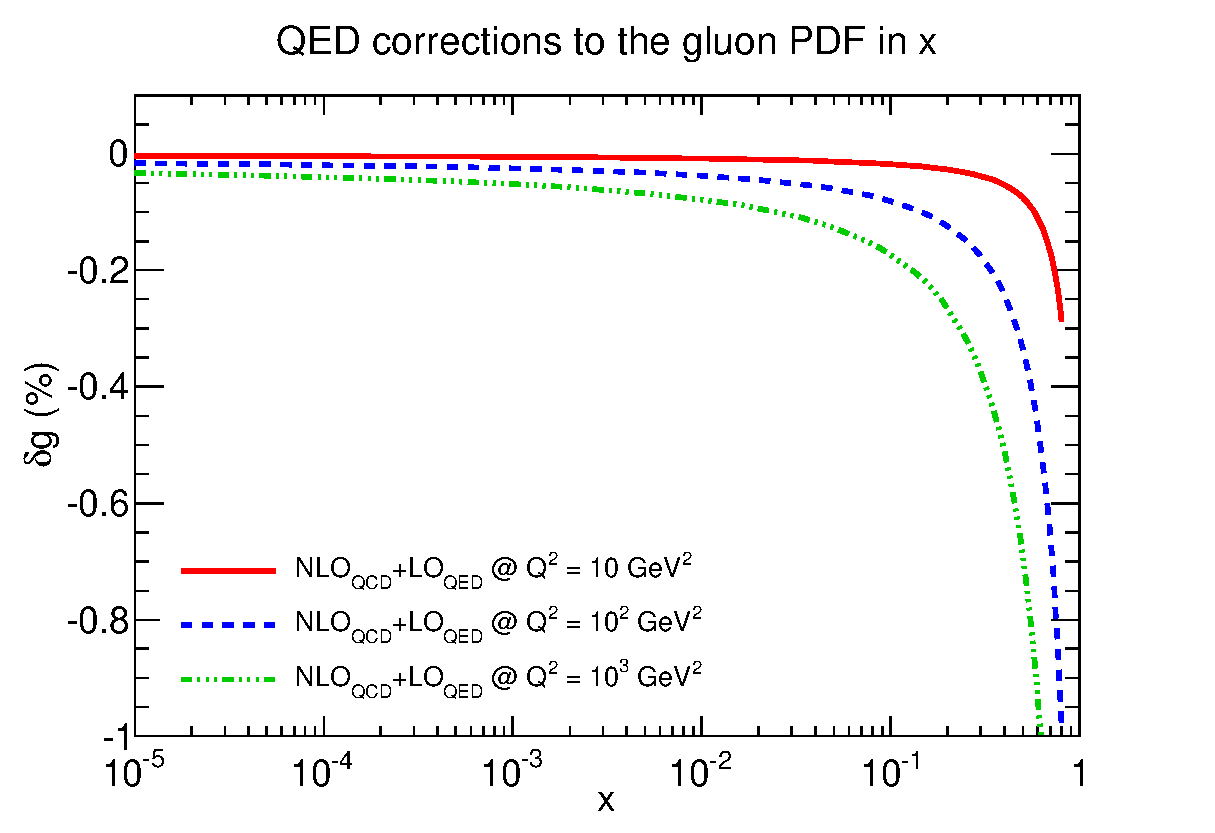
\includegraphics[scale=0.45]{plots/gluon}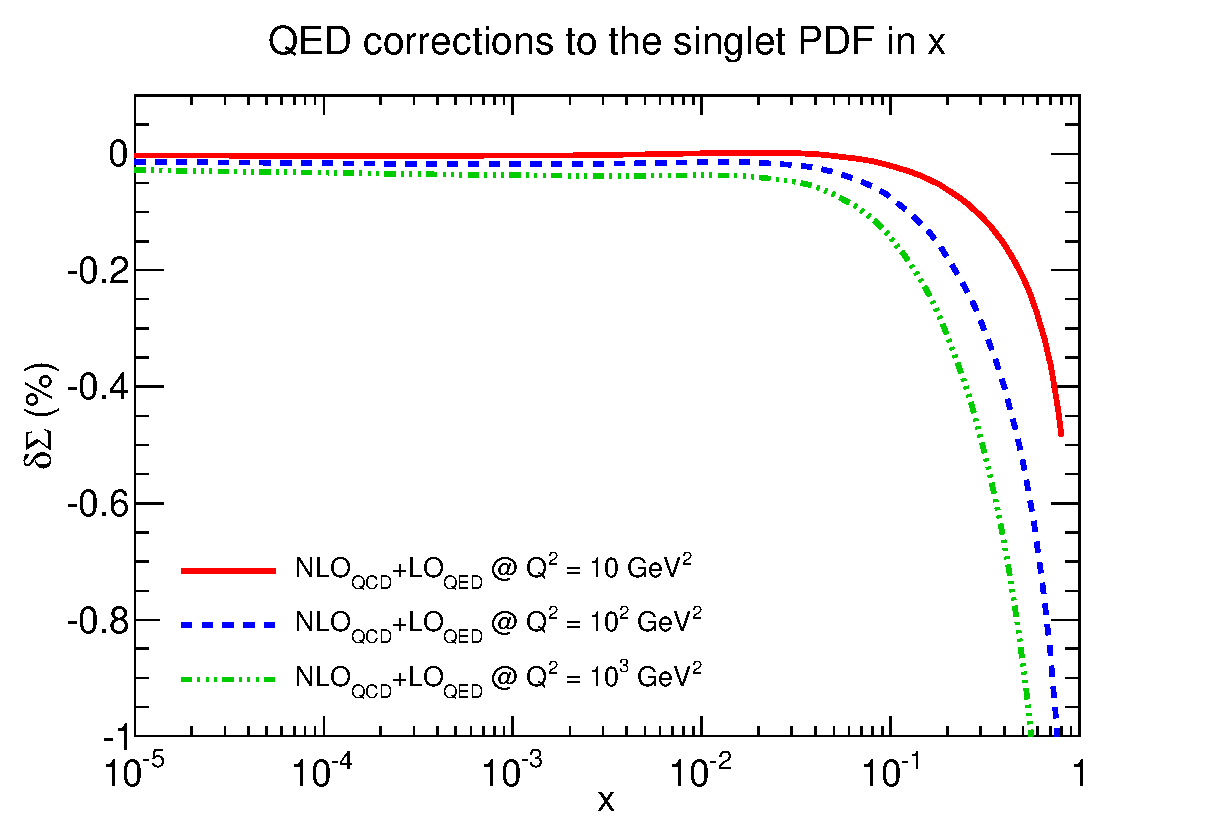
\includegraphics[scale=0.45]{plots/singlet}
\par\end{centering}

\begin{centering}
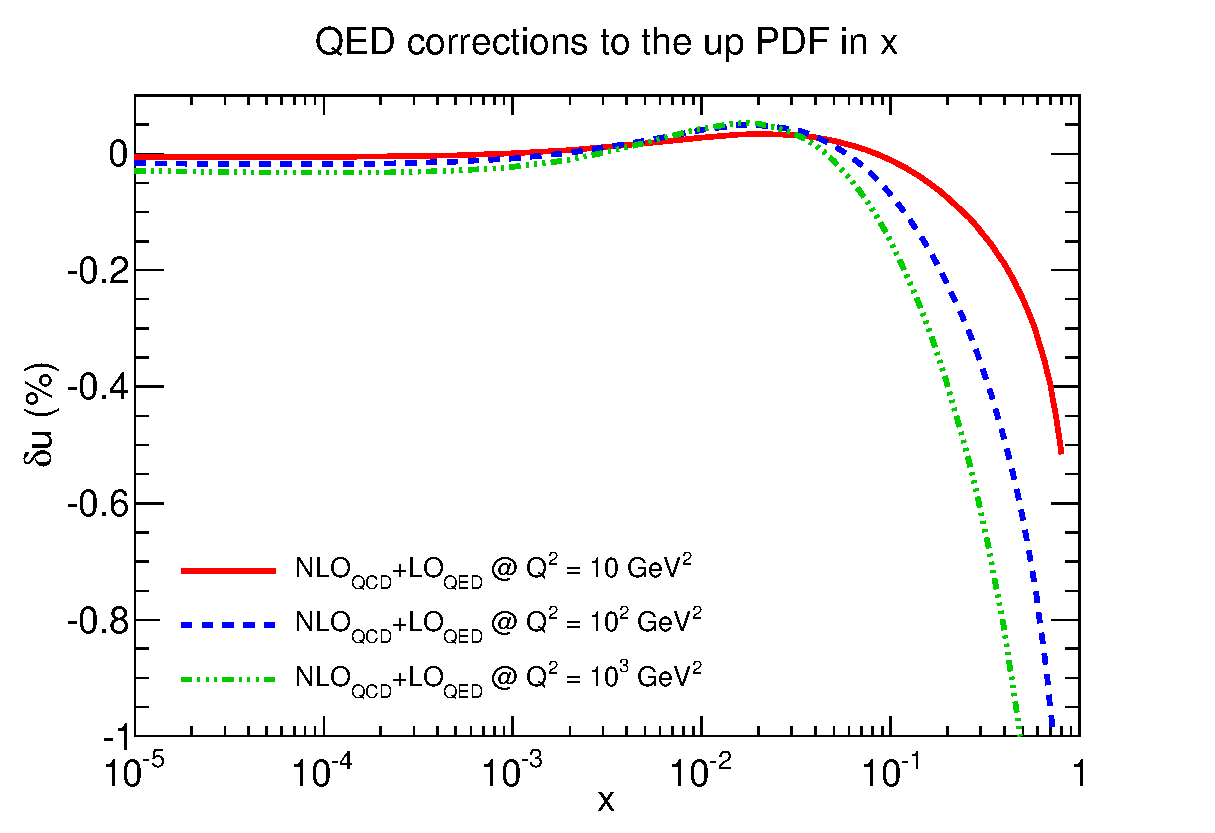
\includegraphics[scale=0.45]{plots/u}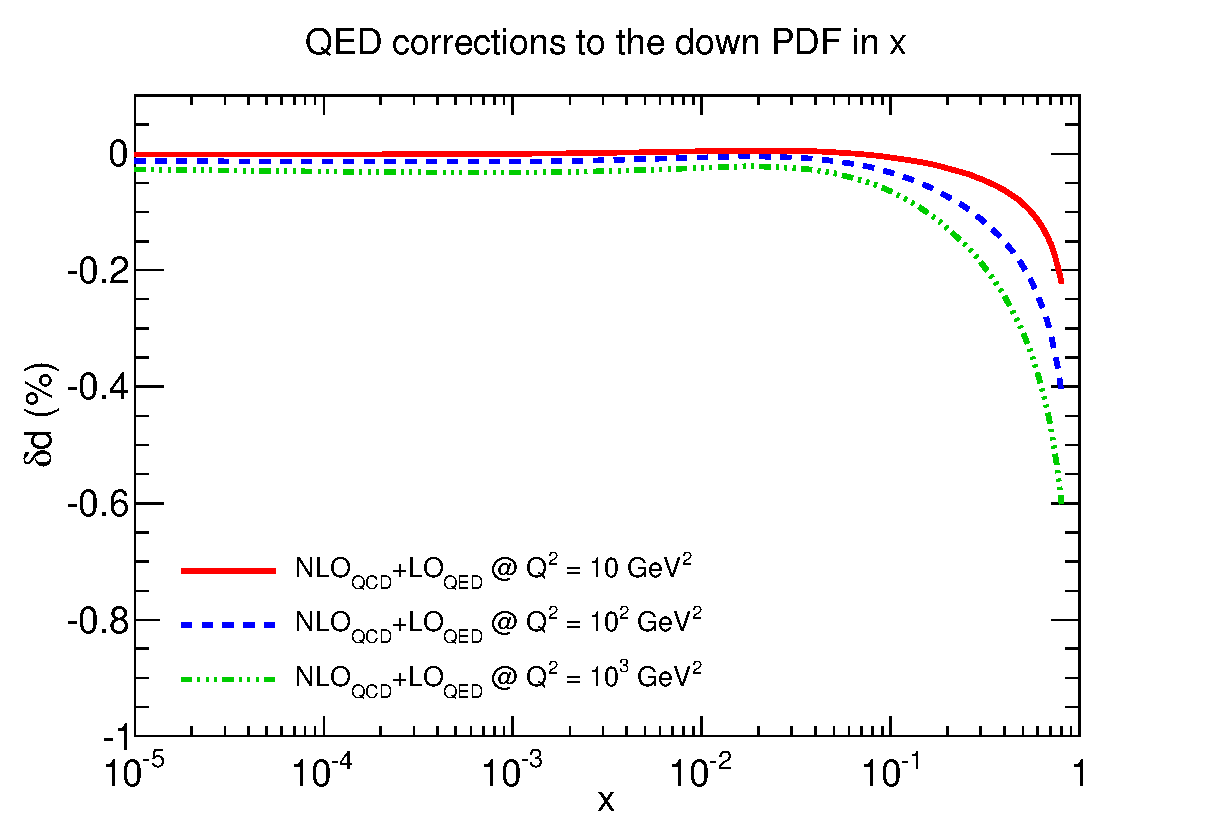
\includegraphics[scale=0.45]{plots/d}
\par\end{centering}

\begin{centering}
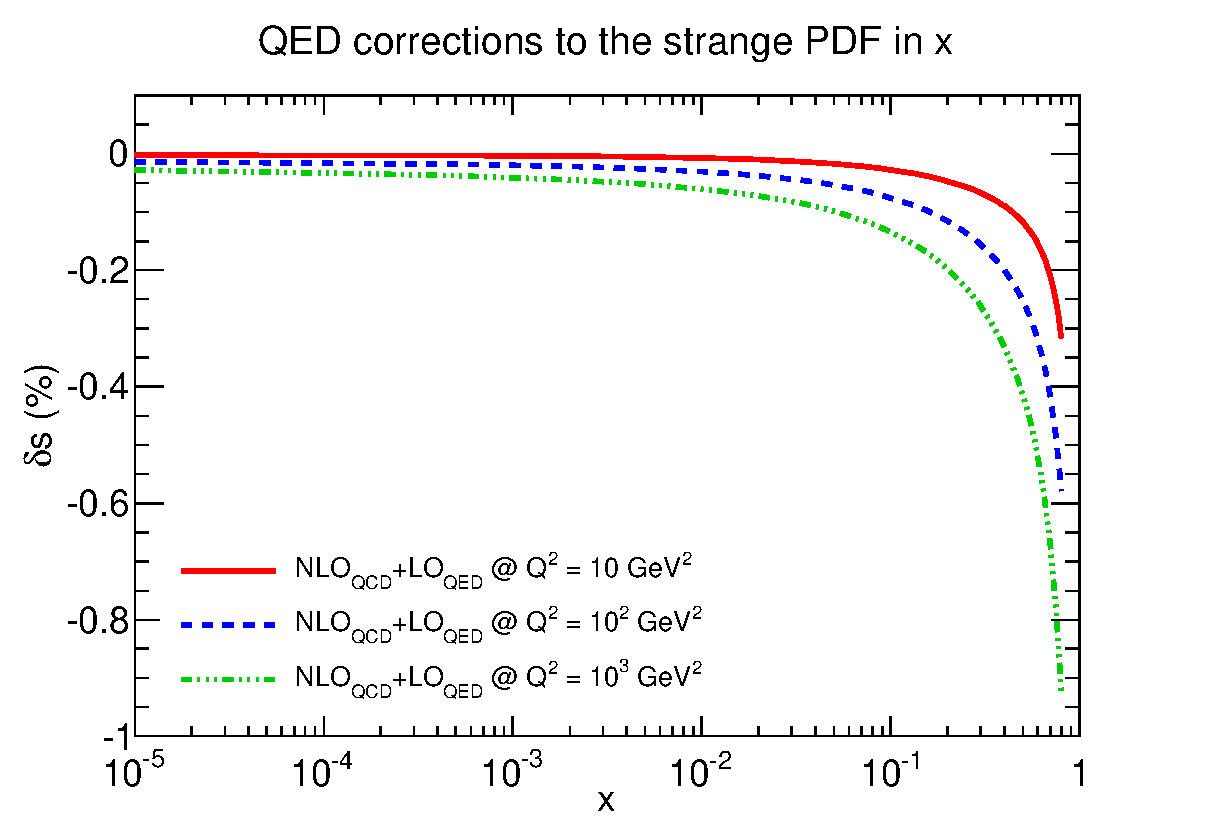
\includegraphics[scale=0.45]{plots/s}
\par\end{centering}

\caption{\label{fig:Impact-of-QED-figure}Impact of QED correction for $g,u,d,s,\Sigma$
PDFs. $x\gamma(x,Q_{0}^{2})=0$.}
\end{figure}


\begin{figure}
\begin{centering}
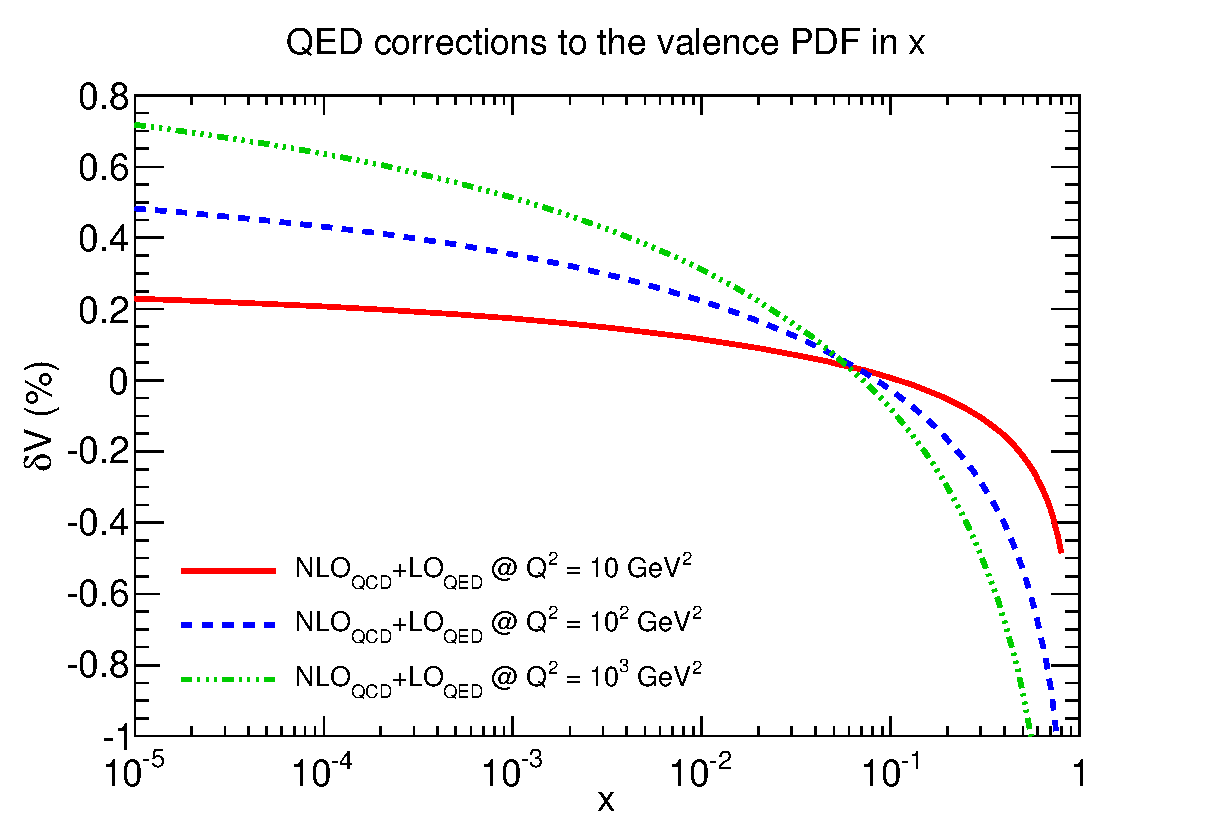
\includegraphics[scale=0.45]{plots/val}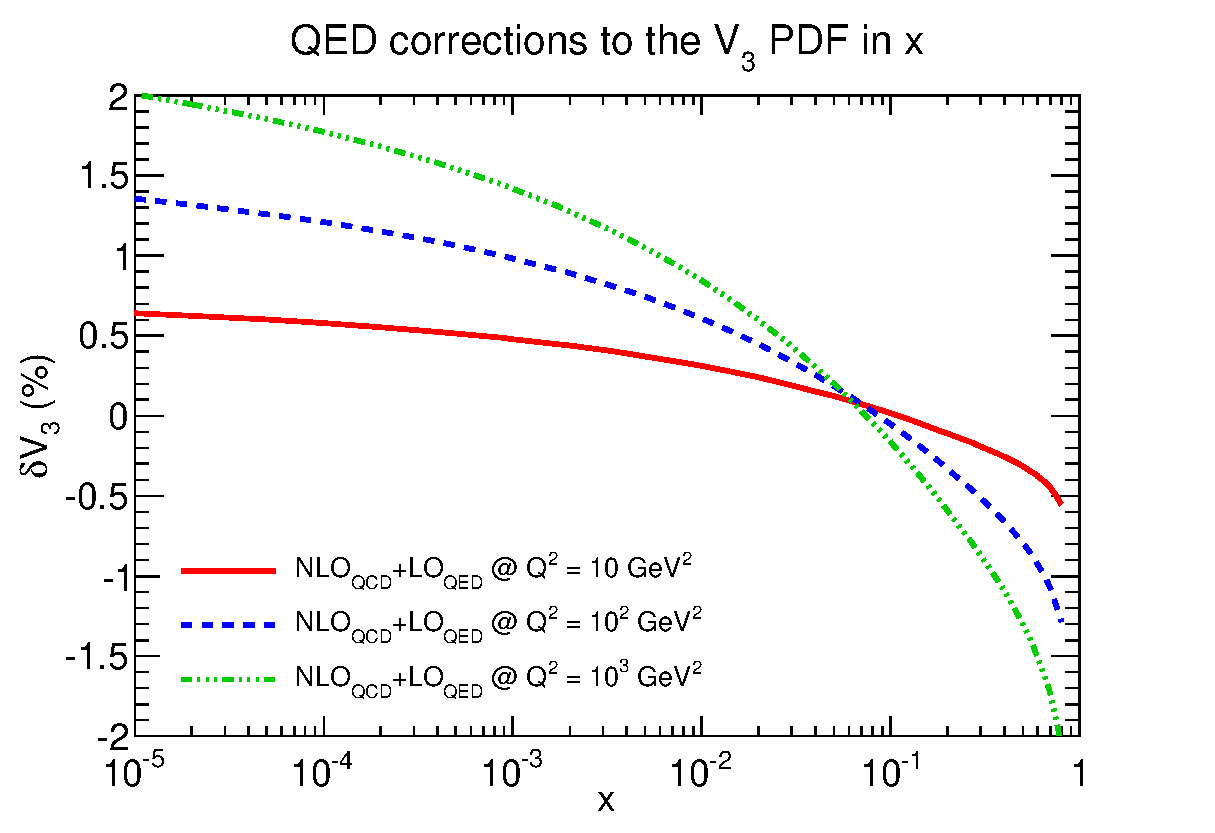
\includegraphics[scale=0.45]{plots/v03}
\par\end{centering}

\begin{centering}
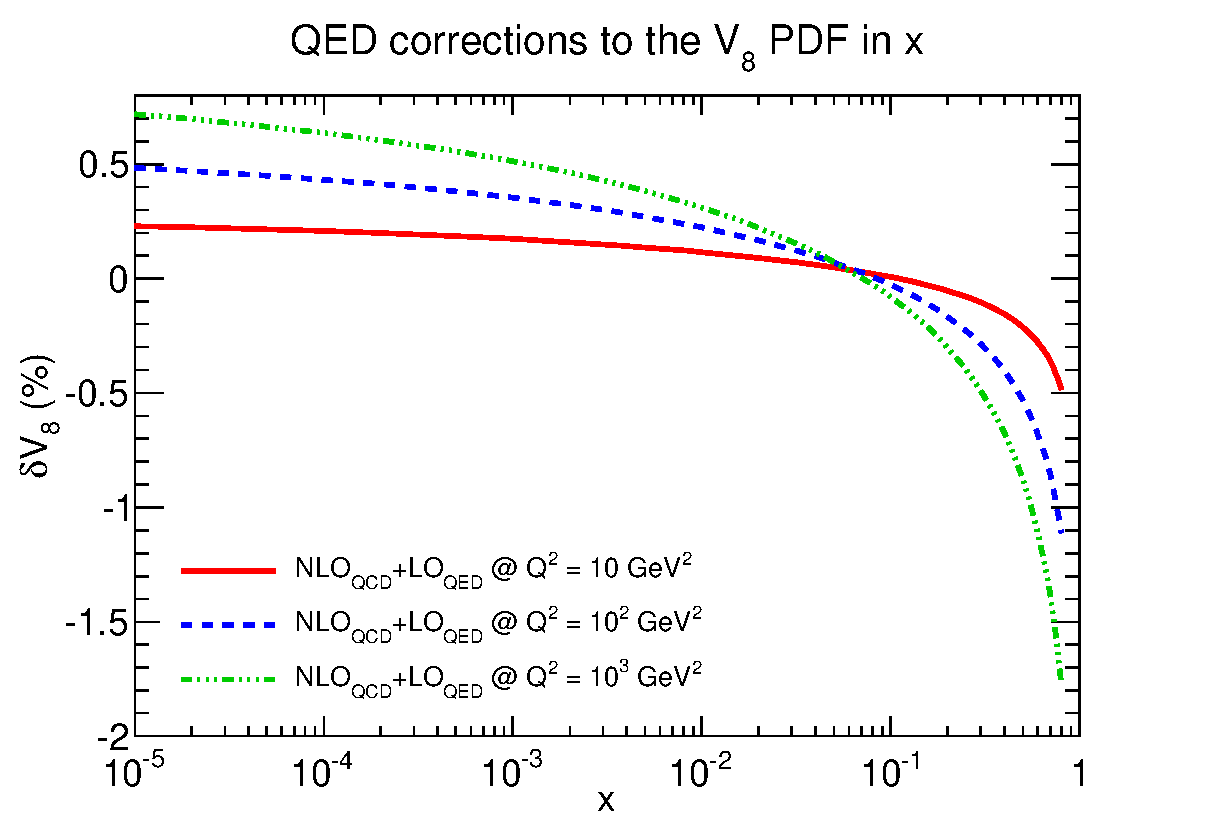
\includegraphics[scale=0.45]{plots/v08}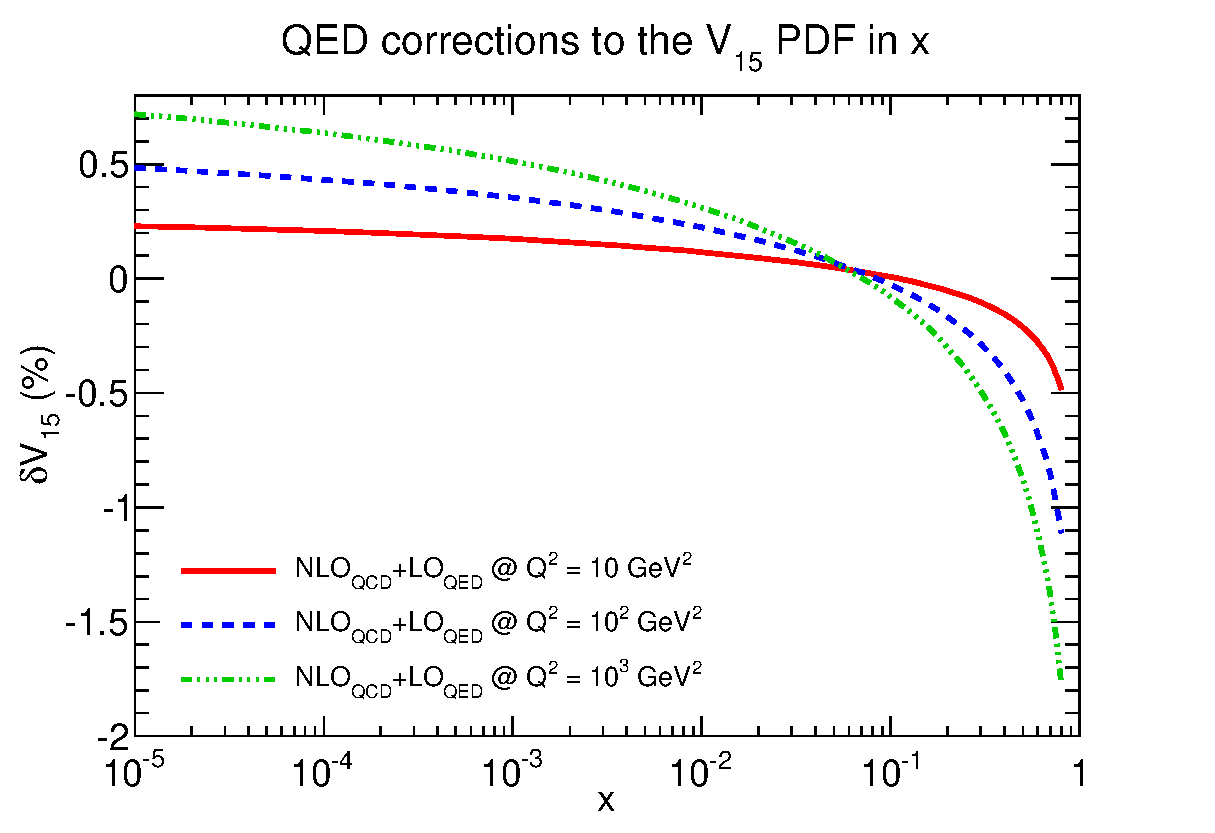
\includegraphics[scale=0.45]{plots/v15}
\par\end{centering}

\begin{centering}
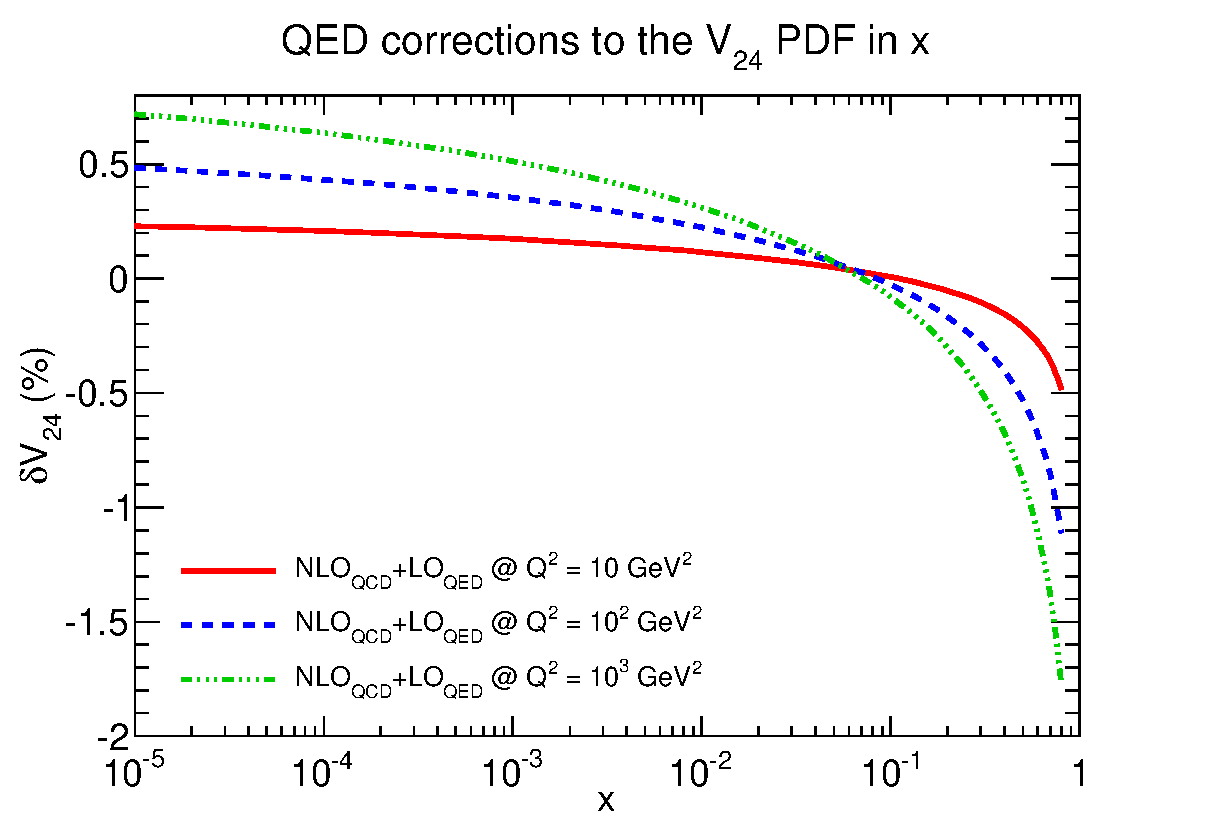
\includegraphics[scale=0.45]{plots/v24}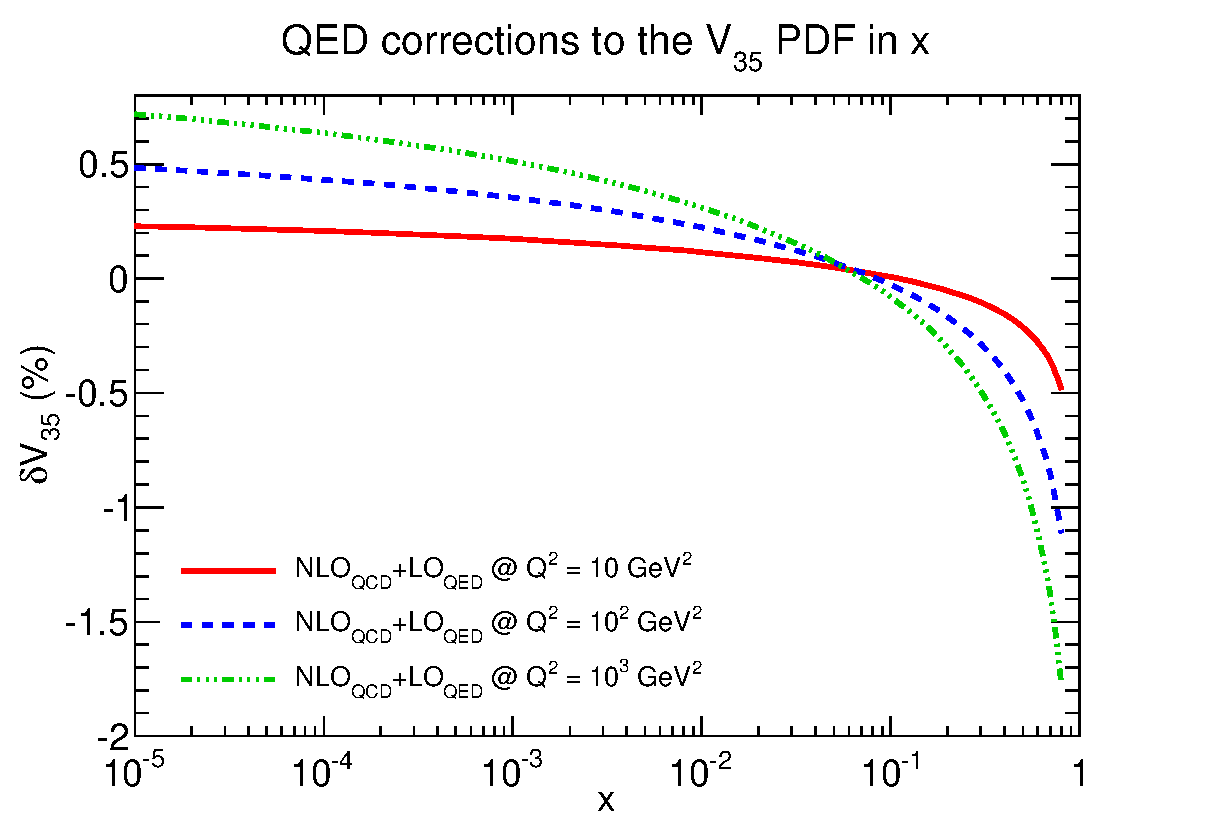
\includegraphics[scale=0.45]{plots/v35}
\par\end{centering}

\caption{\label{fig:Impact-of-QED-figure-2}Impact of QED correction for the
valence family. $x\gamma(x,Q_{0}^{2})=0$}
\end{figure}


\begin{figure}
\begin{centering}
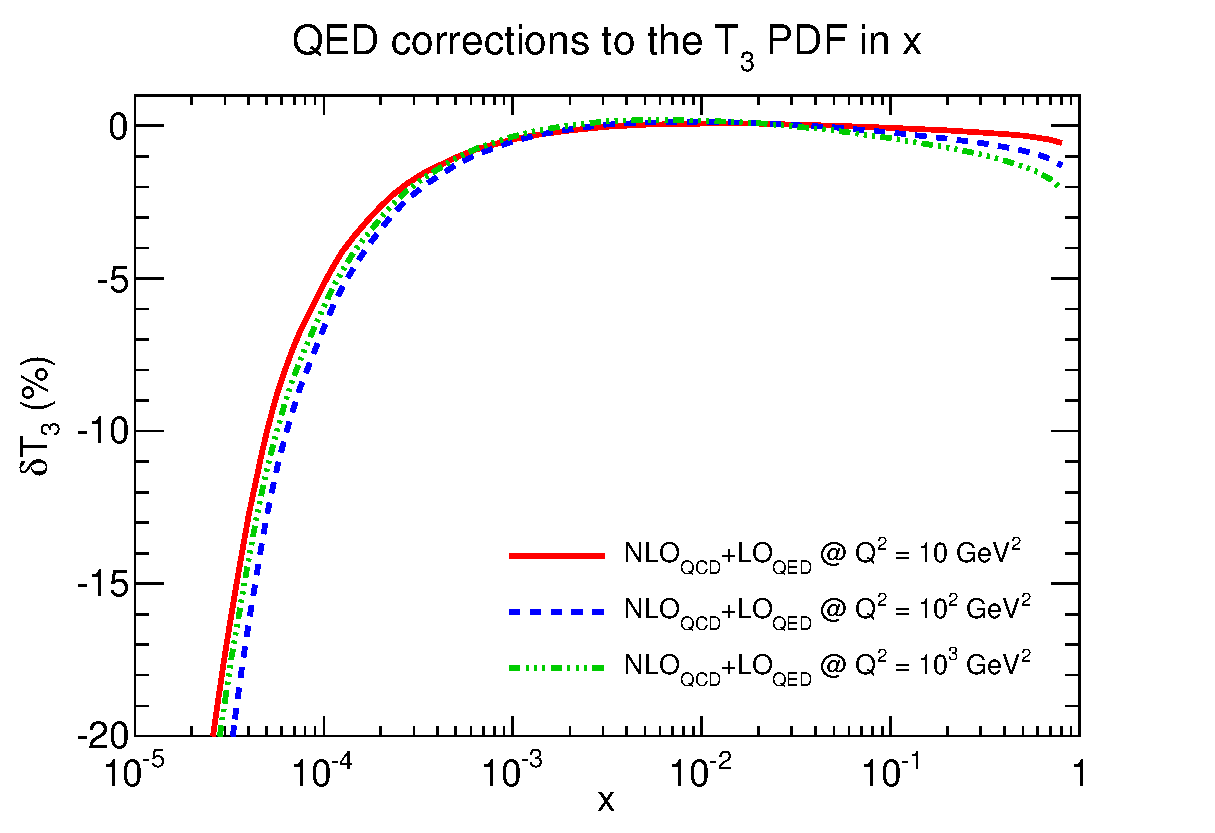
\includegraphics[scale=0.45]{plots/t03}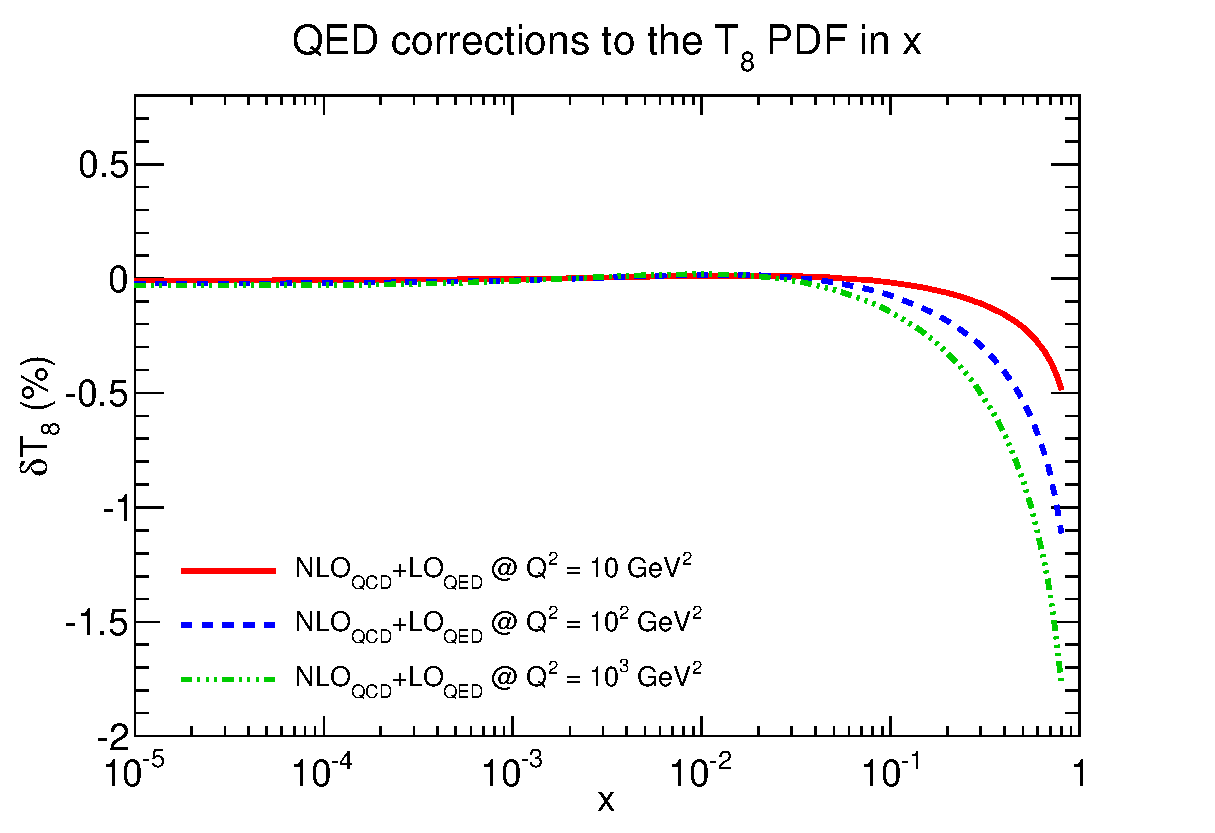
\includegraphics[scale=0.45]{plots/t08}
\par\end{centering}

\begin{centering}
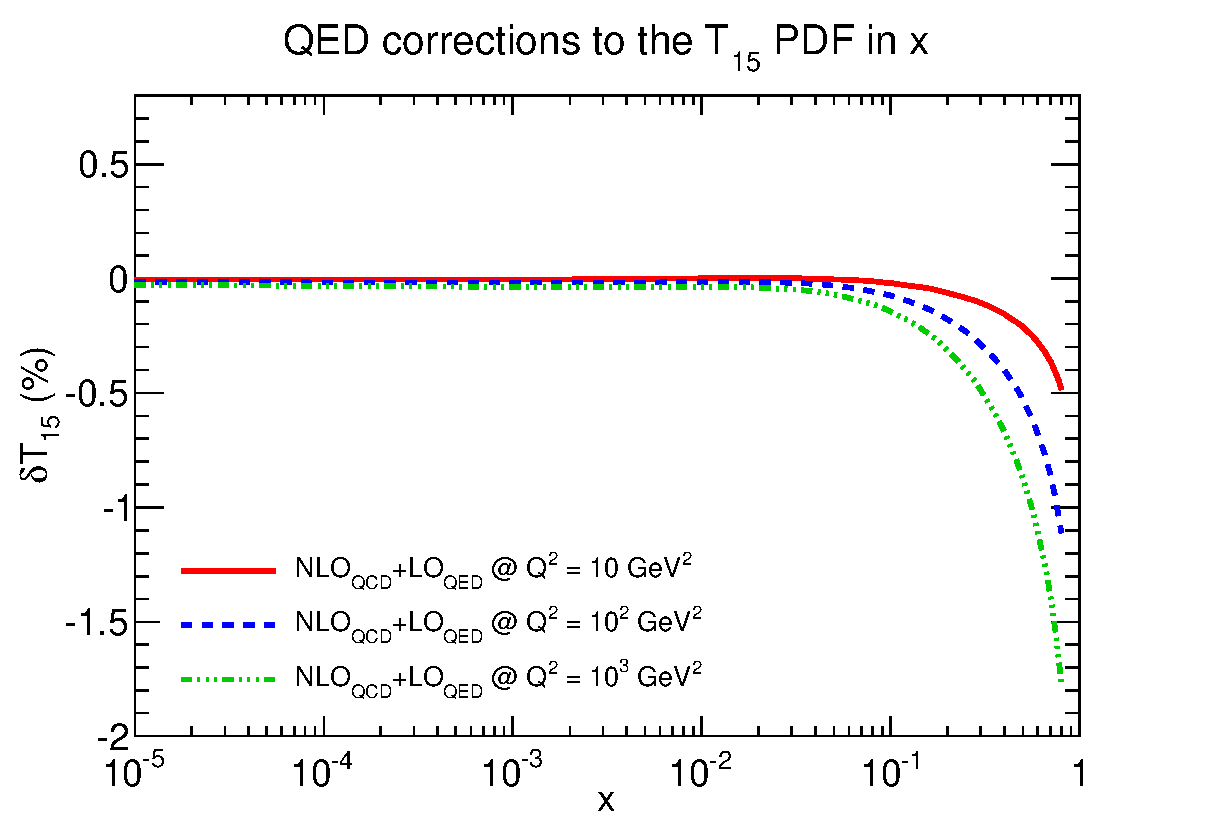
\includegraphics[scale=0.45]{plots/t15}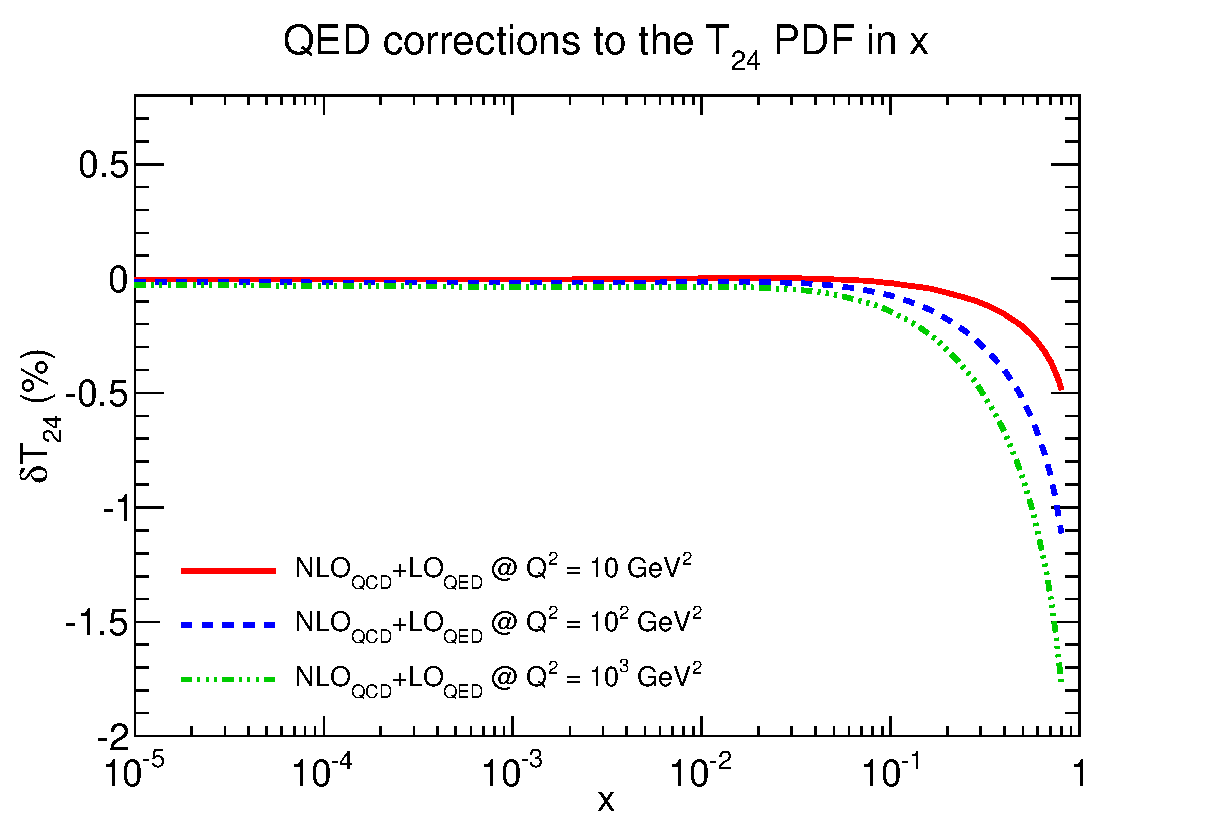
\includegraphics[scale=0.45]{plots/t24}
\par\end{centering}

\begin{centering}
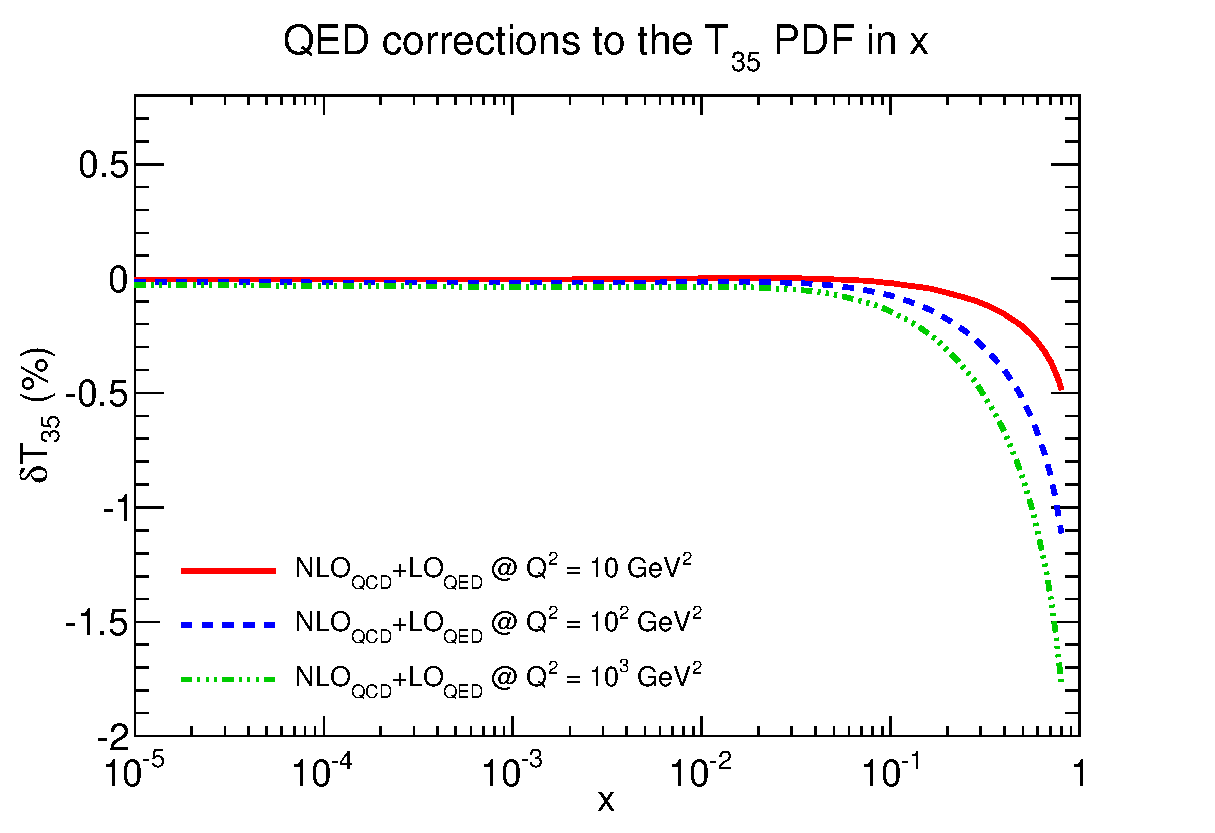
\includegraphics[scale=0.45]{plots/t35}
\par\end{centering}

\caption{\label{fig:Impact-of-QED-figure-3}Impact of QED correction for the
$T$ family. $x\gamma(x,Q_{0}^{2})=0$}
\end{figure}


\begin{table}
\begin{centering}
\subfloat[From $Q_{0}^{2}=2\,\text{GeV}^{2}$ to $Q^{2}=10\,\text{GeV}^{2}$]{\begin{centering}
\begin{tabular}{|c|c|c|c|c|c|c|c|c|}
\hline 
$x$  & $10^{-5}$  & $10^{-4}$  & $10^{-3}$  & $10^{-2}$  & $10^{-1}$  & $0.3$  & $0.7$ & $0.8$\tabularnewline
\hline 
\hline 
$\delta g$ (\%)  &  &  &  &  &  &  &  & \tabularnewline
\hline 
$\delta\Sigma$ (\%)  &  &  &  &  &  &  &  & \tabularnewline
\hline 
$\delta u$ (\%)  &  &  &  &  &  &  &  & \tabularnewline
\hline 
$\delta d$ (\%)  &  &  &  &  &  &  &  & \tabularnewline
\hline 
$\delta s$ (\%)  &  &  &  &  &  &  &  & \tabularnewline
\hline 
$\delta V$ (\%)  &  &  &  &  &  &  &  & \tabularnewline
\hline 
$\delta V_{3}$ (\%)  &  &  &  &  &  &  &  & \tabularnewline
\hline 
$\delta V_{8}$ (\%)  &  &  &  &  &  &  &  & \tabularnewline
\hline 
$\delta V_{15}$ (\%)  &  &  &  &  &  &  &  & \tabularnewline
\hline 
$\delta T_{3}$ (\%)  &  &  &  &  &  &  &  & \tabularnewline
\hline 
$\delta T_{8}$ (\%)  &  &  &  &  &  &  &  & \tabularnewline
\hline 
$\delta T_{15}$ (\%)  &  &  &  &  &  &  &  & \tabularnewline
\hline 
\end{tabular}
\par\end{centering}

}
\par\end{centering}

\begin{centering}
\subfloat[From $Q_{0}^{2}=2\,\text{GeV}^{2}$ to $Q^{2}=100\,\text{GeV}^{2}$.]{\begin{centering}
\begin{tabular}{|c|c|c|c|c|c|c|c|c|}
\hline 
$x$  & $10^{-5}$  & $10^{-4}$  & $10^{-3}$  & $10^{-2}$  & $10^{-1}$  & $0.3$  & $0.7$ & $0.8$\tabularnewline
\hline 
\hline 
$\delta g$ (\%)  &  &  &  &  &  &  &  & \tabularnewline
\hline 
$\delta\Sigma$ (\%)  &  &  &  &  &  &  &  & \tabularnewline
\hline 
$\delta u$ (\%)  &  &  &  &  &  &  &  & \tabularnewline
\hline 
$\delta d$ (\%)  &  &  &  &  &  &  &  & \tabularnewline
\hline 
$\delta s$ (\%)  &  &  &  &  &  &  &  & \tabularnewline
\hline 
$\delta V$ (\%)  &  &  &  &  &  &  &  & \tabularnewline
\hline 
$\delta V_{3}$ (\%)  &  &  &  &  &  &  &  & \tabularnewline
\hline 
$\delta V_{8}$ (\%)  &  &  &  &  &  &  &  & \tabularnewline
\hline 
$\delta V_{15}$ (\%)  &  &  &  &  &  &  &  & \tabularnewline
\hline 
$\delta T_{3}$ (\%)  &  &  &  &  &  &  &  & \tabularnewline
\hline 
$\delta T_{8}$ (\%)  &  &  &  &  &  &  &  & \tabularnewline
\hline 
$\delta T_{15}$ (\%)  &  &  &  &  &  &  &  & \tabularnewline
\hline 
\end{tabular}
\par\end{centering}

}
\par\end{centering}

\begin{centering}
\subfloat[From $Q_{0}^{2}=2\,\text{GeV}^{2}$ to $Q^{2}=1000\,\text{GeV}^{2}$.]{\begin{centering}
\begin{tabular}{|c|c|c|c|c|c|c|c|c|}
\hline 
$x$  & $10^{-5}$  & $10^{-4}$  & $10^{-3}$  & $10^{-2}$  & $10^{-1}$  & $0.3$  & $0.7$ & $0.8$\tabularnewline
\hline 
\hline 
$\delta g$ (\%)  &  &  &  &  &  &  &  & \tabularnewline
\hline 
$\delta\Sigma$ (\%)  &  &  &  &  &  &  &  & \tabularnewline
\hline 
$\delta u$ (\%)  &  &  &  &  &  &  &  & \tabularnewline
\hline 
$\delta d$ (\%)  &  &  &  &  &  &  &  & \tabularnewline
\hline 
$\delta s$ (\%)  &  &  &  &  &  &  &  & \tabularnewline
\hline 
$\delta V$ (\%)  &  &  &  &  &  &  &  & \tabularnewline
\hline 
$\delta V_{3}$ (\%)  &  &  &  &  &  &  &  & \tabularnewline
\hline 
$\delta V_{8}$ (\%)  &  &  &  &  &  &  &  & \tabularnewline
\hline 
$\delta V_{15}$ (\%)  &  &  &  &  &  &  &  & \tabularnewline
\hline 
$\delta T_{3}$ (\%)  &  &  &  &  &  &  &  & \tabularnewline
\hline 
$\delta T_{8}$ (\%)  &  &  &  &  &  &  &  & \tabularnewline
\hline 
$\delta T_{15}$ (\%)  &  &  &  &  &  &  &  & \tabularnewline
\hline 
\end{tabular}
\par\end{centering}

}
\par\end{centering}

\caption{\label{tab:Relative-differences-table}Relative differences for evolution
with NLO QCD + LO QED. $x\gamma(x,Q_{0}^{2})=0$}
\end{table}


\begin{figure}
\begin{centering}
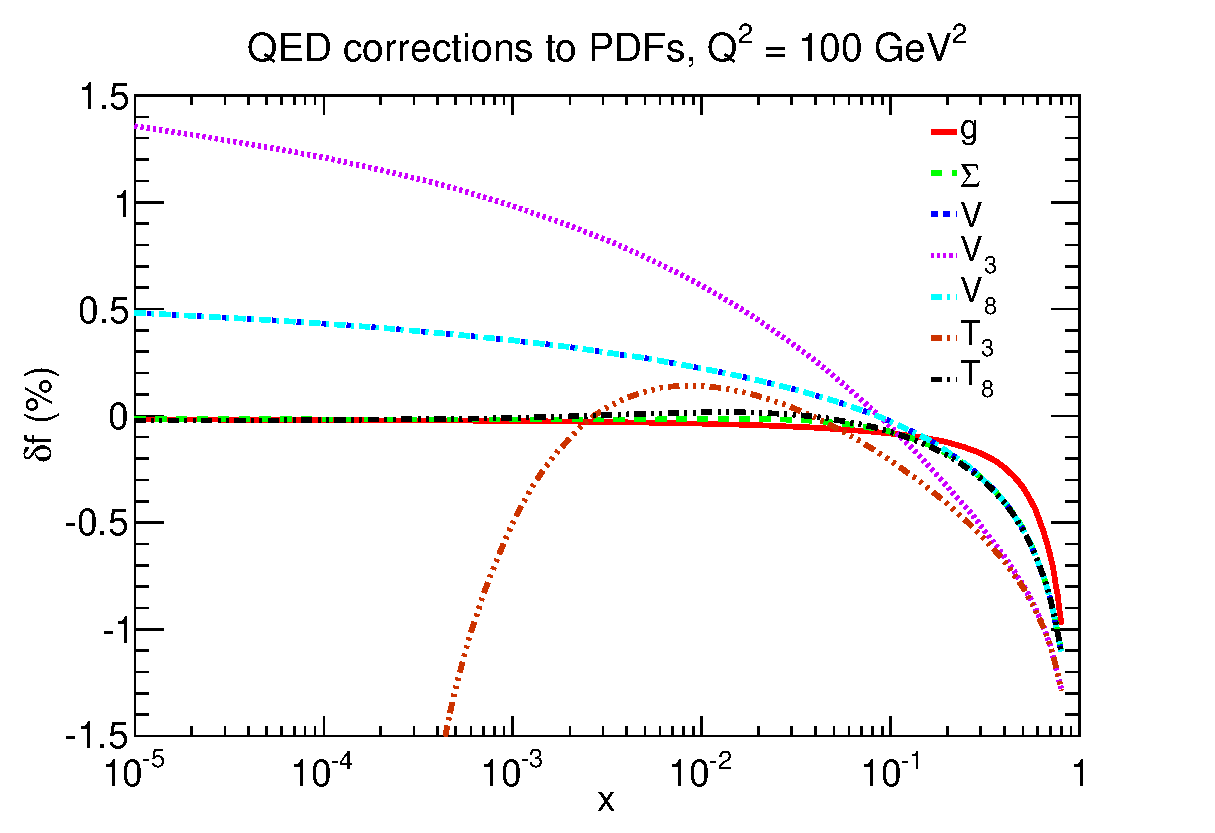
\includegraphics[scale=0.45]{plots/allPDFs}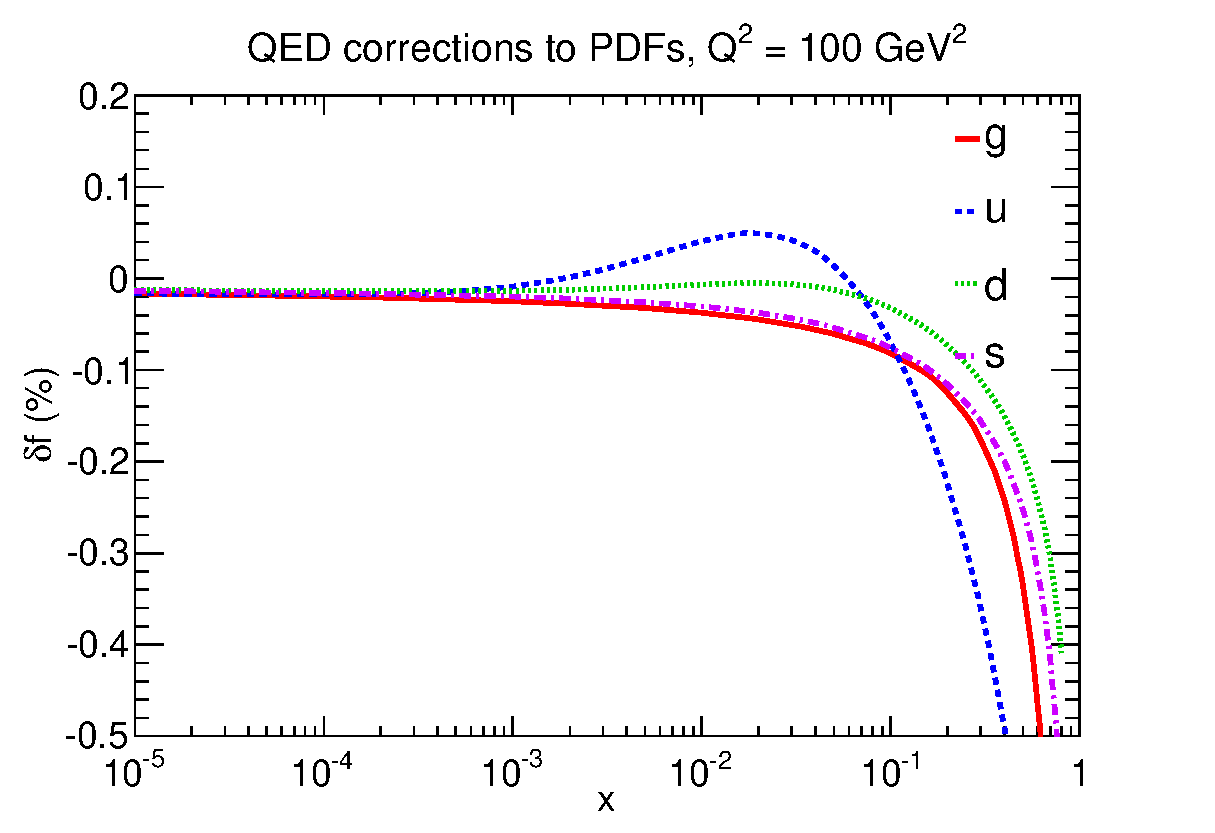
\includegraphics[scale=0.45]{plots/lhaPDFs}
\par\end{centering}

\begin{centering}
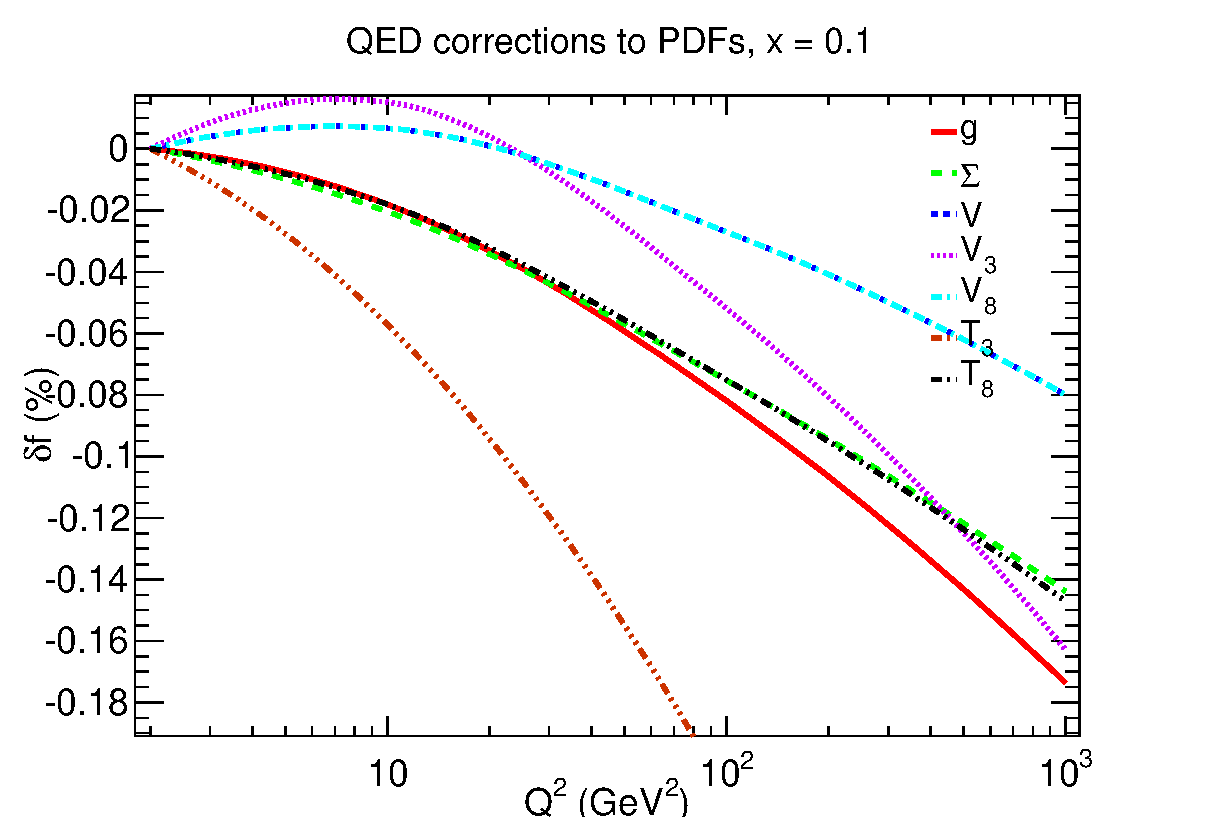
\includegraphics[scale=0.45]{plots/allPDFsQ}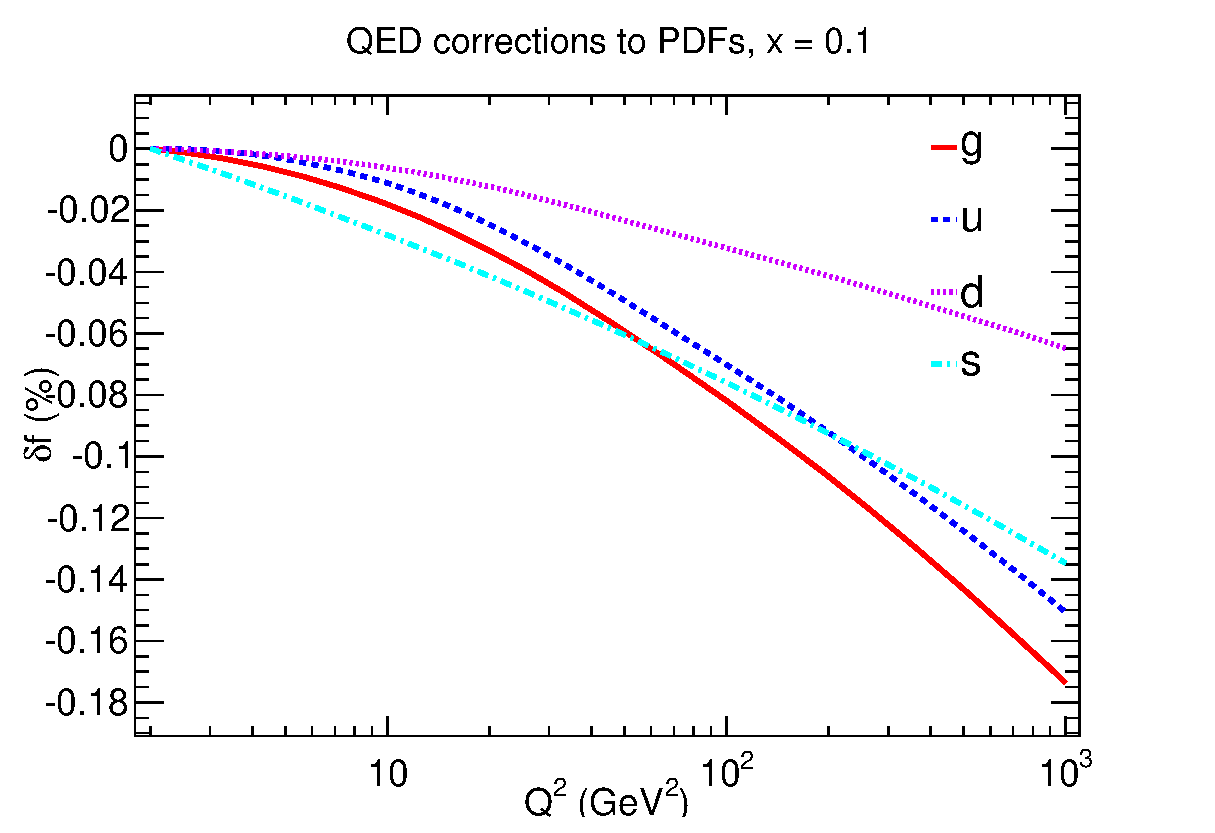
\includegraphics[scale=0.45]{plots/lhaPDFsQ}
\par\end{centering}

\caption{\label{fig:Summary-with-all}Summary with all PDFs together. $x\gamma(x,Q_{0}^{2})=0$}
\end{figure}


\newpage{}


\subsection{FFNS Initial condition $x\gamma(x,Q_{0}^{2})\propto xg(x,Q_{0}^{2})$}

Lets suppose now that $x\gamma(x,Q_{0}^{2})=\alpha/\alpha_{S}xg(x,Q_{0}^{2})$
at $Q_{0}^{2}=2\,\text{GeV}^{2}$, the relative difference between
PDFs evolved with NLO QCD and NLO QCD + LO QED is showed in: Figure
\ref{fig:Impact-of-QED-figure-1b} for the singlet sector, Figure
\ref{fig:Impact-of-QED-figure-2a} for the valence, and Figure \ref{fig:Impact-of-QED-figure-3a}
for the triplet.

We still observing differences of 1\% at high $x$ for the singlet
sector, and again, the triplet at is strongly modified at small-$x$.

Table \ref{tab:Relative-differences-table-2} illustrates for each
PDF the relative difference for specific $x$ values. Finally, Figure
\ref{fig:Summary-with-all-1b} shows the comparison between the relative
difference of all PDFs and the $Q^{2}$ dependence of the relative
ratio.

\begin{figure}[H]
\begin{centering}
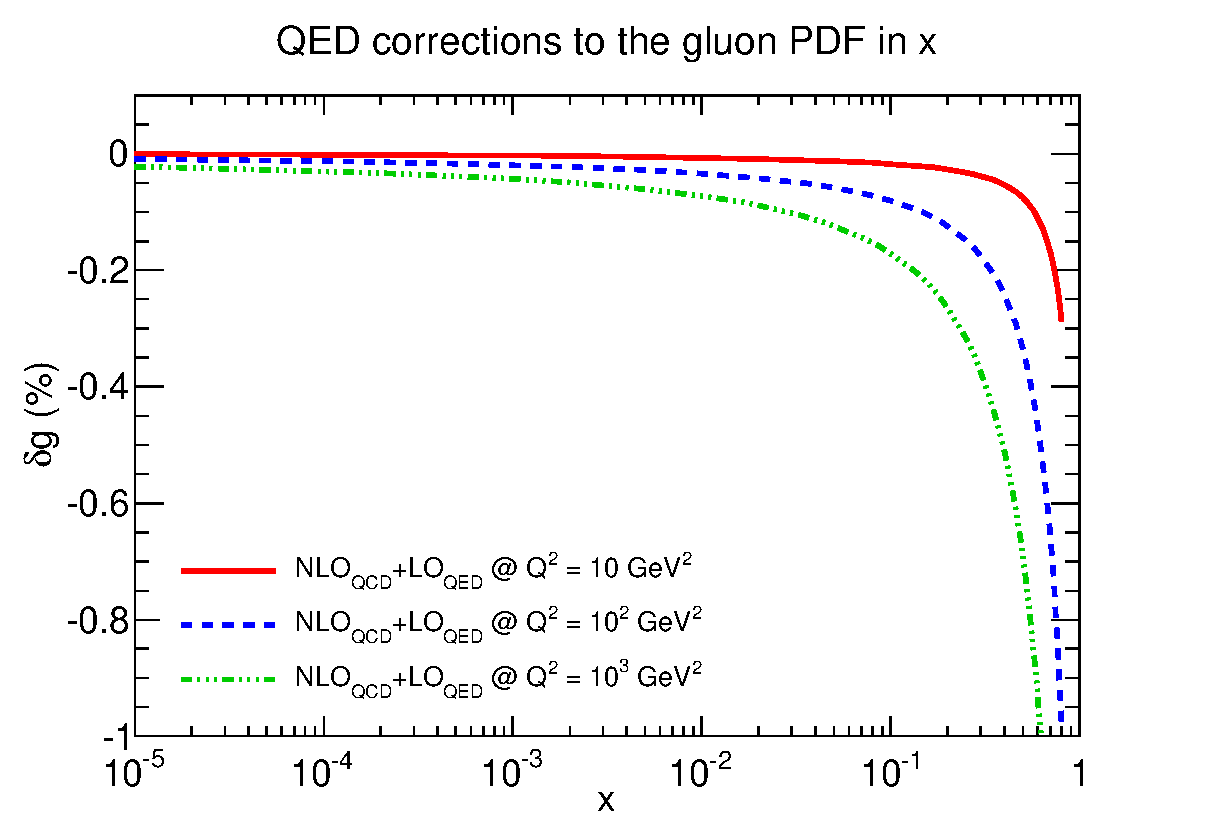
\includegraphics[scale=0.45]{plots/gluon_glike}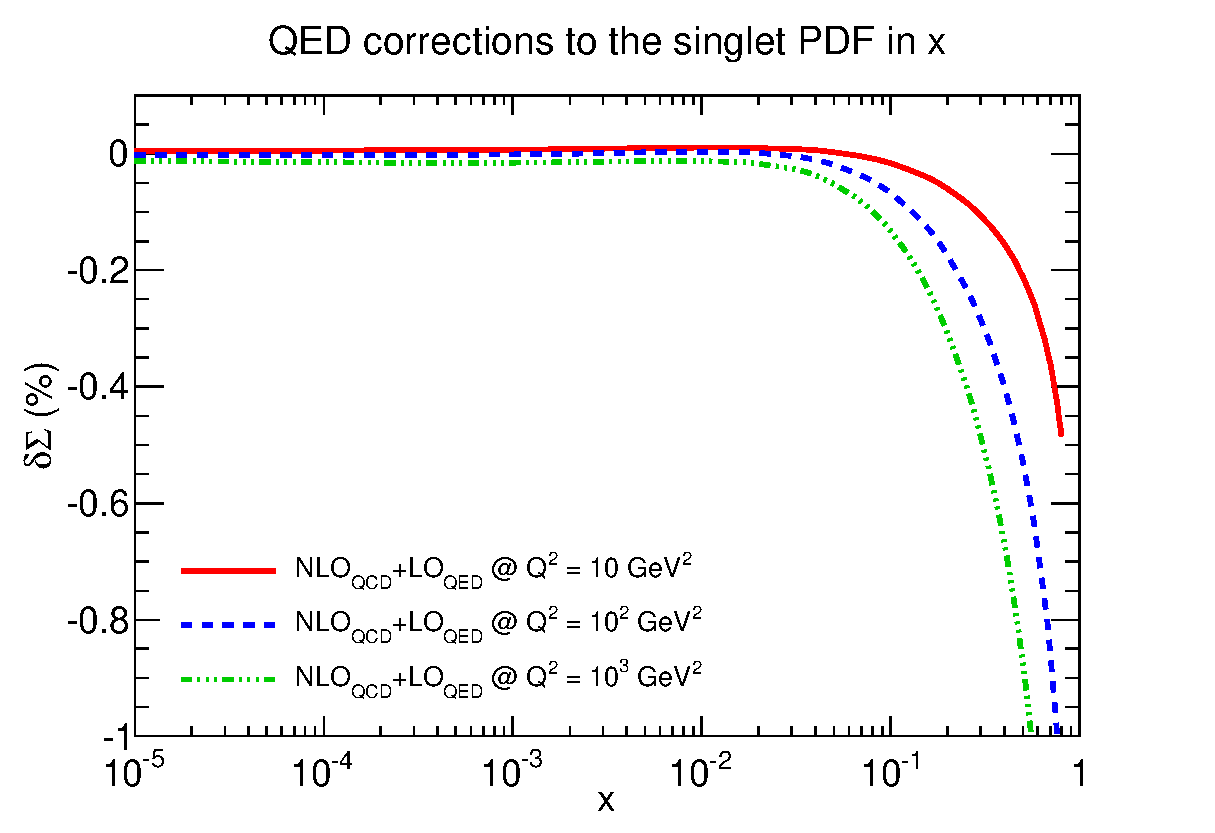
\includegraphics[scale=0.45]{plots/singlet_glike}
\par\end{centering}

\begin{centering}
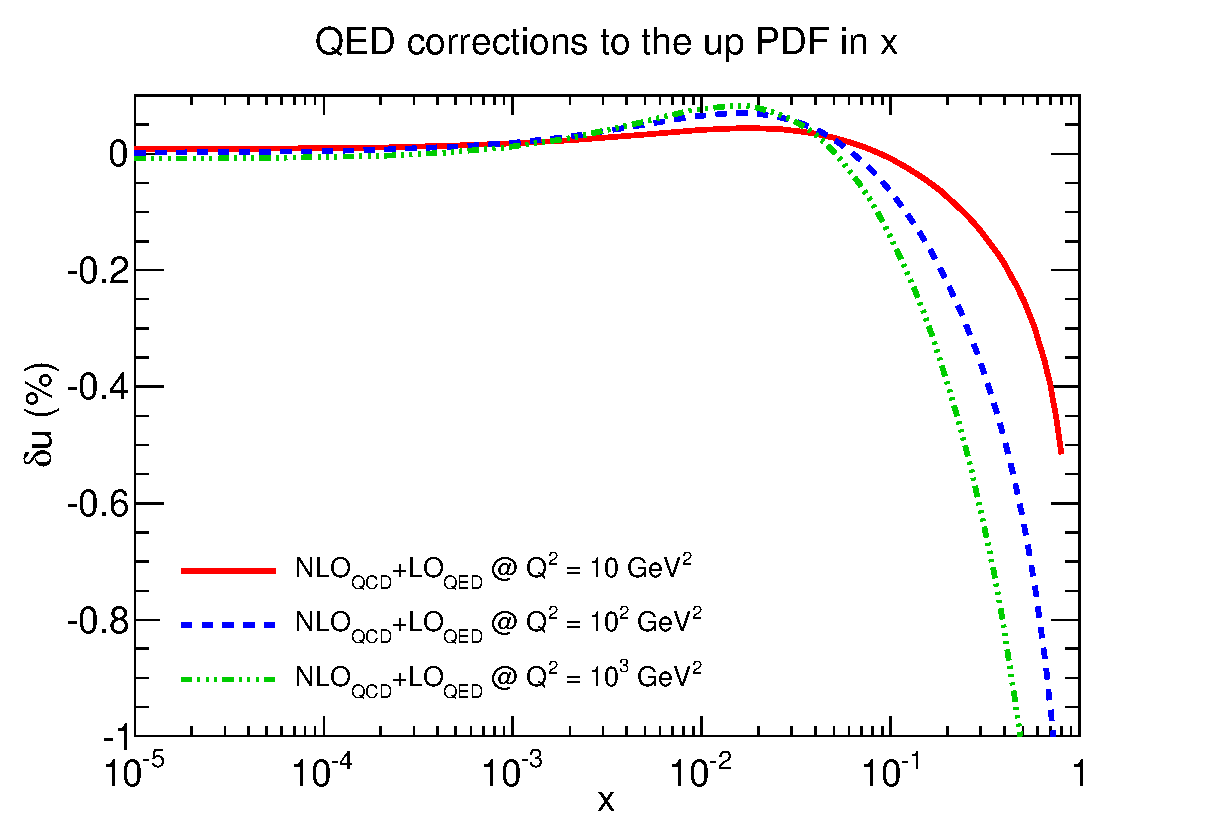
\includegraphics[scale=0.45]{plots/u_glike}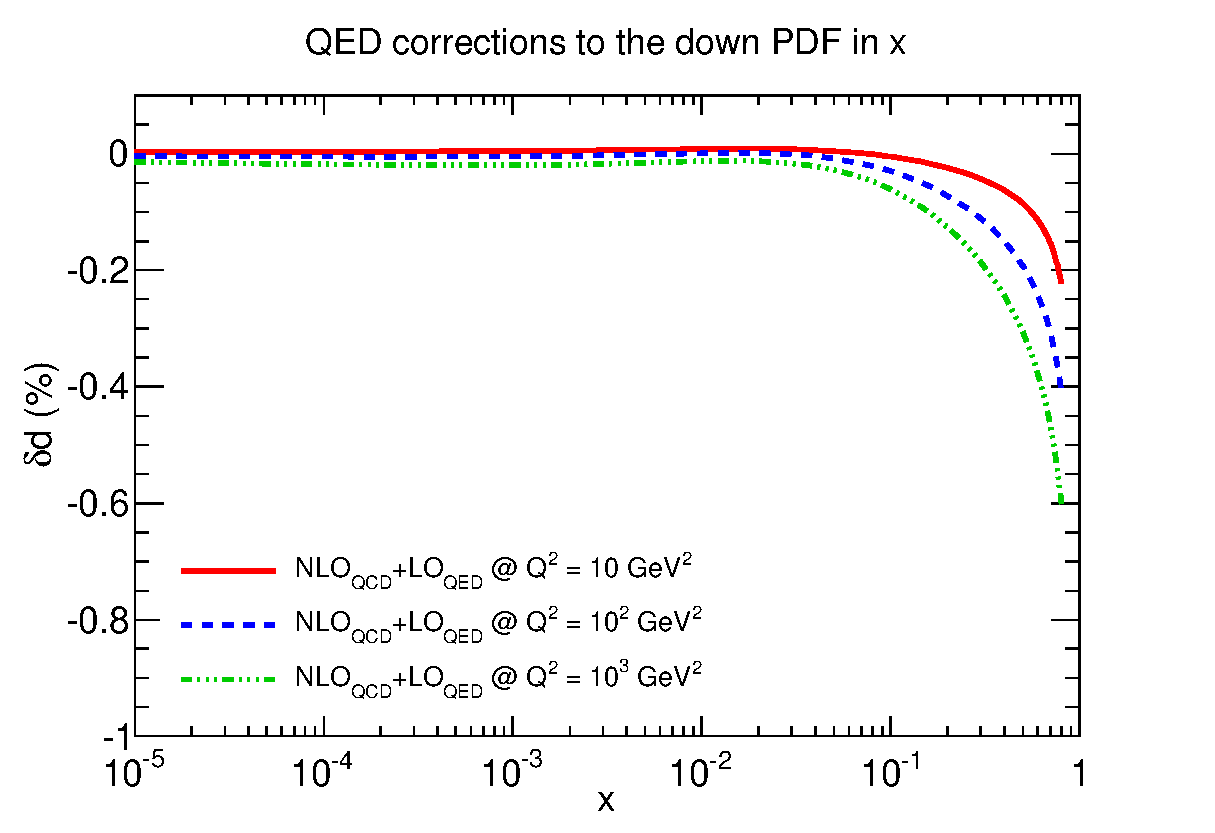
\includegraphics[scale=0.45]{plots/d_glike}
\par\end{centering}

\begin{centering}
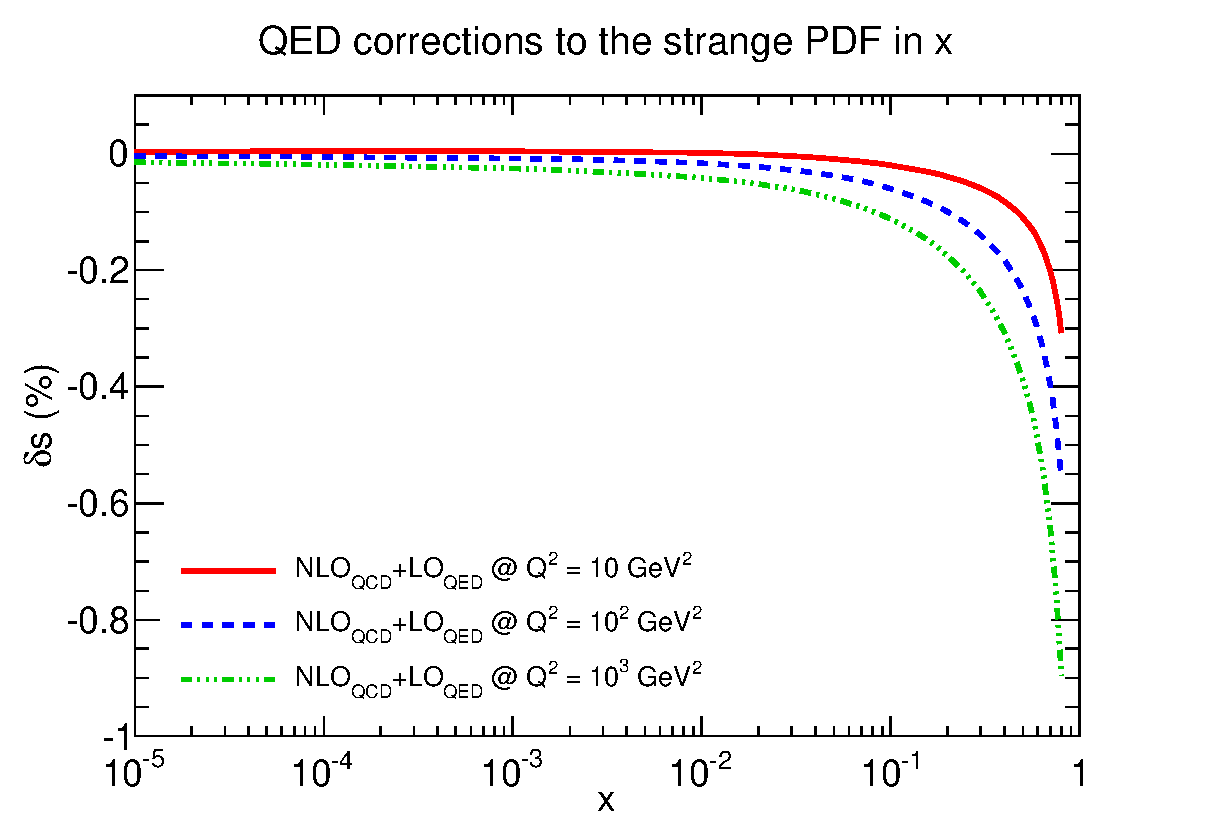
\includegraphics[scale=0.45]{plots/s_glike}
\par\end{centering}

\caption{\label{fig:Impact-of-QED-figure-1b}Impact of QED correction for $g,u,d,s,\Sigma$
PDFs. $x\gamma(x,Q_{0}^{2})=\alpha/\alpha_{S}xg(x,Q_{0}^{2})$}
\end{figure}


\begin{figure}
\begin{centering}
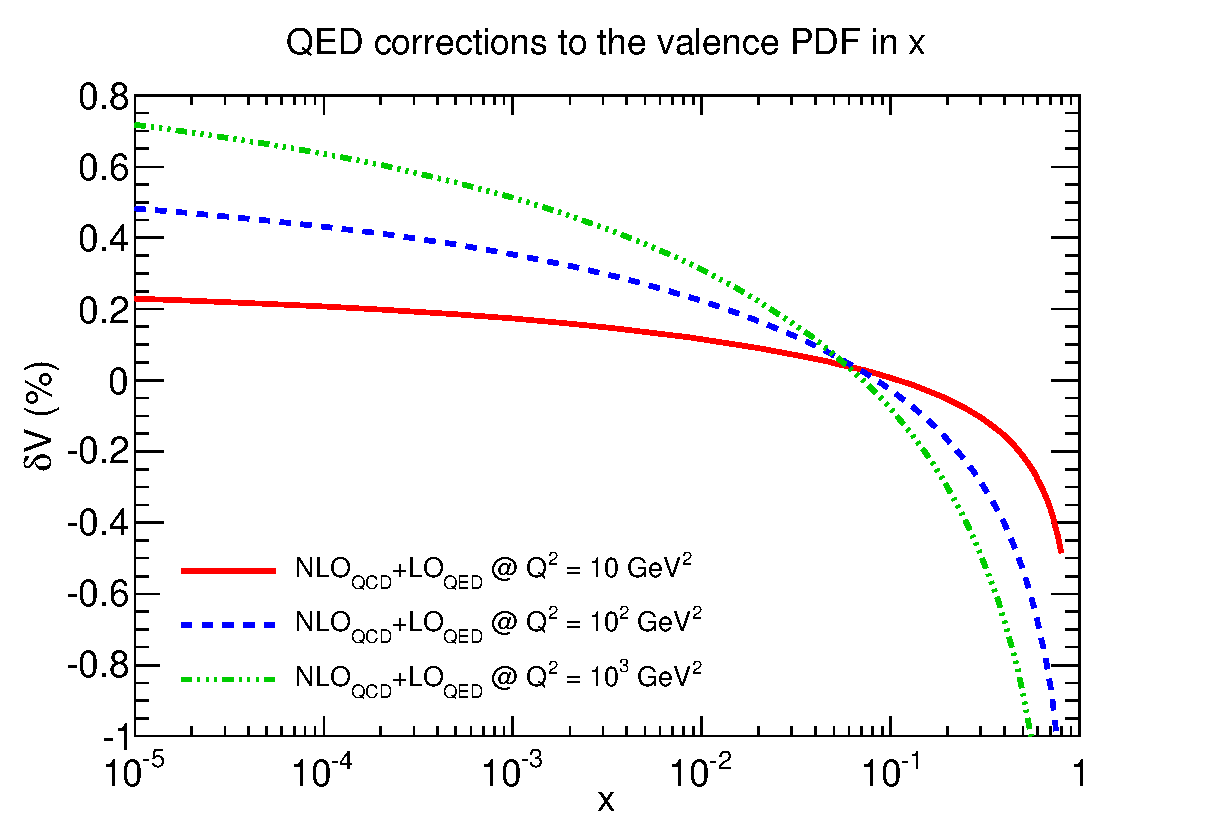
\includegraphics[scale=0.45]{plots/val_glike}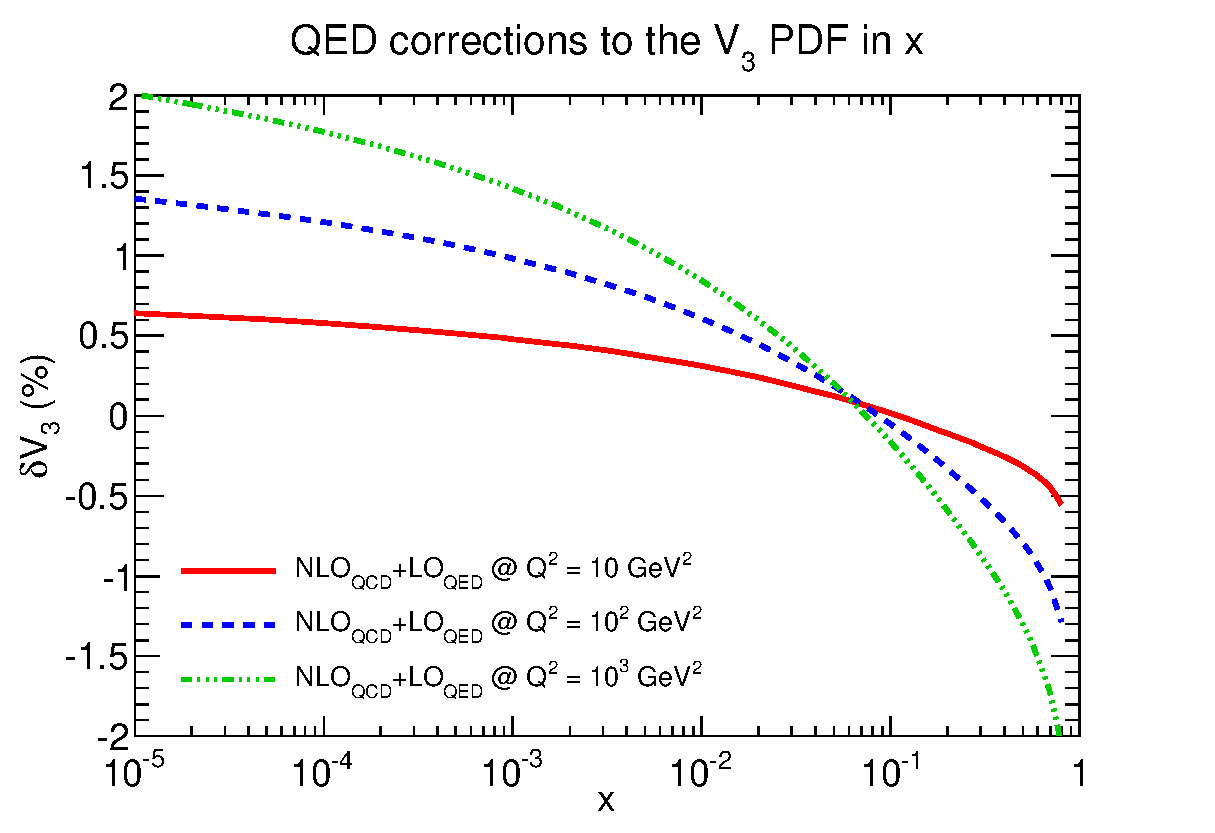
\includegraphics[scale=0.45]{plots/v03_glike}
\par\end{centering}

\begin{centering}
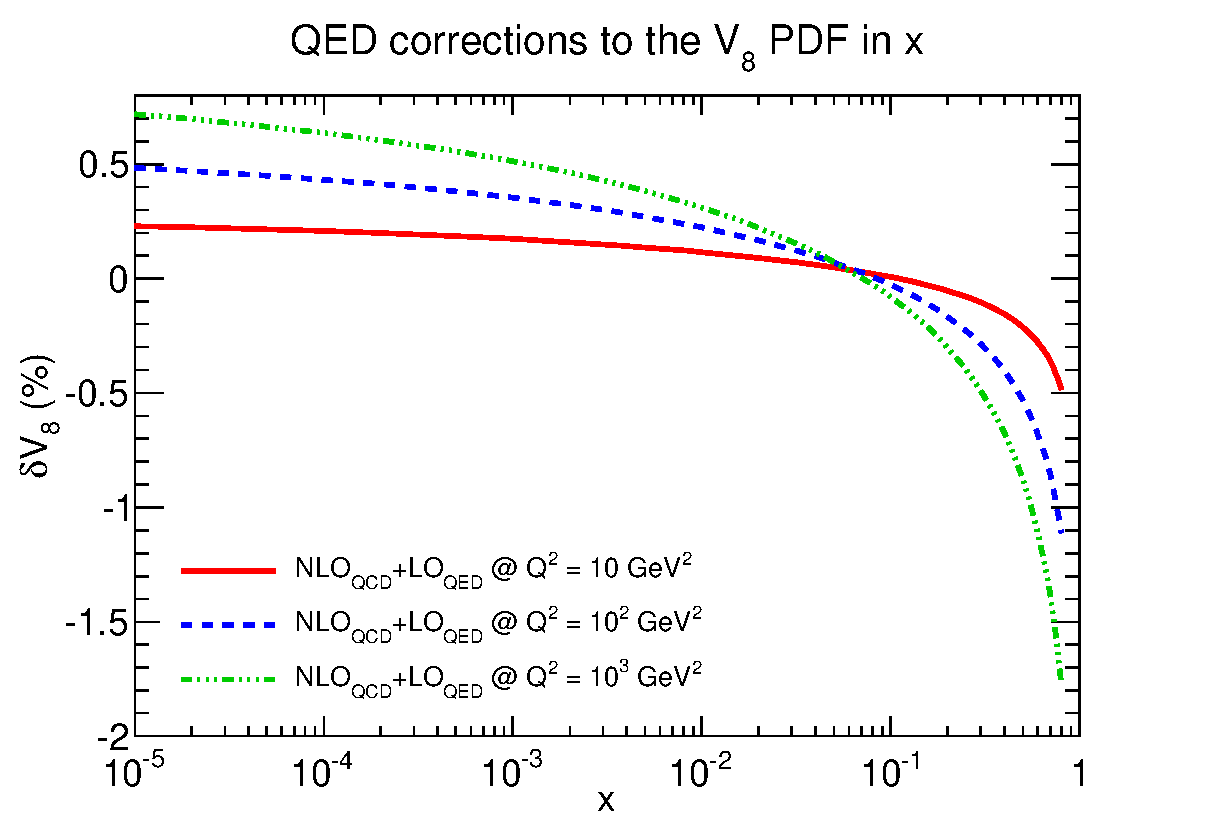
\includegraphics[scale=0.45]{plots/v08_glike}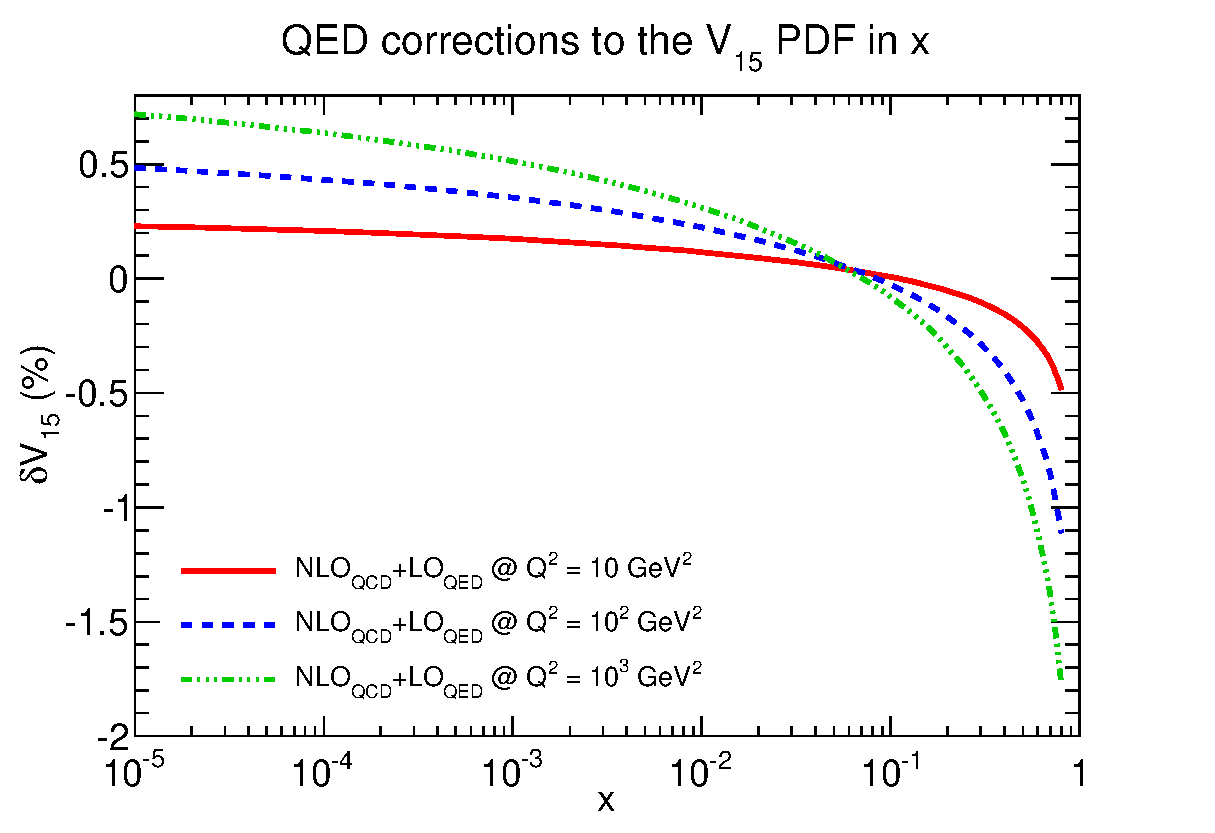
\includegraphics[scale=0.45]{plots/v15_glike}
\par\end{centering}

\begin{centering}
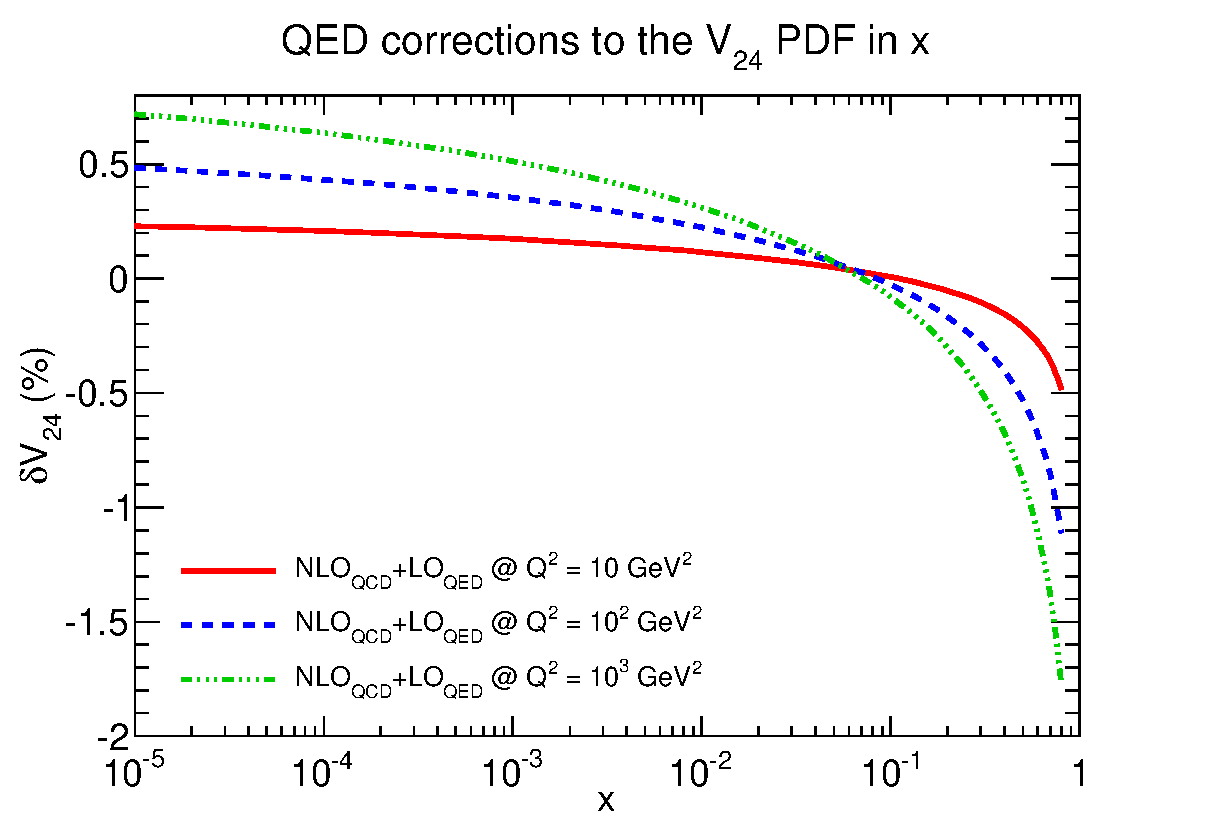
\includegraphics[scale=0.45]{plots/v24_glike}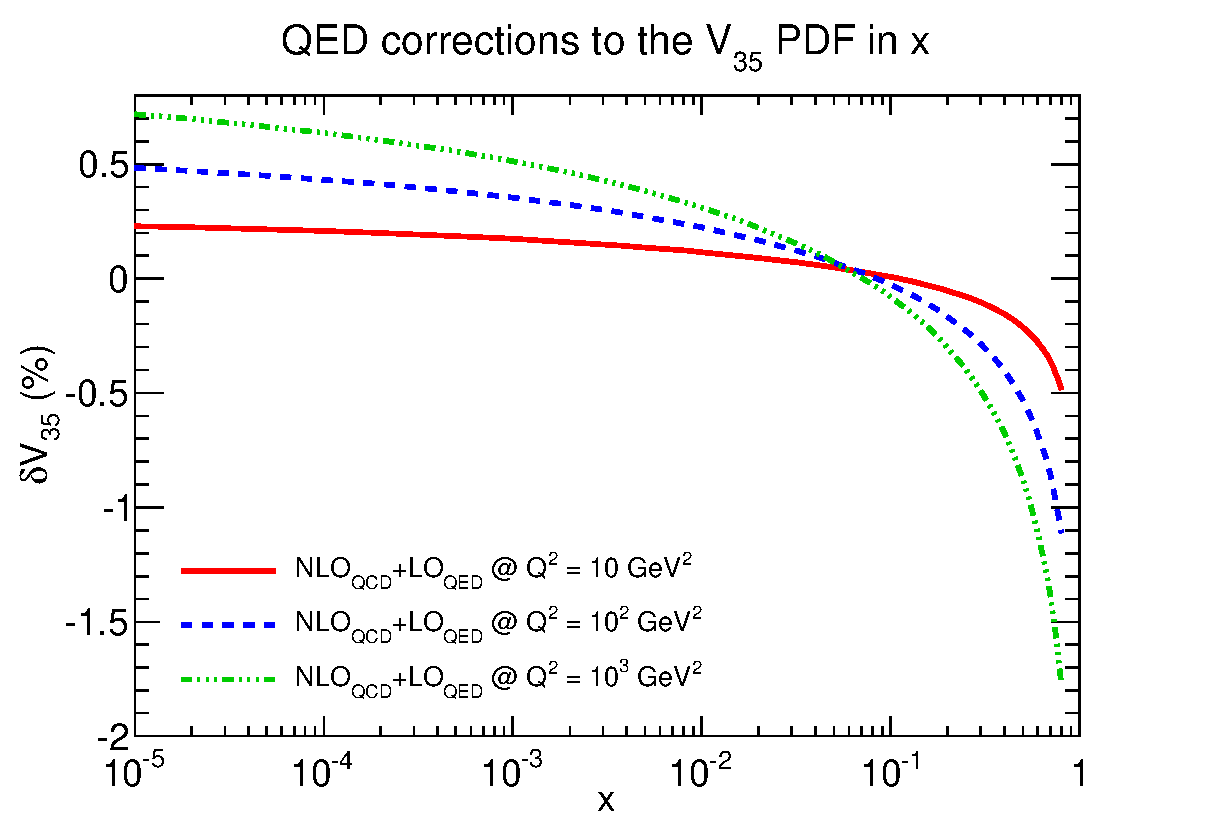
\includegraphics[scale=0.45]{plots/v35_glike}
\par\end{centering}

\caption{\label{fig:Impact-of-QED-figure-2a}Impact of QED correction for the
valence family. $x\gamma(x,Q_{0}^{2})=\alpha/\alpha_{S}xg(x,Q_{0}^{2})$}
\end{figure}


\begin{figure}
\begin{centering}
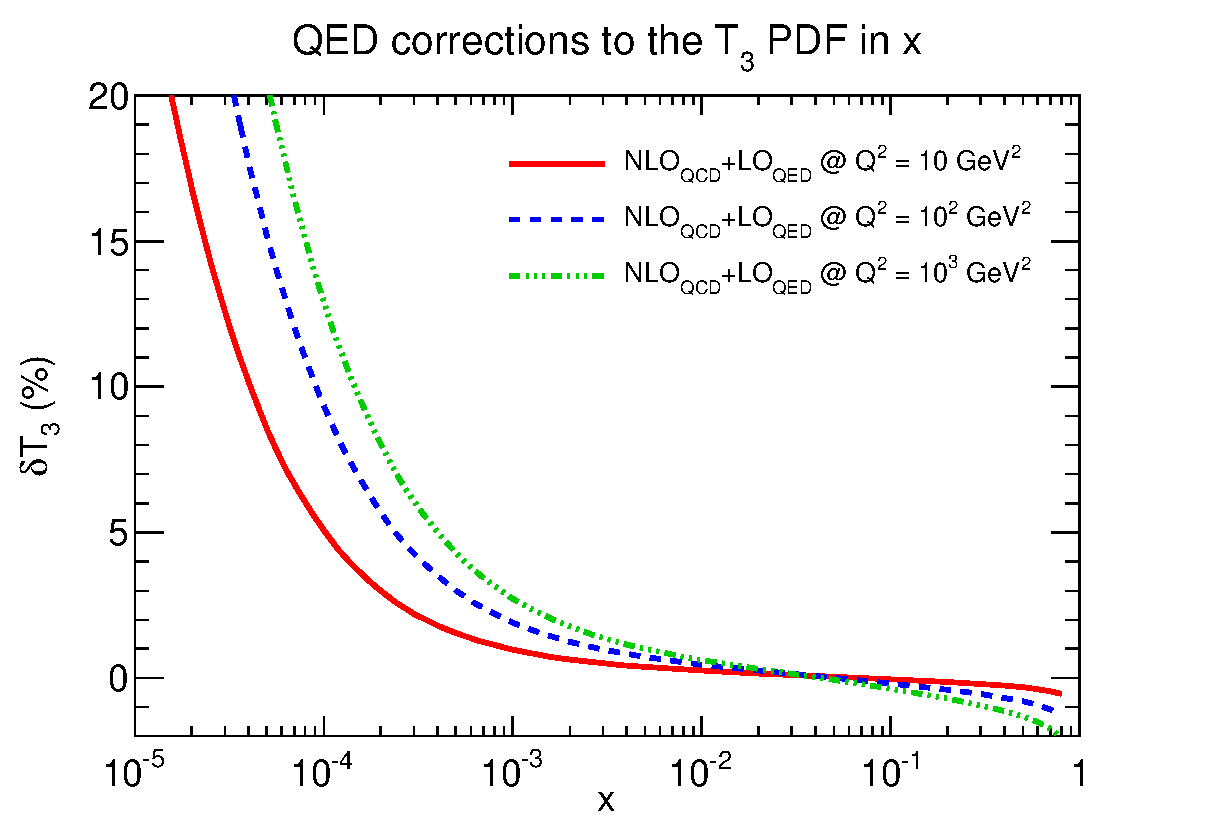
\includegraphics[scale=0.45]{plots/t03_glike}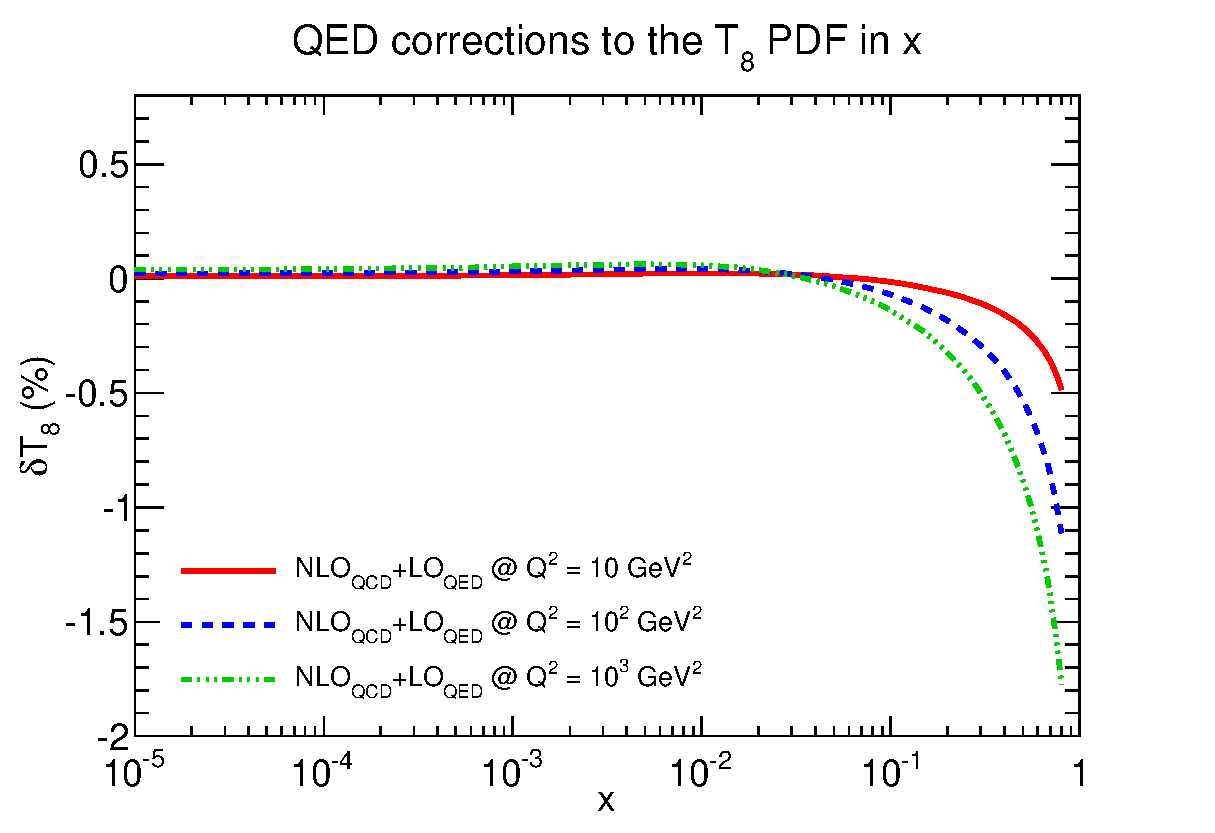
\includegraphics[scale=0.45]{plots/t08_glike}
\par\end{centering}

\begin{centering}
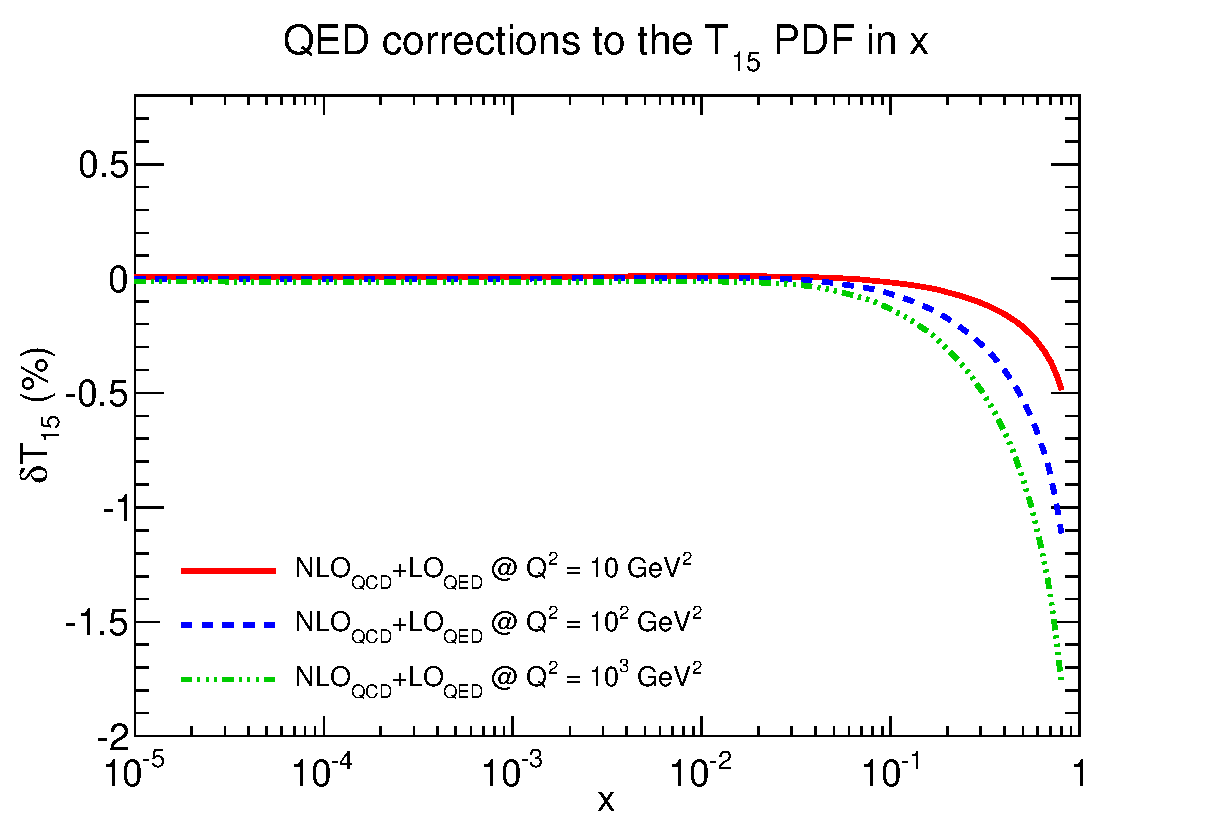
\includegraphics[scale=0.45]{plots/t15_glike}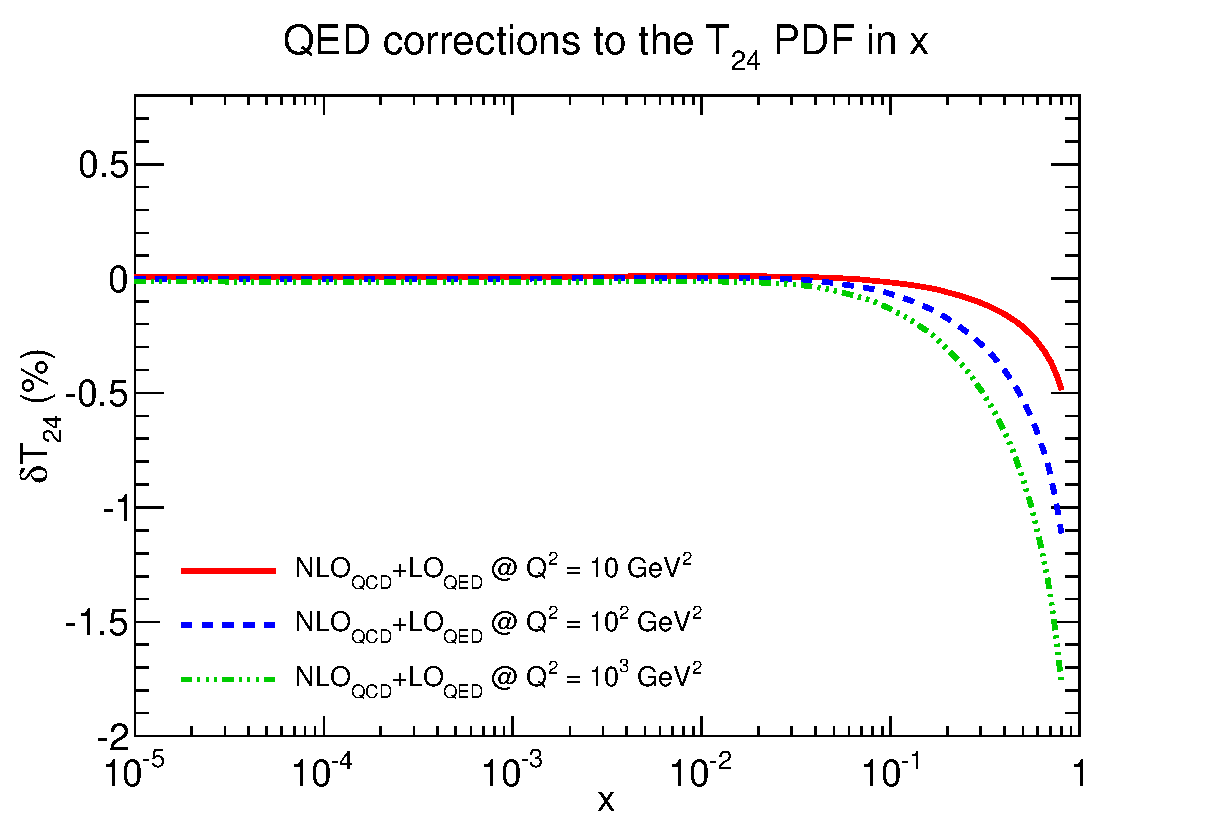
\includegraphics[scale=0.45]{plots/t24_glike}
\par\end{centering}

\begin{centering}
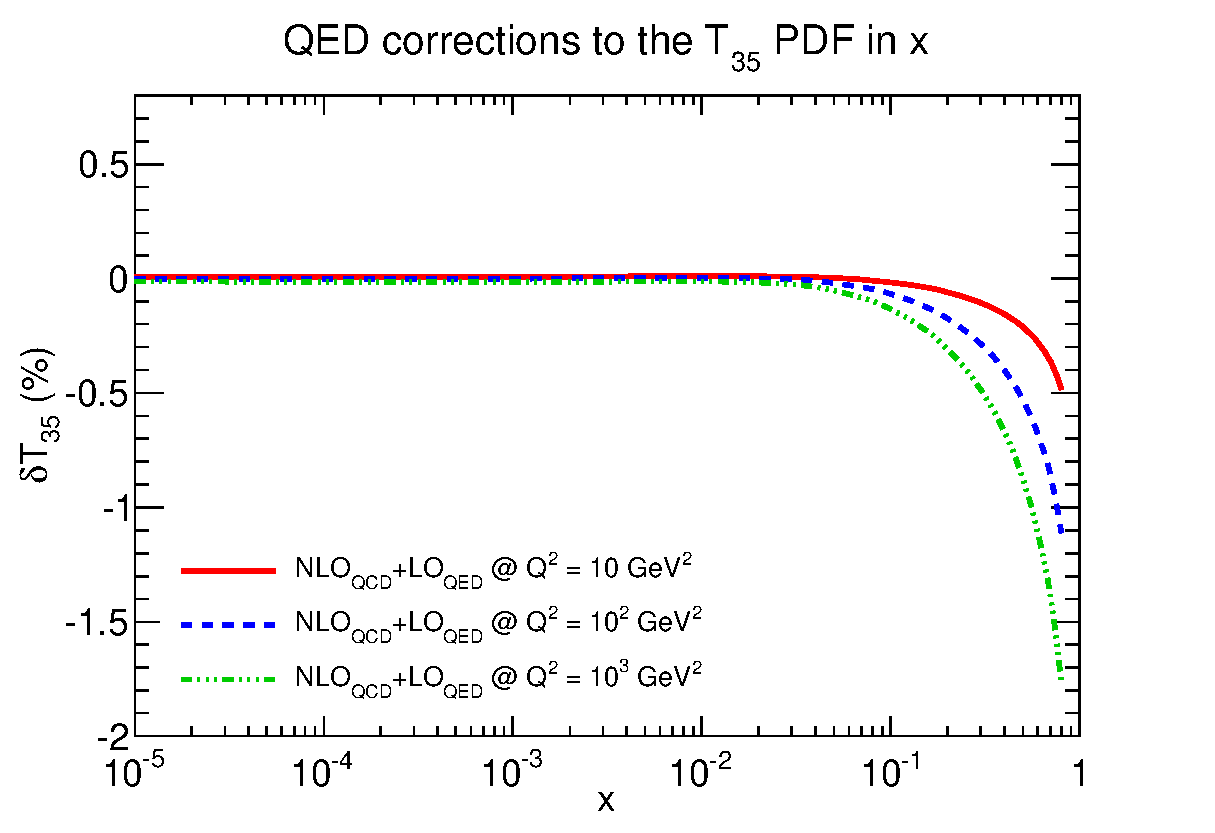
\includegraphics[scale=0.45]{plots/t35_glike}
\par\end{centering}

\caption{\label{fig:Impact-of-QED-figure-3a}Impact of QED correction for the
$T$ family. $x\gamma(x,Q_{0}^{2})=\alpha/\alpha_{S}xg(x,Q_{0}^{2})$}
\end{figure}


\begin{table}
\begin{centering}
\subfloat[From $Q_{0}^{2}=2\,\text{GeV}^{2}$ to $Q^{2}=10\,\text{GeV}^{2}$]{\begin{centering}
\begin{tabular}{|c|c|c|c|c|c|c|c|c|}
\hline 
$x$  & $10^{-5}$  & $10^{-4}$  & $10^{-3}$  & $10^{-2}$  & $10^{-1}$  & $0.3$  & $0.7$ & $0.8$\tabularnewline
\hline 
\hline 
$\delta g$ (\%)  &  &  &  &  &  &  &  & \tabularnewline
\hline 
$\delta\Sigma$ (\%)  &  &  &  &  &  &  &  & \tabularnewline
\hline 
$\delta u$ (\%)  &  &  &  &  &  &  &  & \tabularnewline
\hline 
$\delta d$ (\%)  &  &  &  &  &  &  &  & \tabularnewline
\hline 
$\delta s$ (\%)  &  &  &  &  &  &  &  & \tabularnewline
\hline 
$\delta V$ (\%)  &  &  &  &  &  &  &  & \tabularnewline
\hline 
$\delta V_{3}$ (\%)  &  &  &  &  &  &  &  & \tabularnewline
\hline 
$\delta V_{8}$ (\%)  &  &  &  &  &  &  &  & \tabularnewline
\hline 
$\delta V_{15}$ (\%)  &  &  &  &  &  &  &  & \tabularnewline
\hline 
$\delta T_{3}$ (\%)  &  &  &  &  &  &  &  & \tabularnewline
\hline 
$\delta T_{8}$ (\%)  &  &  &  &  &  &  &  & \tabularnewline
\hline 
$\delta T_{15}$ (\%)  &  &  &  &  &  &  &  & \tabularnewline
\hline 
\end{tabular}
\par\end{centering}

}
\par\end{centering}

\begin{centering}
\subfloat[From $Q_{0}^{2}=2\,\text{GeV}^{2}$ to $Q^{2}=100\,\text{GeV}^{2}$.]{\begin{centering}
\begin{tabular}{|c|c|c|c|c|c|c|c|c|}
\hline 
$x$  & $10^{-5}$  & $10^{-4}$  & $10^{-3}$  & $10^{-2}$  & $10^{-1}$  & $0.3$  & $0.7$ & $0.8$\tabularnewline
\hline 
\hline 
$\delta g$ (\%)  &  &  &  &  &  &  &  & \tabularnewline
\hline 
$\delta\Sigma$ (\%)  &  &  &  &  &  &  &  & \tabularnewline
\hline 
$\delta u$ (\%)  &  &  &  &  &  &  &  & \tabularnewline
\hline 
$\delta d$ (\%)  &  &  &  &  &  &  &  & \tabularnewline
\hline 
$\delta s$ (\%)  &  &  &  &  &  &  &  & \tabularnewline
\hline 
$\delta V$ (\%)  &  &  &  &  &  &  &  & \tabularnewline
\hline 
$\delta V_{3}$ (\%)  &  &  &  &  &  &  &  & \tabularnewline
\hline 
$\delta V_{8}$ (\%)  &  &  &  &  &  &  &  & \tabularnewline
\hline 
$\delta V_{15}$ (\%)  &  &  &  &  &  &  &  & \tabularnewline
\hline 
$\delta T_{3}$ (\%)  &  &  &  &  &  &  &  & \tabularnewline
\hline 
$\delta T_{8}$ (\%)  &  &  &  &  &  &  &  & \tabularnewline
\hline 
$\delta T_{15}$ (\%)  &  &  &  &  &  &  &  & \tabularnewline
\hline 
\end{tabular}
\par\end{centering}

}
\par\end{centering}

\begin{centering}
\subfloat[From $Q_{0}^{2}=2\,\text{GeV}^{2}$ to $Q^{2}=1000\,\text{GeV}^{2}$.]{\begin{centering}
\begin{tabular}{|c|c|c|c|c|c|c|c|c|}
\hline 
$x$  & $10^{-5}$  & $10^{-4}$  & $10^{-3}$  & $10^{-2}$  & $10^{-1}$  & $0.3$  & $0.7$ & $0.8$\tabularnewline
\hline 
\hline 
$\delta g$ (\%)  &  &  &  &  &  &  &  & \tabularnewline
\hline 
$\delta\Sigma$ (\%)  &  &  &  &  &  &  &  & \tabularnewline
\hline 
$\delta u$ (\%)  &  &  &  &  &  &  &  & \tabularnewline
\hline 
$\delta d$ (\%)  &  &  &  &  &  &  &  & \tabularnewline
\hline 
$\delta s$ (\%)  &  &  &  &  &  &  &  & \tabularnewline
\hline 
$\delta V$ (\%)  &  &  &  &  &  &  &  & \tabularnewline
\hline 
$\delta V_{3}$ (\%)  &  &  &  &  &  &  &  & \tabularnewline
\hline 
$\delta V_{8}$ (\%)  &  &  &  &  &  &  &  & \tabularnewline
\hline 
$\delta V_{15}$ (\%)  &  &  &  &  &  &  &  & \tabularnewline
\hline 
$\delta T_{3}$ (\%)  &  &  &  &  &  &  &  & \tabularnewline
\hline 
$\delta T_{8}$ (\%)  &  &  &  &  &  &  &  & \tabularnewline
\hline 
$\delta T_{15}$ (\%)  &  &  &  &  &  &  &  & \tabularnewline
\hline 
\end{tabular}
\par\end{centering}

}
\par\end{centering}

\caption{\label{tab:Relative-differences-table-2}Relative differences for
evolution with NLO QCD + LO QED. $x\gamma(x,Q_{0}^{2})=\alpha/\alpha_{S}xg(x,Q_{0}^{2})$}
\end{table}


\begin{figure}
\begin{centering}
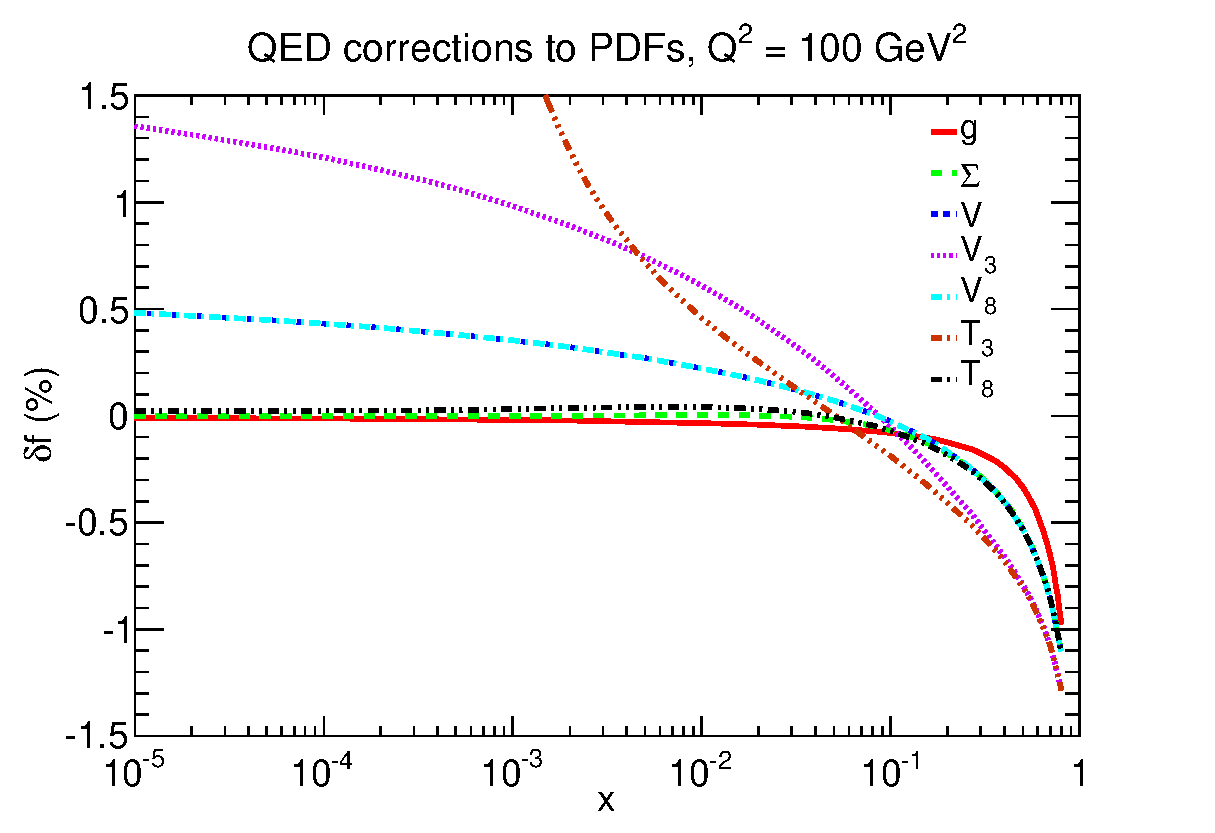
\includegraphics[scale=0.45]{plots/allPDFs_glike}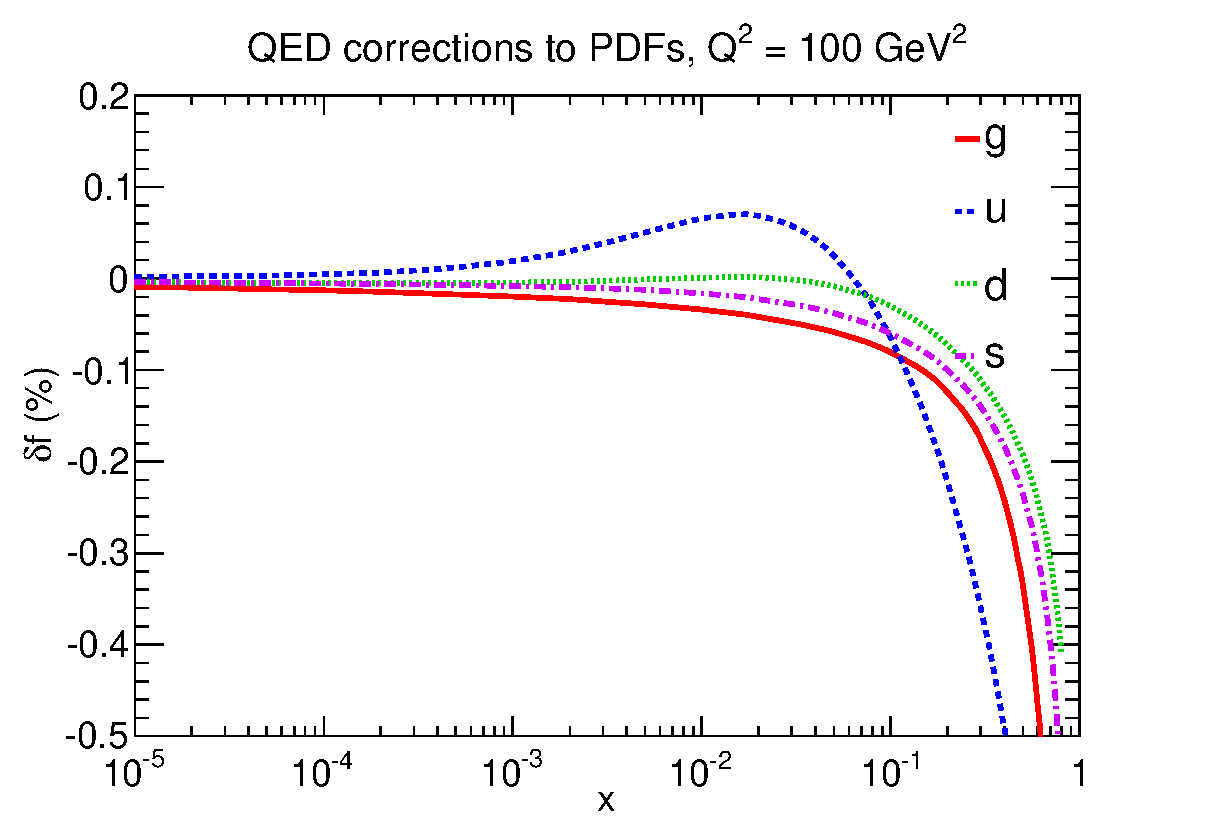
\includegraphics[scale=0.45]{plots/lhaPDFs_glike}
\par\end{centering}

\begin{centering}
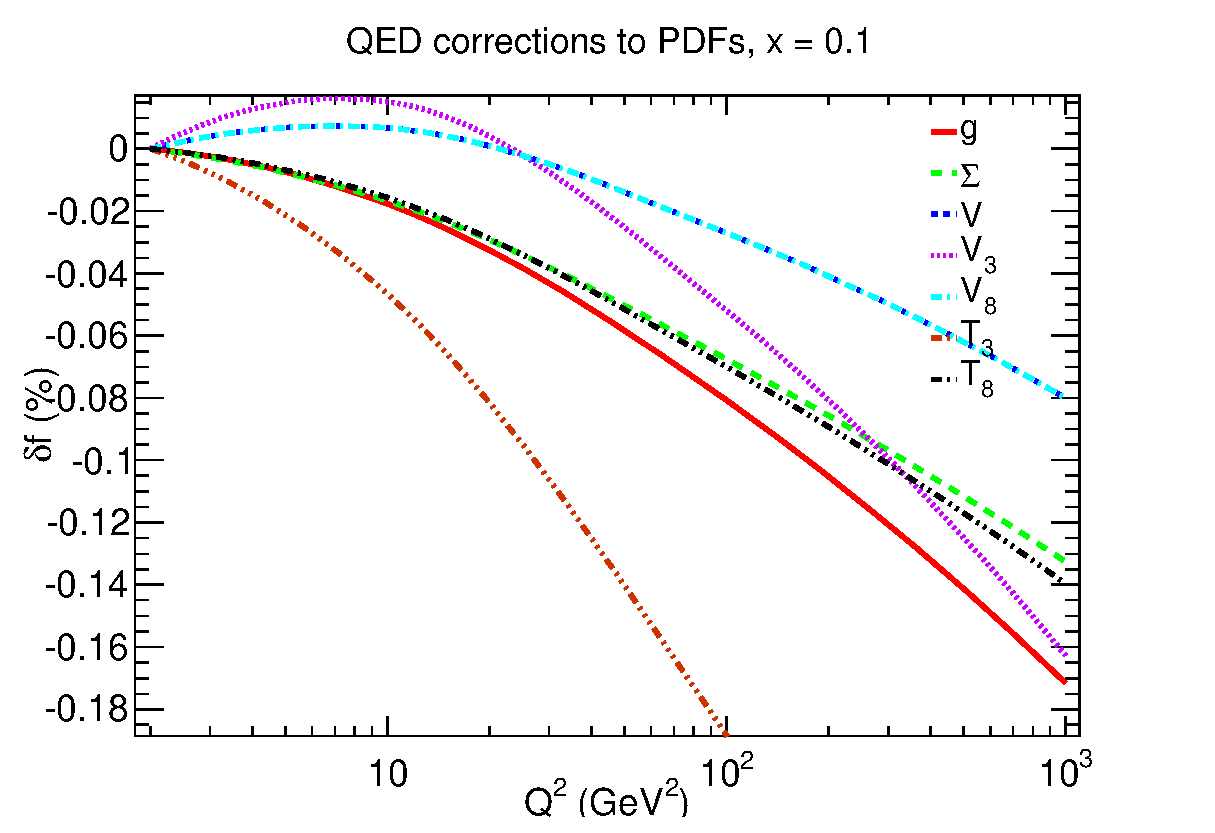
\includegraphics[scale=0.45]{plots/allPDFsQ_glike}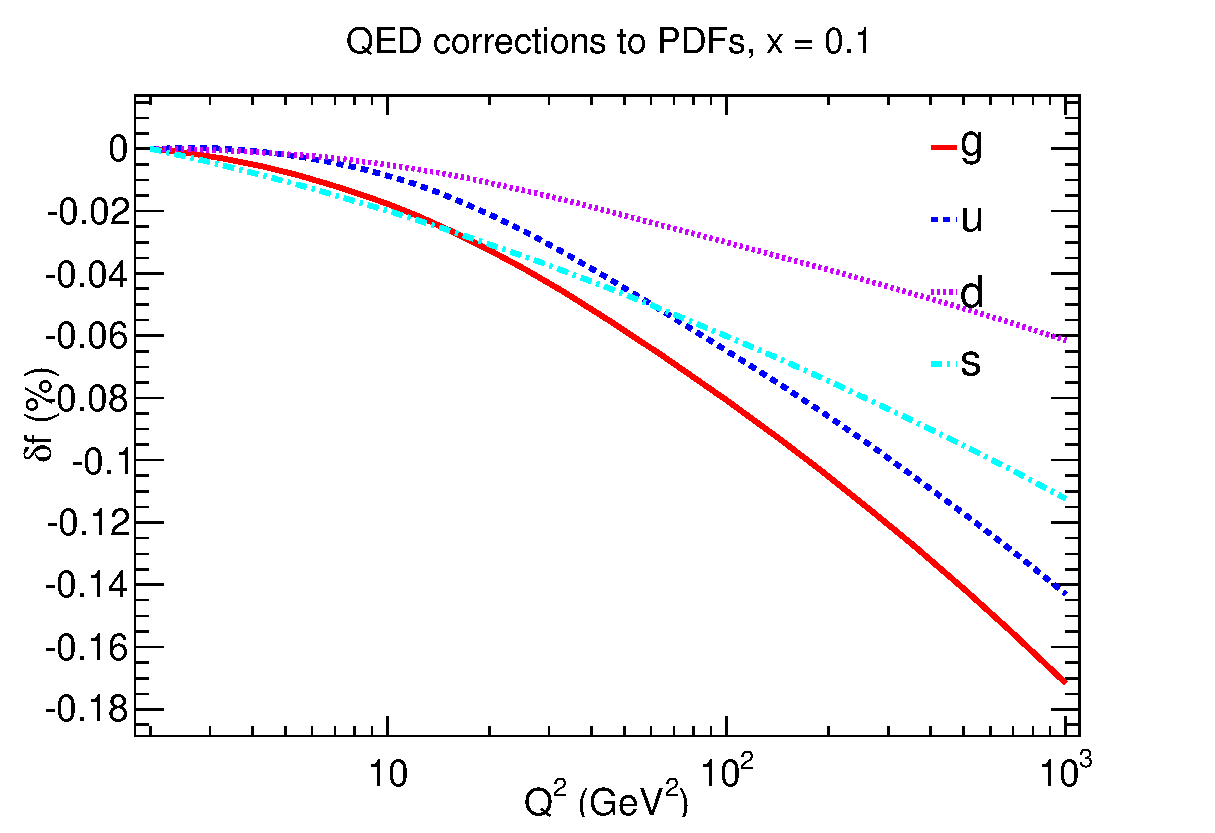
\includegraphics[scale=0.45]{plots/lhaPDFsQ_glike}
\par\end{centering}

\caption{\label{fig:Summary-with-all-1b}Summary with all PDFs together. $x\gamma(x,Q_{0}^{2})=\alpha/\alpha_{S}xg(x,Q_{0}^{2})$}
\end{figure}



\subsection{The $x\gamma(x,Q^{2})$ PDF in FFNS}

Figure \ref{fig:Photonpdf} shows the shape of the photon PDF obtained
dynamically. The left plot was obtained using the initial condition
$x\gamma(x,Q_{0}^{2})=0$, on the other hand the right plot was obtained
by imposing $x\gamma(x,Q_{0}^{2})\propto xg(x,Q_{0}^{2})$. From the
previous plots we observe that these prescriptions doesn't change
much the results.

\begin{figure}[H]
\begin{centering}
\subfloat[$x\gamma(x,Q_{0}^{2})=0$]{\begin{centering}
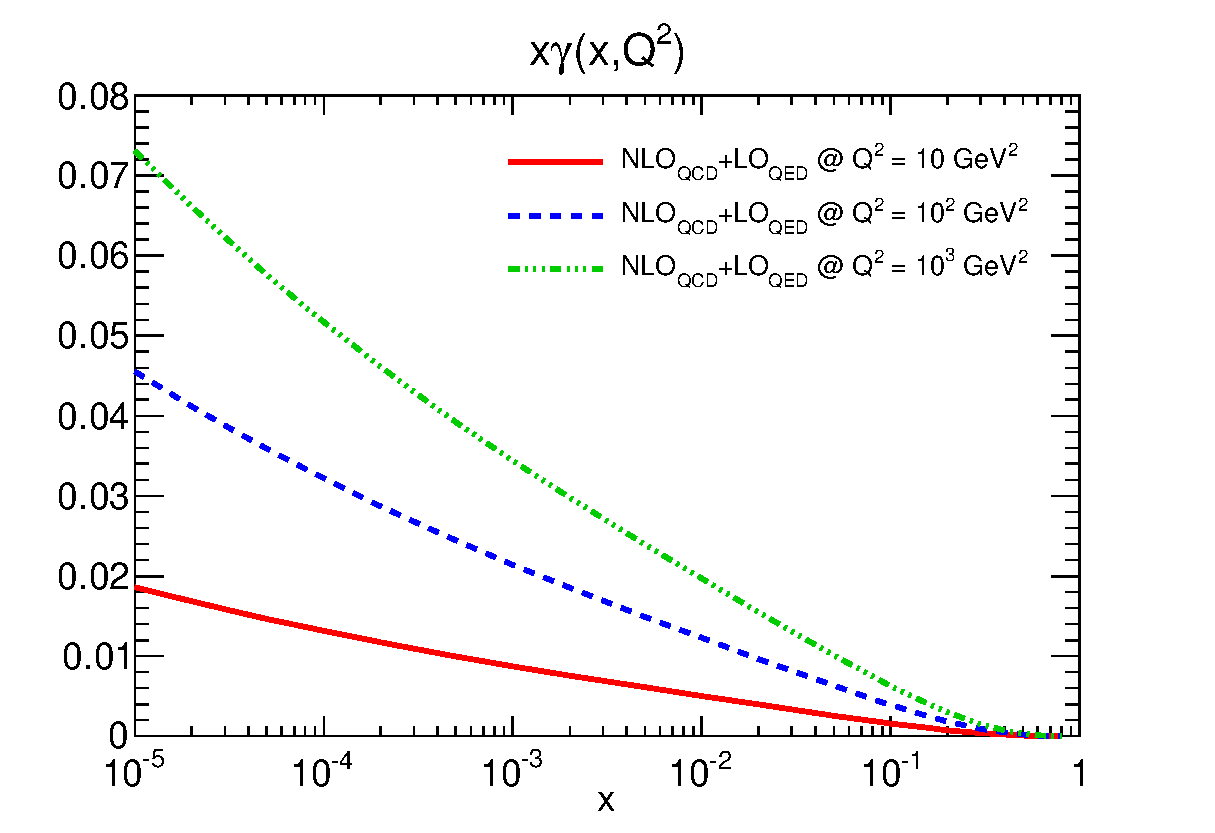
\includegraphics[scale=0.45]{plots/photon}
\par\end{centering}



}\subfloat[$x\gamma(x,Q_{0}^{2})=\alpha/\alpha_{S}xg(x,Q_{0}^{2})$]{\begin{centering}
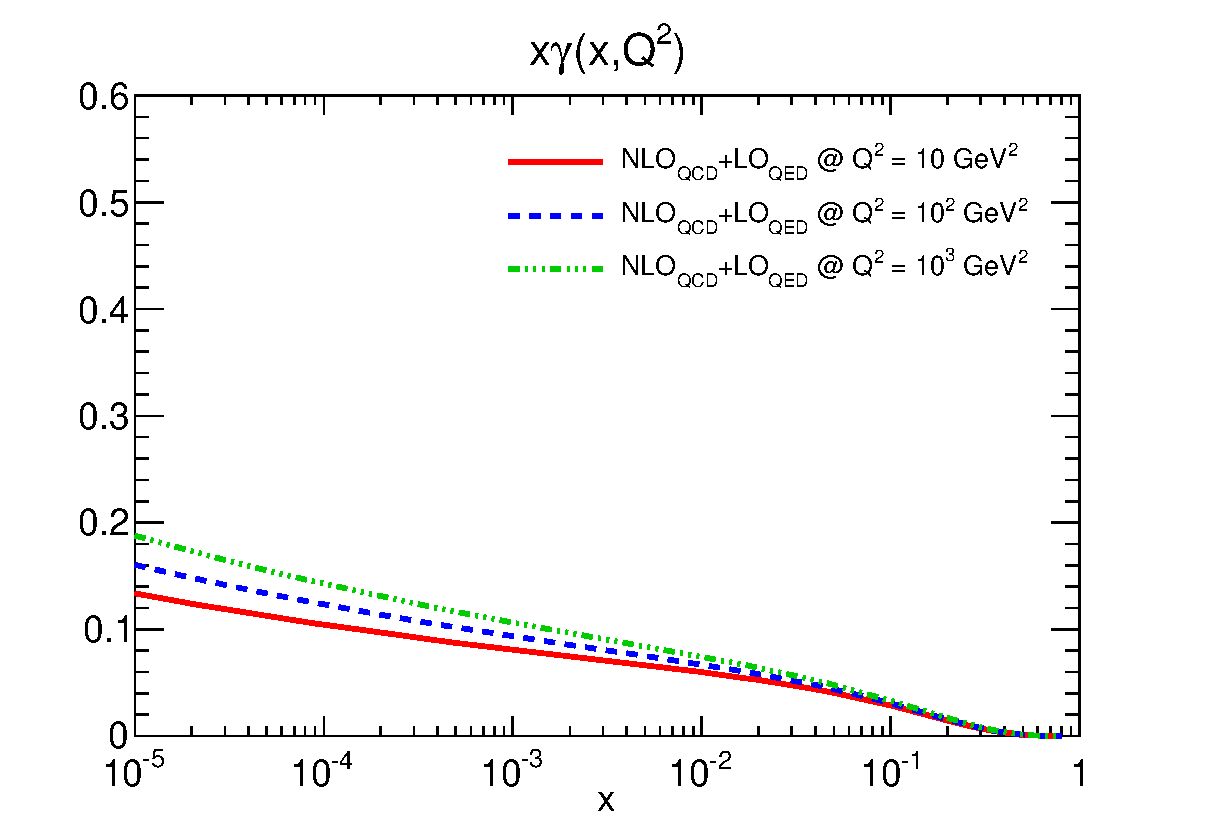
\includegraphics[scale=0.45]{plots/photon_glike}
\par\end{centering}

}
\par\end{centering}

\caption{\label{fig:Photonpdf}The PDF of the photon, multiplied by $x$, generated
by radiation.}
\end{figure}



\section{Implementation of the QED Corrections in the Variable Flavour Number
Scheme}

In this section we discuss the implementation of the of the QED correction
in the VFNS. Presently the code is actually able to perform both the
QCD and QED evolution in the VFNS separately but not at the same time.

As an example, what it does for the crossing of the charm threshold
is the following for the QCD evolution(%
\footnote{Here we are not cosidering the possibility af a discontinuos matching
at the heavy quark mass threshold as it happens for the NNLO evolution.%
}): 
\begin{equation}
\mathbf{f}^{(4,4)}(\mu^{2},\nu^{2})=\mathbf{G}^{(4)}(\mu^{2},m_{c}^{2})\cdot\mathbf{G}^{(3)}(m_{c}^{2},\mu_{0}^{2})\cdot\mathbf{f}^{(3,4)}(\mu_{0}^{2},\nu^{2})
\end{equation}
and the following for the QED evolution: 
\begin{equation}
\mathbf{f}^{(4,4)}(\mu^{2},\nu^{2})=\widetilde{\mathbf{G}}^{(4)}(\nu^{2},m_{c}^{2})\cdot\widetilde{\mathbf{G}}^{(3)}(m_{c}^{2},\nu_{0}^{2})\cdot\mathbf{f}^{(4,3)}(\mu^{2},\nu_{0}^{2})
\end{equation}
But to perform QCD and QED evolution at the same time, instead, one
should do the following: 
\begin{equation}
\mathbf{f}^{(4,4)}=\mathbf{G}^{(4)}\cdot\widetilde{\mathbf{G}}^{(4)}\cdot\mathbf{G}^{(3)}\cdot\widetilde{\mathbf{G}}^{(3)}\cdot\mathbf{f}^{(3,3)}\label{altogether}
\end{equation}


Notwithstanding, the code is only able to produce the quantities $\mathbf{G}^{(4)}\cdot\mathbf{G}^{(3)}$
and $\widetilde{\mathbf{G}}^{(4)}\cdot\widetilde{\mathbf{G}}^{(3)}$
separately. One may wonder then if it is possible to reconstruct eq.
(\ref{altogether}) starting from these two quantities. Unfortunately
the answer is not. But then one may ask what is the error the one
makes if considers the product $\mathbf{G}^{(4)}\cdot\mathbf{G}^{(3)}\cdot\widetilde{\mathbf{G}}^{(4)}\cdot\widetilde{\mathbf{G}}^{(3)}$.
Let's see: 
\begin{equation}
\mathbf{G}^{(4)}\cdot\widetilde{\mathbf{G}}^{(4)}\cdot\mathbf{G}^{(3)}\cdot\widetilde{\mathbf{G}}^{(3)}-\mathbf{G}^{(4)}\cdot\mathbf{G}^{(3)}\cdot\widetilde{\mathbf{G}}^{(4)}\cdot\widetilde{\mathbf{G}}^{(3)}=\mathbf{G}^{(4)}\cdot\left[\widetilde{\mathbf{G}}^{(4)},\mathbf{G}^{(3)}\right]\cdot\widetilde{\mathbf{G}}^{(3)}
\end{equation}
but since: 
\begin{equation}
\widetilde{\mathbf{G}}^{(4)}=\exp\left[\alpha\widetilde{\mathbf{A}}^{(4)}\right]\quad\mbox{and}\quad\mathbf{G}^{(3)}=\exp\left[\alpha_{s}\mathbf{A}^{(3)}\right]
\end{equation}
using the Baker-Campbell-Hausdorff formula one finds that: 
\begin{equation}
\left[\widetilde{\mathbf{G}}^{(4)},\mathbf{G}^{(3)}\right]=\alpha\alpha_{s}\left[\widetilde{\mathbf{A}}^{(4)},\mathbf{A}^{(3)}\right]+\mbox{higher order terms}
\end{equation}
therefore it is a subleading difference.

In the following sections we present the impact of QED+QCD evolution
versus QCD only evolution using \texttt{toyLH\_NLO.LHgrid} as input
PDF


\subsection{VNFS Initial condition $x\gamma(x,Q_{0}^{2})=0$}

Lets suppose that $x\gamma(x,Q_{0}^{2})=0$ at $Q_{0}^{2}=2\,\text{GeV}^{2}$,
the relative difference between PDFs evolved with NLO QCD and NLO
QCD + LO QED is showed in: Figure \ref{fig:Impact-of-QED-figure-1}
for the singlet sector, Figure \ref{fig:Impact-of-QED-figure-2-1}
for the valence, and Figure \ref{fig:Impact-of-QED-figure-3-1} for
the triplet.

We observe differences of 1\% at high $x$ for the singlet sector,
and in particular, the triplet is strongly modified at small-$x$.
This fact can be explained by the isospin symmetry breaking, in fact
$T_{3}$ highlights precisely the presence of different electric charges
for $up$ and $down$ partons.

Table \ref{tab:Relative-differences-table-1} illustrates for each
PDF flavour the relative difference at common values of $x$. Finally,
Figure \ref{fig:Summary-with-all-1} shows the comparison between
the relative difference of all PDFs and the $Q^{2}$ dependence of
the relative ratio.

\begin{figure}[H]
\begin{centering}
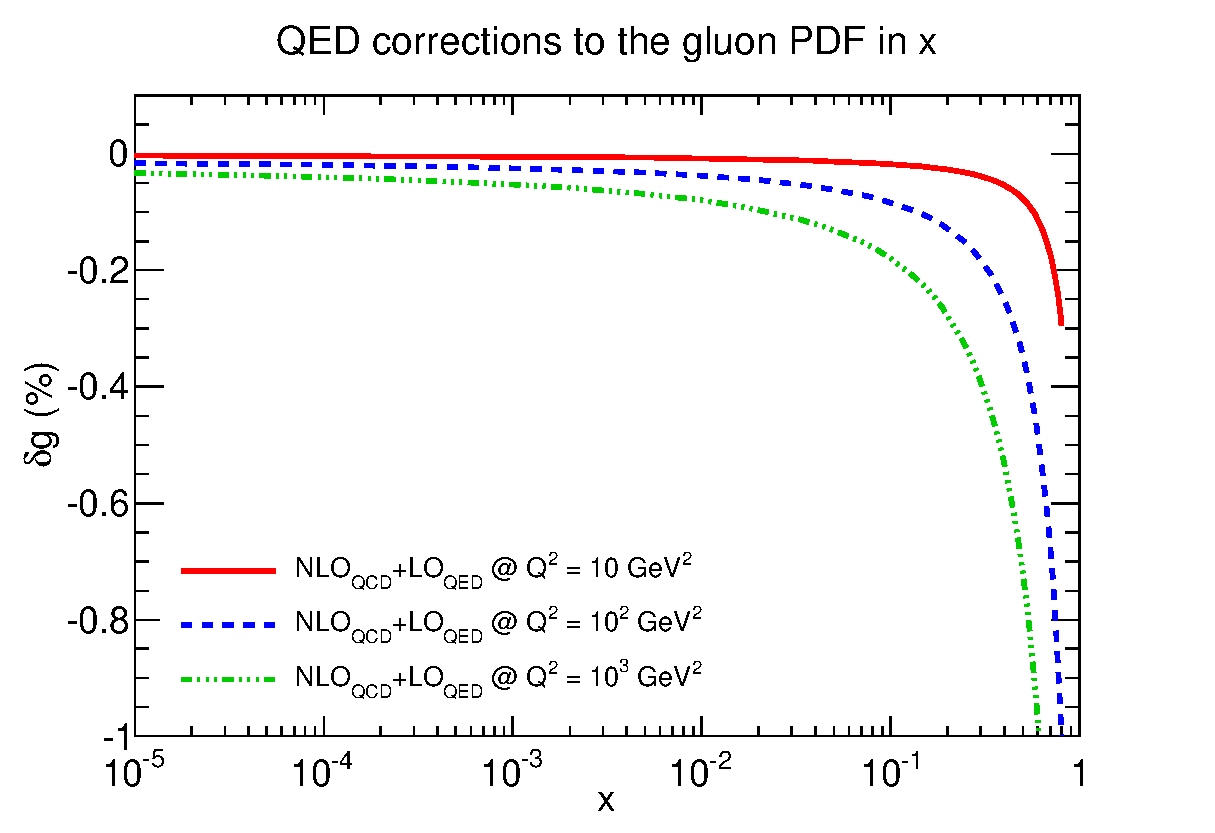
\includegraphics[scale=0.45]{plots/gluon_vnfs}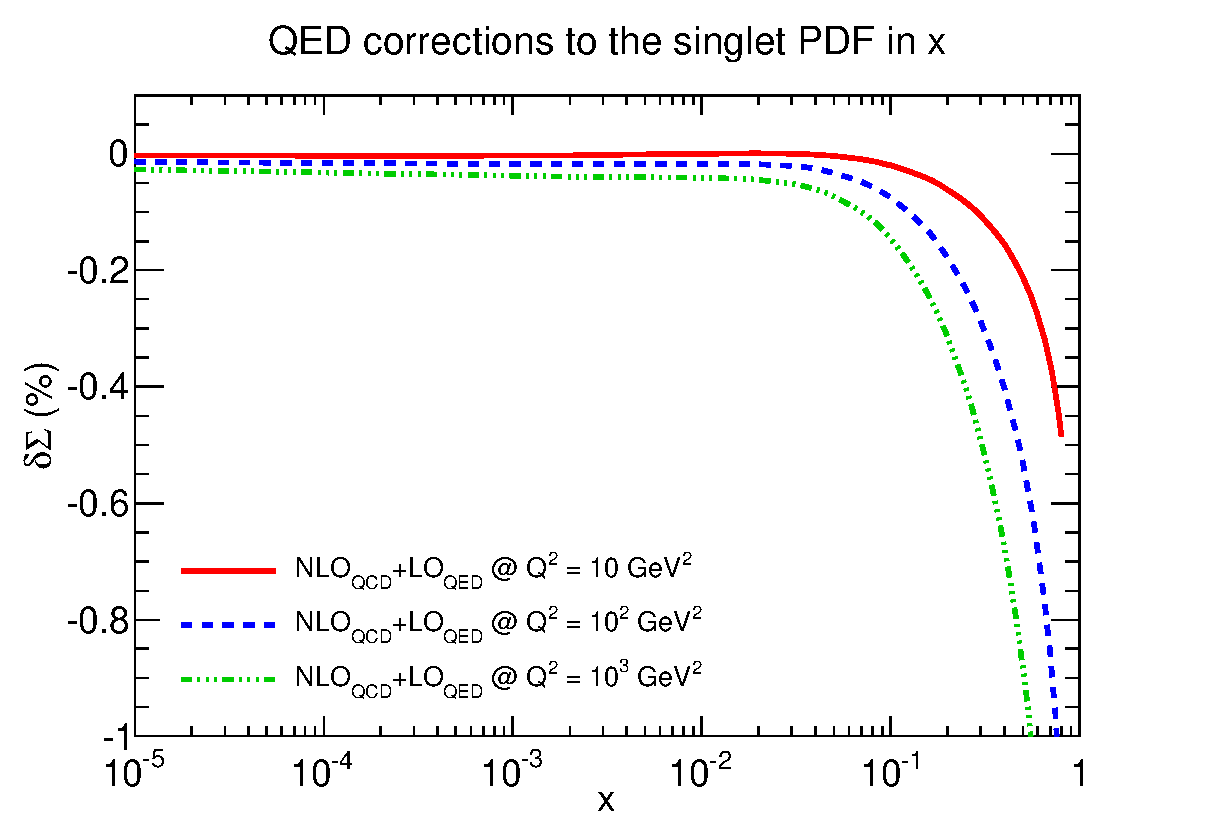
\includegraphics[scale=0.45]{plots/singlet_vnfs}
\par\end{centering}

\begin{centering}
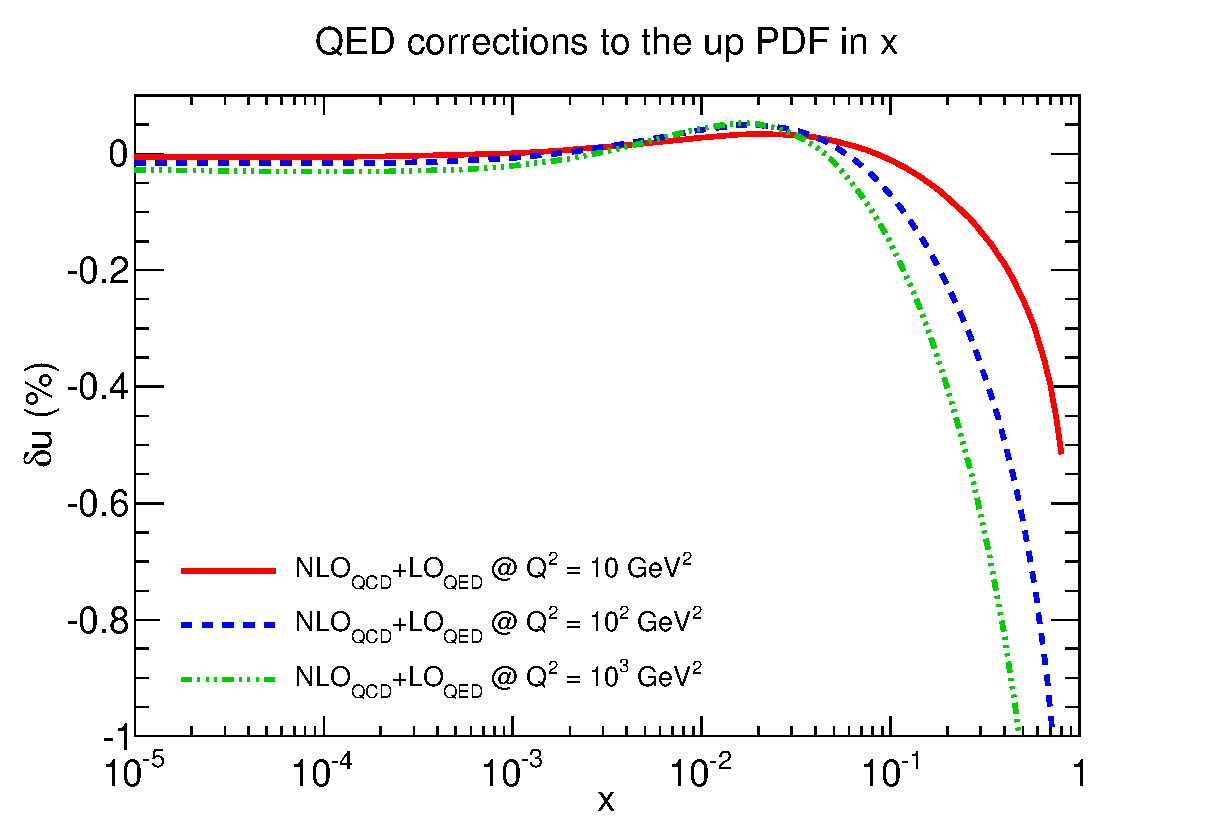
\includegraphics[scale=0.45]{plots/u_vnfs}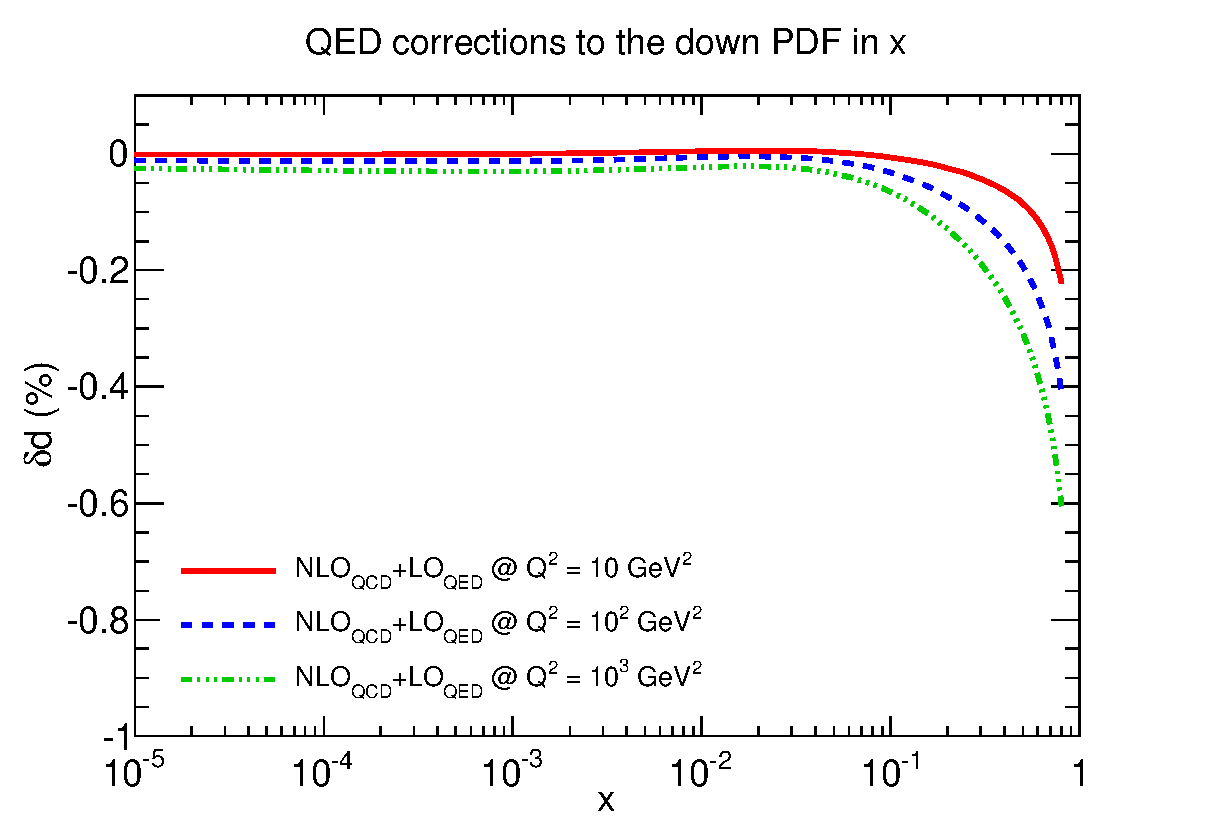
\includegraphics[scale=0.45]{plots/d_vnfs}
\par\end{centering}

\begin{centering}
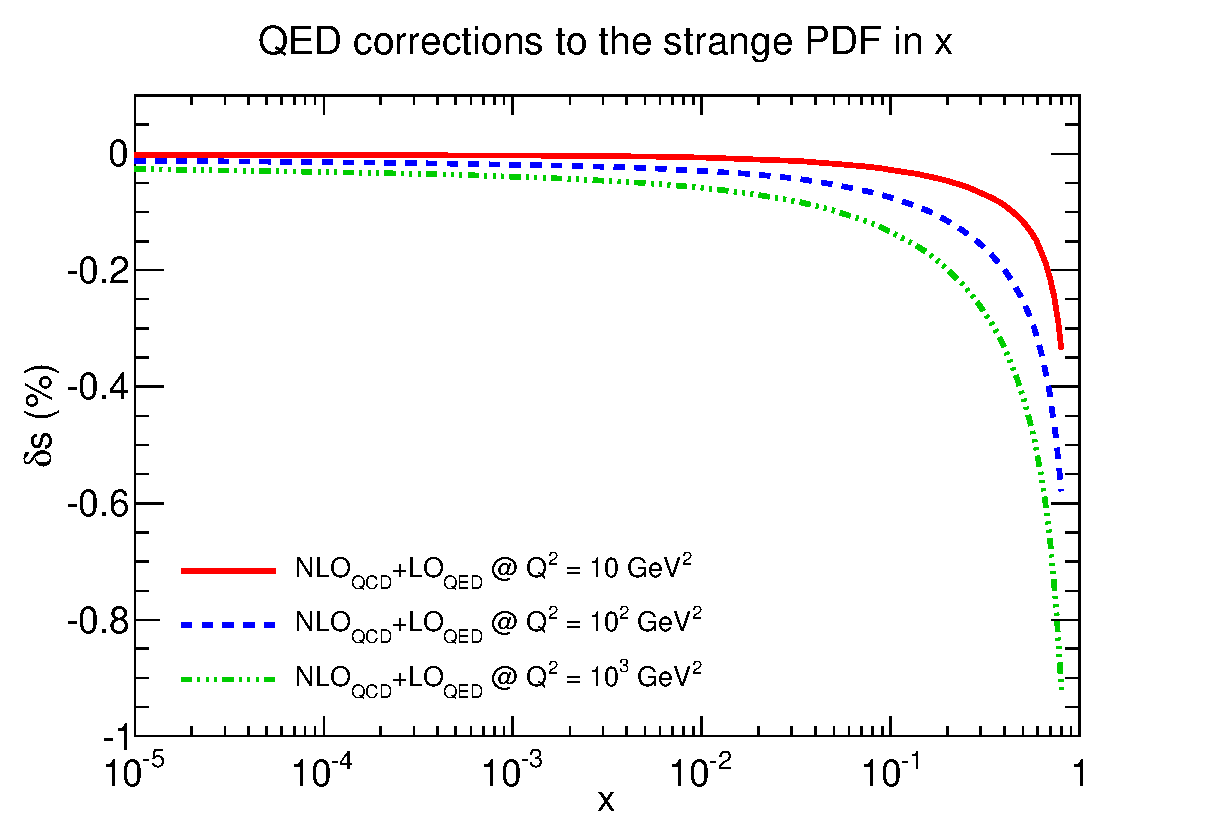
\includegraphics[scale=0.45]{plots/s_vnfs}
\par\end{centering}

\caption{\label{fig:Impact-of-QED-figure-1}Impact of QED correction for $g,u,d,s,\Sigma$
PDFs. $x\gamma(x,Q_{0}^{2})=0$.}
\end{figure}


\begin{figure}
\begin{centering}
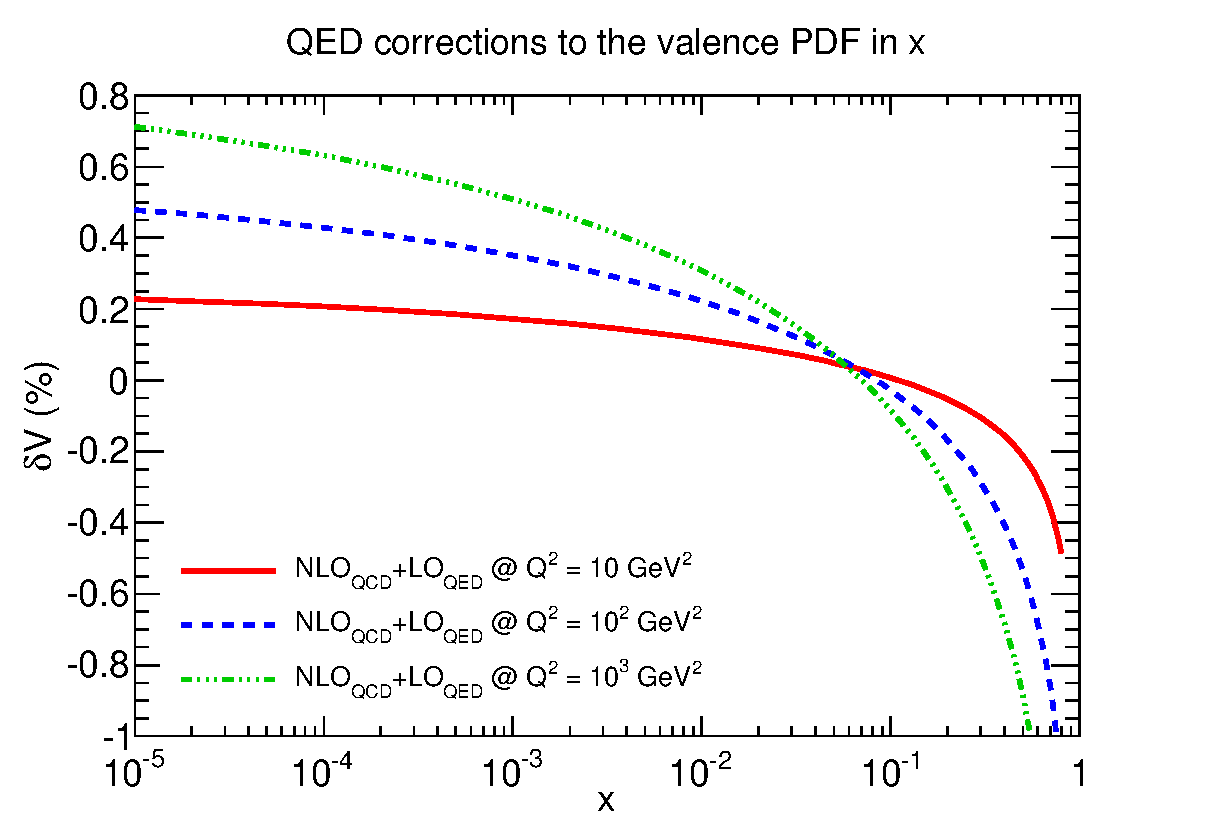
\includegraphics[scale=0.45]{plots/val_vnfs}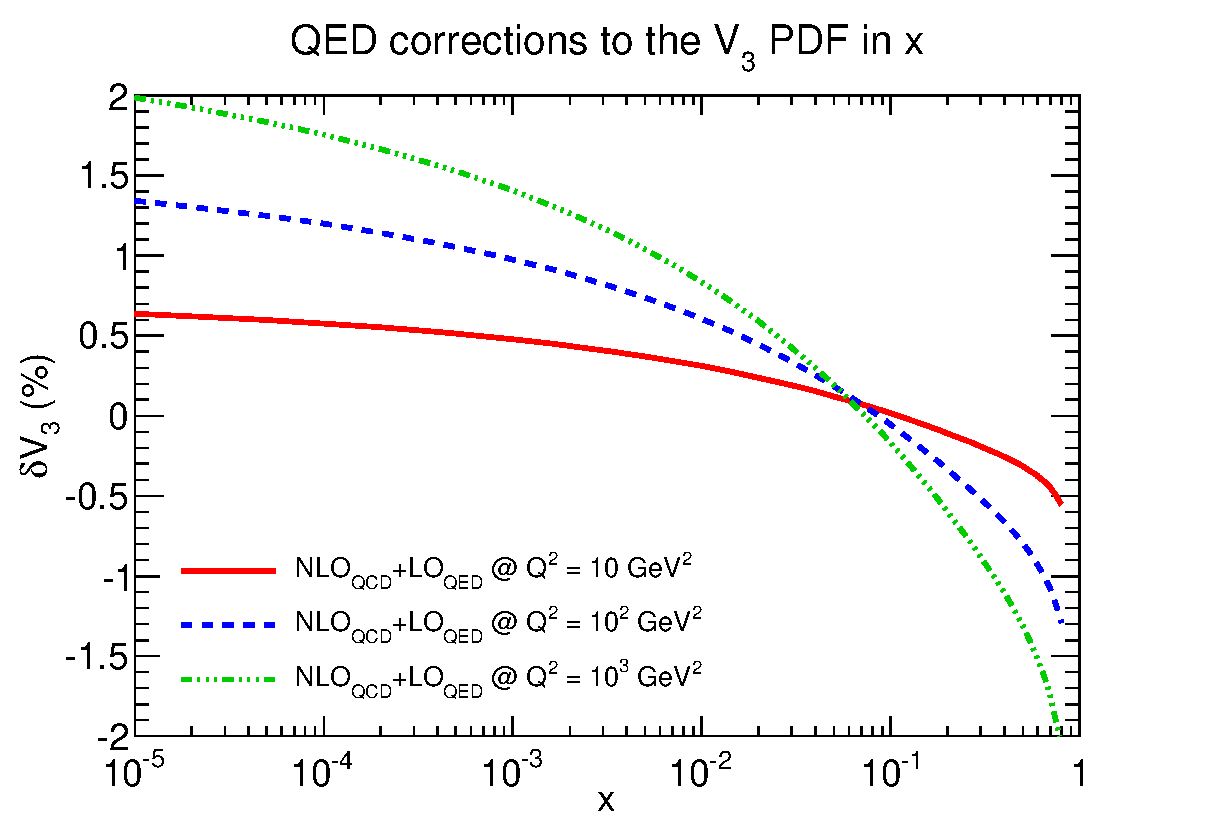
\includegraphics[scale=0.45]{plots/v03_vnfs}
\par\end{centering}

\begin{centering}
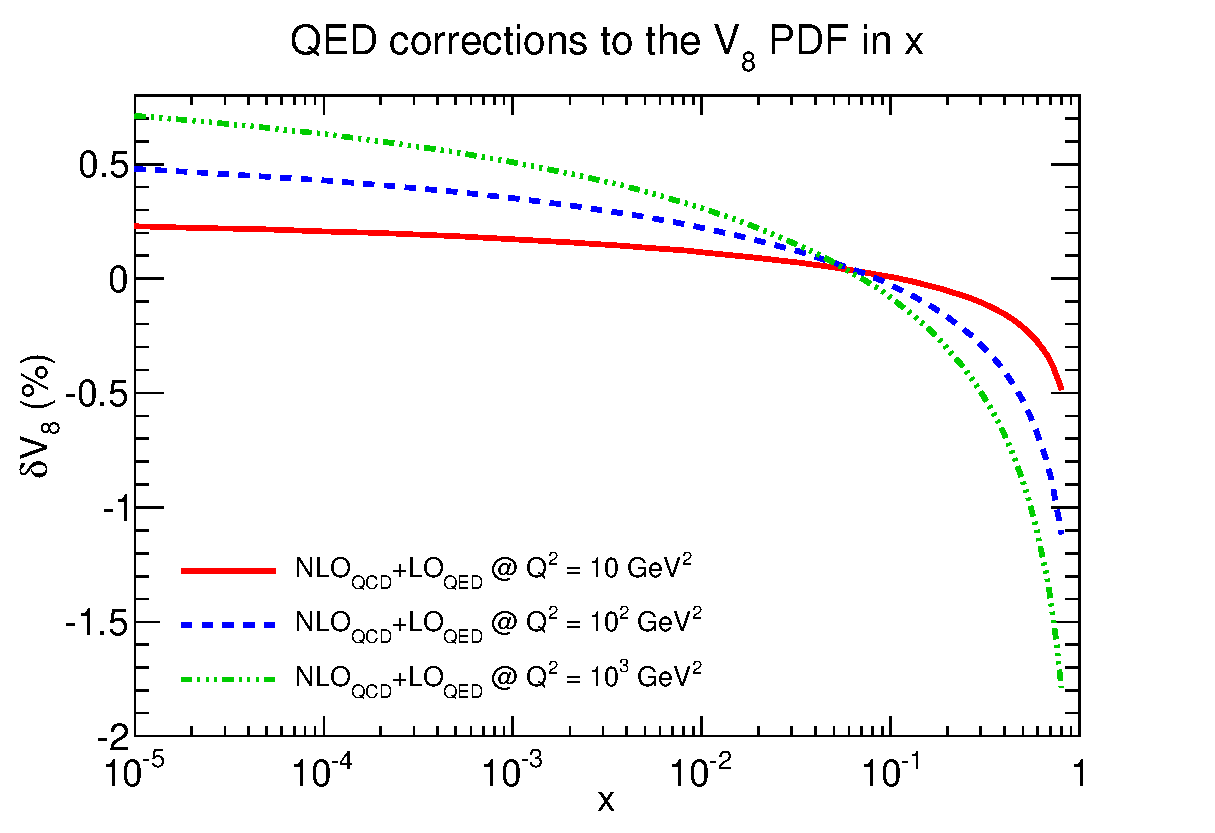
\includegraphics[scale=0.45]{plots/v08_vnfs}\includegraphics[scale=0.45]{plots/v15}
\par\end{centering}

\begin{centering}
\includegraphics[scale=0.45]{plots/v24_vnfs}\includegraphics[scale=0.45]{plots/v35_vnfs}
\par\end{centering}

\caption{\label{fig:Impact-of-QED-figure-2-1}Impact of QED correction for
the valence family. $x\gamma(x,Q_{0}^{2})=0$}
\end{figure}


\begin{figure}
\begin{centering}
\includegraphics[scale=0.45]{plots/t03_vnfs}\includegraphics[scale=0.45]{plots/t08_vnfs}
\par\end{centering}

\begin{centering}
\includegraphics[scale=0.45]{plots/t15_vnfs}\includegraphics[scale=0.45]{plots/t24_vnfs}
\par\end{centering}

\begin{centering}
\includegraphics[scale=0.45]{plots/t35_vnfs}
\par\end{centering}

\caption{\label{fig:Impact-of-QED-figure-3-1}Impact of QED correction for
the $T$ family. $x\gamma(x,Q_{0}^{2})=0$}
\end{figure}


\begin{table}
\begin{centering}
\subfloat[From $Q_{0}^{2}=2\,\text{GeV}^{2}$ to $Q^{2}=10\,\text{GeV}^{2}$]{\begin{centering}
\begin{tabular}{|c|c|c|c|c|c|c|c|c|}
\hline 
$x$  & $10^{-5}$  & $10^{-4}$  & $10^{-3}$  & $10^{-2}$  & $10^{-1}$  & $0.3$  & $0.7$ & $0.8$\tabularnewline
\hline 
\hline 
$\delta g$ (\%)  &  &  &  &  &  &  &  & \tabularnewline
\hline 
$\delta\Sigma$ (\%)  &  &  &  &  &  &  &  & \tabularnewline
\hline 
$\delta u$ (\%)  &  &  &  &  &  &  &  & \tabularnewline
\hline 
$\delta d$ (\%)  &  &  &  &  &  &  &  & \tabularnewline
\hline 
$\delta s$ (\%)  &  &  &  &  &  &  &  & \tabularnewline
\hline 
$\delta V$ (\%)  &  &  &  &  &  &  &  & \tabularnewline
\hline 
$\delta V_{3}$ (\%)  &  &  &  &  &  &  &  & \tabularnewline
\hline 
$\delta V_{8}$ (\%)  &  &  &  &  &  &  &  & \tabularnewline
\hline 
$\delta V_{15}$ (\%)  &  &  &  &  &  &  &  & \tabularnewline
\hline 
$\delta T_{3}$ (\%)  &  &  &  &  &  &  &  & \tabularnewline
\hline 
$\delta T_{8}$ (\%)  &  &  &  &  &  &  &  & \tabularnewline
\hline 
$\delta T_{15}$ (\%)  &  &  &  &  &  &  &  & \tabularnewline
\hline 
\end{tabular}
\par\end{centering}

}
\par\end{centering}

\begin{centering}
\subfloat[From $Q_{0}^{2}=2\,\text{GeV}^{2}$ to $Q^{2}=100\,\text{GeV}^{2}$.]{\begin{centering}
\begin{tabular}{|c|c|c|c|c|c|c|c|c|}
\hline 
$x$  & $10^{-5}$  & $10^{-4}$  & $10^{-3}$  & $10^{-2}$  & $10^{-1}$  & $0.3$  & $0.7$ & $0.8$\tabularnewline
\hline 
\hline 
$\delta g$ (\%)  &  &  &  &  &  &  &  & \tabularnewline
\hline 
$\delta\Sigma$ (\%)  &  &  &  &  &  &  &  & \tabularnewline
\hline 
$\delta u$ (\%)  &  &  &  &  &  &  &  & \tabularnewline
\hline 
$\delta d$ (\%)  &  &  &  &  &  &  &  & \tabularnewline
\hline 
$\delta s$ (\%)  &  &  &  &  &  &  &  & \tabularnewline
\hline 
$\delta V$ (\%)  &  &  &  &  &  &  &  & \tabularnewline
\hline 
$\delta V_{3}$ (\%)  &  &  &  &  &  &  &  & \tabularnewline
\hline 
$\delta V_{8}$ (\%)  &  &  &  &  &  &  &  & \tabularnewline
\hline 
$\delta V_{15}$ (\%)  &  &  &  &  &  &  &  & \tabularnewline
\hline 
$\delta T_{3}$ (\%)  &  &  &  &  &  &  &  & \tabularnewline
\hline 
$\delta T_{8}$ (\%)  &  &  &  &  &  &  &  & \tabularnewline
\hline 
$\delta T_{15}$ (\%)  &  &  &  &  &  &  &  & \tabularnewline
\hline 
\end{tabular}
\par\end{centering}

}
\par\end{centering}

\begin{centering}
\subfloat[From $Q_{0}^{2}=2\,\text{GeV}^{2}$ to $Q^{2}=1000\,\text{GeV}^{2}$.]{\begin{centering}
\begin{tabular}{|c|c|c|c|c|c|c|c|c|}
\hline 
$x$  & $10^{-5}$  & $10^{-4}$  & $10^{-3}$  & $10^{-2}$  & $10^{-1}$  & $0.3$  & $0.7$ & $0.8$\tabularnewline
\hline 
\hline 
$\delta g$ (\%)  &  &  &  &  &  &  &  & \tabularnewline
\hline 
$\delta\Sigma$ (\%)  &  &  &  &  &  &  &  & \tabularnewline
\hline 
$\delta u$ (\%)  &  &  &  &  &  &  &  & \tabularnewline
\hline 
$\delta d$ (\%)  &  &  &  &  &  &  &  & \tabularnewline
\hline 
$\delta s$ (\%)  &  &  &  &  &  &  &  & \tabularnewline
\hline 
$\delta V$ (\%)  &  &  &  &  &  &  &  & \tabularnewline
\hline 
$\delta V_{3}$ (\%)  &  &  &  &  &  &  &  & \tabularnewline
\hline 
$\delta V_{8}$ (\%)  &  &  &  &  &  &  &  & \tabularnewline
\hline 
$\delta V_{15}$ (\%)  &  &  &  &  &  &  &  & \tabularnewline
\hline 
$\delta T_{3}$ (\%)  &  &  &  &  &  &  &  & \tabularnewline
\hline 
$\delta T_{8}$ (\%)  &  &  &  &  &  &  &  & \tabularnewline
\hline 
$\delta T_{15}$ (\%)  &  &  &  &  &  &  &  & \tabularnewline
\hline 
\end{tabular}
\par\end{centering}

}
\par\end{centering}

\caption{\label{tab:Relative-differences-table-1}Relative differences for
evolution with NLO QCD + LO QED. $x\gamma(x,Q_{0}^{2})=0$}
\end{table}


\begin{figure}
\begin{centering}
\includegraphics[scale=0.45]{plots/allPDFs_vnfs}\includegraphics[scale=0.45]{plots/lhaPDFs_vnfs}
\par\end{centering}

\begin{centering}
\includegraphics[scale=0.45]{plots/allPDFsQ_vnfs}\includegraphics[scale=0.45]{plots/lhaPDFsQ_vnfs}
\par\end{centering}

\caption{\label{fig:Summary-with-all-1}Summary with all PDFs together. $x\gamma(x,Q_{0}^{2})=0$}
\end{figure}


\newpage{}


\subsection{VNFS Initial condition $x\gamma(x,Q_{0}^{2})\propto xg(x,Q_{0}^{2})$}

Lets suppose now that $x\gamma(x,Q_{0}^{2})=\alpha/\alpha_{S}xg(x,Q_{0}^{2})$
at $Q_{0}^{2}=2\,\text{GeV}^{2}$, the relative difference between
PDFs evolved with NLO QCD and NLO QCD + LO QED is showed in: Figure
\ref{fig:Impact-of-QED-figure-1b-1} for the singlet sector, Figure
\ref{fig:Impact-of-QED-figure-2a-1} for the valence, and Figure \ref{fig:Impact-of-QED-figure-3a-1}
for the triplet.

We still observing differences of 1\% at high $x$ for the singlet
sector, and again, the triplet at is strongly modified at small-$x$.

Table \ref{tab:Relative-differences-table-2-1} illustrates for each
PDF the relative difference for specific $x$ values. Finally, Figure
\ref{fig:Summary-with-all-1b-1} shows the comparison between the
relative difference of all PDFs and the $Q^{2}$ dependence of the
relative ratio.

\begin{figure}[H]
\begin{centering}
\includegraphics[scale=0.45]{plots/gluon_vnfs_glike}\includegraphics[scale=0.45]{plots/singlet_vnfs_glike}
\par\end{centering}

\begin{centering}
\includegraphics[scale=0.45]{plots/u_vnfs_glike}\includegraphics[scale=0.45]{plots/d_vnfs_glike}
\par\end{centering}

\begin{centering}
\includegraphics[scale=0.45]{plots/s_vnfs_glike}
\par\end{centering}

\caption{\label{fig:Impact-of-QED-figure-1b-1}Impact of QED correction for
$g,u,d,s,\Sigma$ PDFs. $x\gamma(x,Q_{0}^{2})=\alpha/\alpha_{S}xg(x,Q_{0}^{2})$}
\end{figure}


\begin{figure}
\begin{centering}
\includegraphics[scale=0.45]{plots/val_vnfs_glike}\includegraphics[scale=0.45]{plots/v03_vnfs_glike}
\par\end{centering}

\begin{centering}
\includegraphics[scale=0.45]{plots/v08_vnfs_glike}\includegraphics[scale=0.45]{plots/v15_vnfs_glike}
\par\end{centering}

\begin{centering}
\includegraphics[scale=0.45]{plots/v24_vnfs_glike}\includegraphics[scale=0.45]{plots/v35_vnfs_glike}
\par\end{centering}

\caption{\label{fig:Impact-of-QED-figure-2a-1}Impact of QED correction for
the valence family. $x\gamma(x,Q_{0}^{2})=\alpha/\alpha_{S}xg(x,Q_{0}^{2})$}
\end{figure}


\begin{figure}
\begin{centering}
\includegraphics[scale=0.45]{plots/t03_vnfs_glike}\includegraphics[scale=0.45]{plots/t08_vnfs_glike}
\par\end{centering}

\begin{centering}
\includegraphics[scale=0.45]{plots/t15_vnfs_glike}\includegraphics[scale=0.45]{plots/t24_vnfs_glike}
\par\end{centering}

\begin{centering}
\includegraphics[scale=0.45]{plots/t35_vnfs_glike}
\par\end{centering}

\caption{\label{fig:Impact-of-QED-figure-3a-1}Impact of QED correction for
the $T$ family. $x\gamma(x,Q_{0}^{2})=\alpha/\alpha_{S}xg(x,Q_{0}^{2})$}
\end{figure}


\begin{table}
\begin{centering}
\subfloat[From $Q_{0}^{2}=2\,\text{GeV}^{2}$ to $Q^{2}=10\,\text{GeV}^{2}$]{\begin{centering}
\begin{tabular}{|c|c|c|c|c|c|c|c|c|}
\hline 
$x$  & $10^{-5}$  & $10^{-4}$  & $10^{-3}$  & $10^{-2}$  & $10^{-1}$  & $0.3$  & $0.7$ & $0.8$\tabularnewline
\hline 
\hline 
$\delta g$ (\%)  &  &  &  &  &  &  &  & \tabularnewline
\hline 
$\delta\Sigma$ (\%)  &  &  &  &  &  &  &  & \tabularnewline
\hline 
$\delta u$ (\%)  &  &  &  &  &  &  &  & \tabularnewline
\hline 
$\delta d$ (\%)  &  &  &  &  &  &  &  & \tabularnewline
\hline 
$\delta s$ (\%)  &  &  &  &  &  &  &  & \tabularnewline
\hline 
$\delta V$ (\%)  &  &  &  &  &  &  &  & \tabularnewline
\hline 
$\delta V_{3}$ (\%)  &  &  &  &  &  &  &  & \tabularnewline
\hline 
$\delta V_{8}$ (\%)  &  &  &  &  &  &  &  & \tabularnewline
\hline 
$\delta V_{15}$ (\%)  &  &  &  &  &  &  &  & \tabularnewline
\hline 
$\delta T_{3}$ (\%)  &  &  &  &  &  &  &  & \tabularnewline
\hline 
$\delta T_{8}$ (\%)  &  &  &  &  &  &  &  & \tabularnewline
\hline 
$\delta T_{15}$ (\%)  &  &  &  &  &  &  &  & \tabularnewline
\hline 
\end{tabular}
\par\end{centering}

}
\par\end{centering}

\begin{centering}
\subfloat[From $Q_{0}^{2}=2\,\text{GeV}^{2}$ to $Q^{2}=100\,\text{GeV}^{2}$.]{\begin{centering}
\begin{tabular}{|c|c|c|c|c|c|c|c|c|}
\hline 
$x$  & $10^{-5}$  & $10^{-4}$  & $10^{-3}$  & $10^{-2}$  & $10^{-1}$  & $0.3$  & $0.7$ & $0.8$\tabularnewline
\hline 
\hline 
$\delta g$ (\%)  &  &  &  &  &  &  &  & \tabularnewline
\hline 
$\delta\Sigma$ (\%)  &  &  &  &  &  &  &  & \tabularnewline
\hline 
$\delta u$ (\%)  &  &  &  &  &  &  &  & \tabularnewline
\hline 
$\delta d$ (\%)  &  &  &  &  &  &  &  & \tabularnewline
\hline 
$\delta s$ (\%)  &  &  &  &  &  &  &  & \tabularnewline
\hline 
$\delta V$ (\%)  &  &  &  &  &  &  &  & \tabularnewline
\hline 
$\delta V_{3}$ (\%)  &  &  &  &  &  &  &  & \tabularnewline
\hline 
$\delta V_{8}$ (\%)  &  &  &  &  &  &  &  & \tabularnewline
\hline 
$\delta V_{15}$ (\%)  &  &  &  &  &  &  &  & \tabularnewline
\hline 
$\delta T_{3}$ (\%)  &  &  &  &  &  &  &  & \tabularnewline
\hline 
$\delta T_{8}$ (\%)  &  &  &  &  &  &  &  & \tabularnewline
\hline 
$\delta T_{15}$ (\%)  &  &  &  &  &  &  &  & \tabularnewline
\hline 
\end{tabular}
\par\end{centering}

}
\par\end{centering}

\begin{centering}
\subfloat[From $Q_{0}^{2}=2\,\text{GeV}^{2}$ to $Q^{2}=1000\,\text{GeV}^{2}$.]{\begin{centering}
\begin{tabular}{|c|c|c|c|c|c|c|c|c|}
\hline 
$x$  & $10^{-5}$  & $10^{-4}$  & $10^{-3}$  & $10^{-2}$  & $10^{-1}$  & $0.3$  & $0.7$ & $0.8$\tabularnewline
\hline 
\hline 
$\delta g$ (\%)  &  &  &  &  &  &  &  & \tabularnewline
\hline 
$\delta\Sigma$ (\%)  &  &  &  &  &  &  &  & \tabularnewline
\hline 
$\delta u$ (\%)  &  &  &  &  &  &  &  & \tabularnewline
\hline 
$\delta d$ (\%)  &  &  &  &  &  &  &  & \tabularnewline
\hline 
$\delta s$ (\%)  &  &  &  &  &  &  &  & \tabularnewline
\hline 
$\delta V$ (\%)  &  &  &  &  &  &  &  & \tabularnewline
\hline 
$\delta V_{3}$ (\%)  &  &  &  &  &  &  &  & \tabularnewline
\hline 
$\delta V_{8}$ (\%)  &  &  &  &  &  &  &  & \tabularnewline
\hline 
$\delta V_{15}$ (\%)  &  &  &  &  &  &  &  & \tabularnewline
\hline 
$\delta T_{3}$ (\%)  &  &  &  &  &  &  &  & \tabularnewline
\hline 
$\delta T_{8}$ (\%)  &  &  &  &  &  &  &  & \tabularnewline
\hline 
$\delta T_{15}$ (\%)  &  &  &  &  &  &  &  & \tabularnewline
\hline 
\end{tabular}
\par\end{centering}

}
\par\end{centering}

\caption{\label{tab:Relative-differences-table-2-1}Relative differences for
evolution with NLO QCD + LO QED. $x\gamma(x,Q_{0}^{2})=\alpha/\alpha_{S}xg(x,Q_{0}^{2})$}
\end{table}


\begin{figure}
\begin{centering}
\includegraphics[scale=0.45]{plots/allPDFs_vnfs_glike}\includegraphics[scale=0.45]{plots/lhaPDFs_vnfs_glike}
\par\end{centering}

\begin{centering}
\includegraphics[scale=0.45]{plots/allPDFsQ_vnfs_glike}\includegraphics[scale=0.45]{plots/lhaPDFsQ_vnfs_glike}
\par\end{centering}

\caption{\label{fig:Summary-with-all-1b-1}Summary with all PDFs together.
$x\gamma(x,Q_{0}^{2})=\alpha/\alpha_{S}xg(x,Q_{0}^{2})$}
\end{figure}



\subsection{The $x\gamma(x,Q^{2})$ PDF in VNFS}

Figure \ref{fig:Photonpdf-1} shows the shape of the photon PDF obtained
dynamically. The left plot was obtained using the initial condition
$x\gamma(x,Q_{0}^{2})=0$, on the other hand the right plot was obtained
by imposing $x\gamma(x,Q_{0}^{2})\propto xg(x,Q_{0}^{2})$. From the
previous plots we observe that these prescriptions doesn't change
much the results.

\begin{figure}[H]
\begin{centering}
\subfloat[$x\gamma(x,Q_{0}^{2})=0$]{\begin{centering}
\includegraphics[scale=0.45]{plots/photon_vnfs}
\par\end{centering}

}\subfloat[$x\gamma(x,Q_{0}^{2})=\alpha/\alpha_{S}xg(x,Q_{0}^{2})$]{\begin{centering}
\includegraphics[scale=0.45]{plots/photon_vnfs_glike}
\par\end{centering}

}
\par\end{centering}

\caption{\label{fig:Photonpdf-1}The PDF of the photon, multiplied by $x$,
generated by radiation.}
\end{figure}


\newpage{}


\section{Comparing results with Wienzierl code}

The only public available code of QCD+QED evolution is from \cite{Weinzierl},
we have used version 1.1.3 for the current benchmark, using our toyLH
as input PDF.


\subsection{Pure QCD comparison}

We have setup a $n_{f}=3$ system using our toyLH as input. Figure
\eqref{fig:Singlet-and-non-singlet} shows the results, the differences
achieve a maximum of 5\% for $x=[10^{-5},1]$. Which are due to different
algorithms and parametrization of the solution. We are showing the
best results we are able to produce with Weinzierl code.

\begin{figure}[H]
\begin{centering}
\includegraphics[scale=0.45]{plots/uvalence_wein}\includegraphics[scale=0.45]{plots/uvalence_wein_reldiff}
\par\end{centering}

\begin{centering}
\includegraphics[scale=0.45]{plots/g_wein}\includegraphics[scale=0.45]{plots/gluon_wein_reldiff}
\par\end{centering}

\begin{centering}
\includegraphics[scale=0.45]{plots/sigma_wein}\includegraphics[scale=0.45]{plots/sigma_wein_reldiff}
\par\end{centering}

\caption{Singlet and non-singlet sectors.\label{fig:Singlet-and-non-singlet}}


\end{figure}



\subsection{QCD+QED FFN comparison}

At this point we tried to compute the relative difference of PDFs
using Weinzierl code, fixing the photon PDF to zero at the initial
scale and using the FFN with $n_{f}=3$. Figure \eqref{fig:Comparison-between-Weinzierl}
presents the comparison between both predictions algorithms. We observe
that we have almost a good agreement between the singlet and valence
distributions, however we observe differences for the gluon PDF. The
origin of the discrepancies are possibly due to different algorithm
parametrization, i.e. integration accuracy, beta function definition.
For the gluon PDF the discrepancies are due to the different manipulation
of $\mathcal{O}(\alpha\alpha_{S})$ terms in both codes, and because
the relative differences are too small.

\begin{figure}[H]
\begin{centering}
\includegraphics[scale=0.45]{plots/u_wein}\includegraphics[scale=0.45]{plots/singlet_wein}
\par\end{centering}

\begin{centering}
\includegraphics[scale=0.45]{plots/gluon_wein}
\par\end{centering}

\caption{Comparison between Weinzierl code and our code.\label{fig:Comparison-between-Weinzierl}}


\end{figure}



\section{Benchmarking the algorithm}

Figure (\ref{fig:QED-coupling}) shows the $\alpha$ in function of
$Q^{2}$, highlighting the slope between different $n_{f}$ values.
Our evolution code uses the reference value $\alpha(m_{\tau}^{2})=7.496252\cdot10^{-3}$,
and performs the matching of $n_{f}$ automatically when $Q^{2}$
overtakes the quarks masses thresholds.

\begin{figure}[H]
\begin{centering}
\includegraphics[scale=0.4]{plots/alpharunning} 
\par\end{centering}

\caption{\label{fig:QED-coupling}QED coupling in function of the energy scale
$Q^{2}$: in our code the definition of $\alpha(Q^{2})$ is automatically
modified when energy thresholds are overtaking.}
\end{figure}


Figure (\ref{fig:Performance-results}) presents some code benchmark.
On the left the computational time is calculated for three algorithm:
path-ordering, numerical diagonalization, exponential expansion, the
difference between path-ordering and diagonalization is insignificant
for our scope so we implemented as the default algorithm the path-ordering
with 50 integration steps and exponential truncation at the 10th element.
The choise of these parameters can be illustrated by the right picture
of Figure (\ref{fig:Performance-results}), where we compute the relative
difference between path-ordering and diagonalization methods for the
Singlet $\Gamma_{\Sigma\Sigma}$ element, varying the parameters of
path-ordering.

\begin{figure}[H]
\begin{centering}
\includegraphics[scale=0.4]{plots/speed}\includegraphics[scale=0.4]{plots/precision} 
\par\end{centering}

\caption{\label{fig:Performance-results}Performance results when computing
the solution of QED evolution in $N$-space. On the left: time consumption
for three different algorithms. On the right: study of the solution
precision varying the path-ordering parameters.}
\end{figure}



\part{Building FastKernel tables}


\section{DIS observables}


\subsection{Structure functions $F_{2}^{\gamma,p}$ family}

For simplicity lets define our $F_{2}^{\gamma,p}$ as:
\begin{equation}
F_{2}^{\gamma,p}=a_{g}g+a_{\Sigma}\Sigma+a_{T_{3}}T_{3}+\frac{a_{T_{3}}}{3}T_{8}+a_{T_{15}}T_{15}+a_{T_{24}}T_{24}+a_{T_{35}}T_{35}
\end{equation}
with $a_{i}$ the DIS coefficient functions. Using pure QCD evolution
we obtain
\begin{equation}
\begin{cases}
g & =\Gamma_{gg}g_{0}+\Gamma_{gq}\Sigma_{0}\\
\Sigma & =\Gamma_{qg}g_{0}+\Gamma_{qq}\Sigma_{0}
\end{cases}\qquad\begin{cases}
T_{3} & =\Gamma^{+}T_{3,0}\\
T_{8} & =\Gamma^{+}T_{8,0}
\end{cases}
\end{equation}
\begin{equation}
\begin{cases}
T_{15} & =\Gamma_{15,g}g_{0}+\Gamma_{15,q}\Sigma_{0}\\
T_{24} & =\Gamma_{24,g}g_{0}+\Gamma_{24,q}\Sigma_{0}\\
T_{35} & =\Gamma_{35,g}g_{0}+\Gamma_{35,q}\Sigma_{0}
\end{cases}
\end{equation}
replacing this expression in the previous equation we get
\begin{align}
F_{2}^{\gamma,p} & =g_{0}\left(a_{g}\Gamma_{gg}+a_{\Sigma}\Gamma_{qg}+a_{T_{15}}\Gamma_{15,g}+a_{T_{24}}\Gamma_{24,g}+a_{T_{35}}\Gamma_{35,g}\right)\\
 & +\Sigma_{0}\left(a_{g}\Gamma_{gq}+a_{\Sigma}\Gamma_{qq}+a_{T_{15}}\Gamma_{15,q}+a_{T_{24}}\Gamma_{24,q}+a_{T_{35}}\Gamma_{35,q}\right)+a_{T_{3}}\Gamma^{+}\left(T_{3,0}+\frac{1}{3}T_{8,0}\right)
\end{align}


At this point lets introduce the QED evolution, by rewriting the evolution
equations using the 
\begin{equation}
\bm{\Gamma}_{QCD}\cdot(\mathbf{T}\cdot\bm{\Gamma}_{QED}\cdot\mathbf{T}^{-1})
\end{equation}
 product presented in the previous sections with $Q_{0}^{2}<m_{c}^{2}$
and $Q_{max}^{2}<m_{b}^{2}$, e.g. for the gluon we have:
\begin{equation}
g=\Gamma_{gg}g_{0}+\Gamma_{gq}\Gamma_{\Sigma\Sigma}\Sigma_{0}+\Gamma_{gq}\Gamma_{\Sigma\gamma}\gamma_{0}+\frac{1}{3}\Gamma_{gq}\Gamma_{\Sigma D}T_{8,0}-\frac{1}{3}\Gamma_{gq}\Gamma_{\Sigma D}T_{15,0}+\frac{1}{5}\Gamma_{gq}\Gamma_{\Sigma D}T_{24,0}-\frac{1}{5}\Gamma_{gq}\Gamma_{\Sigma D}T_{35,0}
\end{equation}


The only difference between this result and the previous one is the
presence of the $\gamma_{0}$ contributions. In order to simplify
the problem lets call 
\begin{equation}
a_{i,j}=\left(\Gamma_{\text{QCD}}^{\text{DIS}}\Gamma_{\text{QED}}\right)_{i,j}
\end{equation}
where $\Gamma_{\text{QCD}}^{\text{DIS}}$ are the QCD evolution kernels
multiplied by the relevant coefficient functions (SIGMADIS), then
the $F_{2}^{\gamma,p}$ can be written as (SIGMA\_QCED=$a_{i,j}$)
\begin{align}
F_{2}^{\gamma,p} & =\Sigma_{0}\left(a_{1,1}+a_{2,1}+a_{10,1}+\frac{a_{11,1}}{3}+a_{12,1}+a_{13,1}+a_{14,1}\right)\\
+ & g_{0}\left(a_{1,2}+a_{2,2}+a_{10,2}+\frac{a_{11,2}}{3}+a_{12,2}+a_{13,2}+a_{14,2}\right)\\
{\color{blue}+} & {\color{blue}\gamma_{0}\left(a_{1,3}+a_{2,3}+a_{10,3}+\frac{a_{11,3}}{3}+a_{12,3}+a_{13,3}+a_{14,3}\right)}\\
+ & T_{3,0}\left(a_{1,10}+a_{2,10}+a_{10,10}+\frac{a_{11,10}}{3}+a_{12,10}+a_{13,10}+a_{14,10}\right)\\
+ & T_{8,0}\left(a_{1,11}+a_{2,11}+a_{10,11}+\frac{a_{11,11}}{3}+a_{12,11}+a_{13,11}+a_{14,11}\right)\\
+ & T_{15,0}\left(a_{1,12}+a_{2,12}+a_{10,12}+\frac{a_{11,12}}{3}+a_{12,12}+a_{13,12}+a_{14,12}\right)\\
+ & T_{24,0}\left(a_{1,13}+a_{2,13}+a_{10,13}+\frac{a_{11,13}}{3}+a_{12,13}+a_{13,13}+a_{14,13}\right)\\
+ & T_{35,0}\left(a_{1,14}+a_{2,14}+a_{10,14}+\frac{a_{11,14}}{3}+a_{12,14}+a_{13,14}+a_{14,14}\right)\\
{\color{red}+} & {\color{red}V_{0}\left(a_{4,4}+a_{5,4}+\frac{a_{6,4}}{3}+a_{7,4}+a_{8,4}+a_{9,4}\right)}\\
{\color{red}+} & {\color{red}V_{3,0}\left(a_{4,5}+a_{5,5}+\frac{a_{6,5}}{3}+a_{7,5}+a_{8,5}+a_{9,5}\right)}\\
{\color{red}+} & {\color{red}V_{8,0}\left(a_{4,6}+a_{5,6}+\frac{a_{6,6}}{3}+a_{7,6}+a_{8,6}+a_{9,6}\right)}
\end{align}


Knowing that the photon terms are generated by the coupled evolution,
but as we see it doesn't participate in the composition of other PDFs
components. Same for the valence PDFs, which for this observable should
be always zero.

Under this formulation we can easily build FastKernel tables for DIS
observables and generalize the algorithm for all observables.


\subsection{Structure functions $F_{2}^{\gamma,d}$ family}

We define $F_{2}^{\gamma,d}$ as
\begin{equation}
F_{2}^{\gamma,d}=\frac{1}{2}\left(F_{2}^{\gamma,p}+F_{2}^{\gamma,n}\right)
\end{equation}
so, applying the previous development we notice that $T_{3,0}^{p}=-T_{3,0}^{n}$,
so the combined observable is
\begin{align}
F_{2}^{\gamma,d} & =\Sigma_{0}\left(a_{1,1}+a_{2,1}+a_{10,1}+\frac{a_{11,1}}{3}+a_{12,1}+a_{13,1}+a_{14,1}\right)\\
+ & g_{0}\left(a_{1,2}+a_{2,2}+a_{10,2}+\frac{a_{11,2}}{3}+a_{12,2}+a_{13,2}+a_{14,2}\right)\\
{\color{blue}+} & {\color{blue}\gamma_{0}\left(a_{1,3}+a_{2,3}+a_{10,3}+\frac{a_{11,3}}{3}+a_{12,3}+a_{13,3}+a_{14,3}\right)}\\
+ & T_{8,0}\left(a_{1,11}+a_{2,11}+a_{10,11}+\frac{a_{11,11}}{3}+a_{12,11}+a_{13,11}+a_{14,11}\right)\\
+ & T_{15,0}\left(a_{1,12}+a_{2,12}+a_{10,12}+\frac{a_{11,12}}{3}+a_{12,12}+a_{13,12}+a_{14,12}\right)\\
+ & T_{24,0}\left(a_{1,13}+a_{2,13}+a_{10,13}+\frac{a_{11,13}}{3}+a_{12,13}+a_{13,13}+a_{14,13}\right)\\
+ & T_{35,0}\left(a_{1,14}+a_{2,14}+a_{10,14}+\frac{a_{11,14}}{3}+a_{12,14}+a_{13,14}+a_{14,14}\right)\\
{\color{red}+} & {\color{red}V_{0}\left(a_{4,4}+a_{5,4}+\frac{a_{6,4}}{3}+a_{7,4}+a_{8,4}+a_{9,4}\right)}\\
{\color{red}+} & {\color{red}V_{8,0}\left(a_{4,6}+a_{5,6}+\frac{a_{6,6}}{3}+a_{7,6}+a_{8,6}+a_{9,6}\right)}
\end{align}


The same methodology is applied to observables such as the dimuon
CC cross section. 


\subsection{Benchmarking the impact of QED on FKDIS tables}

In order to verify the consistency between FastestKernel tables of
pure QCD and QCD corrected we have computed with NNPDF23\_nlo\_as\_0119.LHgrid
observables with both tables, by imposing $x\gamma(x,Q_{0}^{2})=0$
. Figure \eqref{fig:DIS-observables,-2767} shows the DIS data used
during this exercise. We have 2767 points for DIS.

\begin{figure}[H]
\begin{centering}
\includegraphics[scale=0.4]{plots/disexps}
\par\end{centering}

\caption{DIS observables, 2767 points.\label{fig:DIS-observables,-2767}}


\end{figure}


Figure \eqref{fig:Relative-difference-FKDIS} shows the relative difference
between observables reconstructed with and without QED corrections
in function of $x$ and $Q^{2}$ respectively. The shape of those
relative differences is very similar to the PDF comparison presented
in the previous part. Experiments with many points at large $x$ and
$Q^{2}$, e.g. BCDMS and HERAI-AV, present a more visible impact.

\begin{figure}[H]
\begin{centering}
\includegraphics[scale=0.4]{plots/xrel}\includegraphics[scale=0.4]{plots/qrel}
\par\end{centering}

\caption{\label{fig:Relative-difference-FKDIS}Relative difference between
observables constructed with NNPDF23\_nlo\_as\_0119.LHgrid using FK
tables with and without QED corrections.}


\end{figure}


\bibliographystyle{unsrt}
\phantomsection\addcontentsline{toc}{section}{\refname}\nocite{*}
\bibliography{bibliography}

\end{document}
